\documentclass[twoside]{book}

% Packages required by doxygen
\usepackage{calc}
\usepackage{doxygen}
\usepackage{graphicx}
\usepackage[utf8]{inputenc}
\usepackage{makeidx}
\usepackage{multicol}
\usepackage{multirow}
\usepackage{textcomp}
\usepackage[table]{xcolor}

% Font selection
\usepackage[T1]{fontenc}
\usepackage{mathptmx}
\usepackage[scaled=.90]{helvet}
\usepackage{courier}
\usepackage{amssymb}
\usepackage{sectsty}
\renewcommand{\familydefault}{\sfdefault}
\allsectionsfont{%
  \fontseries{bc}\selectfont%
  \color{darkgray}%
}
\renewcommand{\DoxyLabelFont}{%
  \fontseries{bc}\selectfont%
  \color{darkgray}%
}

% Page & text layout
\usepackage{geometry}
\geometry{%
  a4paper,%
  top=2.5cm,%
  bottom=2.5cm,%
  left=2.5cm,%
  right=2.5cm%
}
\tolerance=750
\hfuzz=15pt
\hbadness=750
\setlength{\emergencystretch}{15pt}
\setlength{\parindent}{0cm}
\setlength{\parskip}{0.2cm}
\makeatletter
\renewcommand{\paragraph}{%
  \@startsection{paragraph}{4}{0ex}{-1.0ex}{1.0ex}{%
    \normalfont\normalsize\bfseries\SS@parafont%
  }%
}
\renewcommand{\subparagraph}{%
  \@startsection{subparagraph}{5}{0ex}{-1.0ex}{1.0ex}{%
    \normalfont\normalsize\bfseries\SS@subparafont%
  }%
}
\makeatother

% Headers & footers
\usepackage{fancyhdr}
\pagestyle{fancyplain}
\fancyhead[LE]{\fancyplain{}{\bfseries\thepage}}
\fancyhead[CE]{\fancyplain{}{}}
\fancyhead[RE]{\fancyplain{}{\bfseries\leftmark}}
\fancyhead[LO]{\fancyplain{}{\bfseries\rightmark}}
\fancyhead[CO]{\fancyplain{}{}}
\fancyhead[RO]{\fancyplain{}{\bfseries\thepage}}
\fancyfoot[LE]{\fancyplain{}{}}
\fancyfoot[CE]{\fancyplain{}{}}
\fancyfoot[RE]{\fancyplain{}{\bfseries\scriptsize Generated on Fri Apr 10 2015 22\-:55\-:19 for Robot Simulation by Doxygen }}
\fancyfoot[LO]{\fancyplain{}{\bfseries\scriptsize Generated on Fri Apr 10 2015 22\-:55\-:19 for Robot Simulation by Doxygen }}
\fancyfoot[CO]{\fancyplain{}{}}
\fancyfoot[RO]{\fancyplain{}{}}
\renewcommand{\footrulewidth}{0.4pt}
\renewcommand{\chaptermark}[1]{%
  \markboth{#1}{}%
}
\renewcommand{\sectionmark}[1]{%
  \markright{\thesection\ #1}%
}

% Indices & bibliography
\usepackage{natbib}
\usepackage[titles]{tocloft}
\setcounter{tocdepth}{3}
\setcounter{secnumdepth}{5}
\makeindex

% Hyperlinks (required, but should be loaded last)
\usepackage{ifpdf}
\ifpdf
  \usepackage[pdftex,pagebackref=true]{hyperref}
\else
  \usepackage[ps2pdf,pagebackref=true]{hyperref}
\fi
\hypersetup{%
  colorlinks=true,%
  linkcolor=blue,%
  citecolor=blue,%
  unicode%
}

% Custom commands
\newcommand{\clearemptydoublepage}{%
  \newpage{\pagestyle{empty}\cleardoublepage}%
}


%===== C O N T E N T S =====

\begin{document}

% Titlepage & ToC
\hypersetup{pageanchor=false}
\pagenumbering{roman}
\begin{titlepage}
\vspace*{7cm}
\begin{center}%
{\Large Robot Simulation }\\
\vspace*{1cm}
{\large Generated by Doxygen 1.8.6}\\
\vspace*{0.5cm}
{\small Fri Apr 10 2015 22:55:19}\\
\end{center}
\end{titlepage}
\clearemptydoublepage
\tableofcontents
\clearemptydoublepage
\pagenumbering{arabic}
\hypersetup{pageanchor=true}

%--- Begin generated contents ---
\chapter{Hierarchical Index}
\section{Class Hierarchy}
This inheritance list is sorted roughly, but not completely, alphabetically\-:\begin{DoxyCompactList}
\item \contentsline{section}{Base\-Gfx\-App}{\pageref{classBaseGfxApp}}{}
\begin{DoxyCompactList}
\item \contentsline{section}{Simulation}{\pageref{classSimulation}}{}
\end{DoxyCompactList}
\item \contentsline{section}{Environment\-Class}{\pageref{classEnvironmentClass}}{}
\item \contentsline{section}{Navigate}{\pageref{structNavigate}}{}
\item \contentsline{section}{Object}{\pageref{classObject}}{}
\item Test\-Suite\begin{DoxyCompactList}
\item \contentsline{section}{Environment\-Class\-Test}{\pageref{classEnvironmentClassTest}}{}
\item \contentsline{section}{Object\-Tests}{\pageref{classObjectTests}}{}
\end{DoxyCompactList}
\end{DoxyCompactList}

\chapter{Class Index}
\section{Class List}
Here are the classes, structs, unions and interfaces with brief descriptions\-:\begin{DoxyCompactList}
\item\contentsline{section}{\hyperlink{classBaseGfxApp}{Base\-Gfx\-App} }{\pageref{classBaseGfxApp}}{}
\item\contentsline{section}{\hyperlink{classEnvironmentClass}{Environment\-Class} }{\pageref{classEnvironmentClass}}{}
\item\contentsline{section}{\hyperlink{classLight}{Light} \\*A light class contains attributes and behaviors }{\pageref{classLight}}{}
\item\contentsline{section}{\hyperlink{classRobotClass}{Robot\-Class} \\*A robot class contains attributes and hehaviors }{\pageref{classRobotClass}}{}
\item\contentsline{section}{\hyperlink{classSensor}{Sensor} }{\pageref{classSensor}}{}
\item\contentsline{section}{\hyperlink{classShape}{Shape} \\*Super Class of \hyperlink{classRobotClass}{Robot\-Class}, Target and Obstacle, contains position x, y, width and length }{\pageref{classShape}}{}
\item\contentsline{section}{\hyperlink{classSimulation}{Simulation} }{\pageref{classSimulation}}{}
\item\contentsline{section}{\hyperlink{classWheel}{Wheel} }{\pageref{classWheel}}{}
\end{DoxyCompactList}

\chapter{File Index}
\section{File List}
Here is a list of all files with brief descriptions\-:\begin{DoxyCompactList}
\item\contentsline{section}{\hyperlink{BaseGfxApp_8cpp}{Base\-Gfx\-App.\-cpp} }{\pageref{BaseGfxApp_8cpp}}{}
\item\contentsline{section}{\hyperlink{BaseGfxApp_8h}{Base\-Gfx\-App.\-h} \\*The basic application class for C\-Sci-\/3081 project. Uses G\-L\-U\-T and G\-L\-U\-I and wraps them in a nice C++ interface }{\pageref{BaseGfxApp_8h}}{}
\item\contentsline{section}{\hyperlink{EnvironmentClass_8cpp}{Environment\-Class.\-cpp} }{\pageref{EnvironmentClass_8cpp}}{}
\item\contentsline{section}{\hyperlink{EnvironmentClass_8h}{Environment\-Class.\-h} \\*Main application class for the Environment Class }{\pageref{EnvironmentClass_8h}}{}
\item\contentsline{section}{\hyperlink{EnvironmentClassTest_8h}{Environment\-Class\-Test.\-h} \\*The Tests for environment functions }{\pageref{EnvironmentClassTest_8h}}{}
\item\contentsline{section}{\hyperlink{main_8cpp}{main.\-cpp} \\*Main function }{\pageref{main_8cpp}}{}
\item\contentsline{section}{\hyperlink{Object_8cpp}{Object.\-cpp} \\*The representation of \hyperlink{classObject}{Object} within the simulation }{\pageref{Object_8cpp}}{}
\item\contentsline{section}{\hyperlink{Object_8h}{Object.\-h} \\*The \hyperlink{classObject}{Object} Class }{\pageref{Object_8h}}{}
\item\contentsline{section}{\hyperlink{ObjectTests_8h}{Object\-Tests.\-h} }{\pageref{ObjectTests_8h}}{}
\item\contentsline{section}{\hyperlink{Simulation_8cpp}{Simulation.\-cpp} }{\pageref{Simulation_8cpp}}{}
\item\contentsline{section}{\hyperlink{Simulation_8h}{Simulation.\-h} \\*Main application class for the robot simulation }{\pageref{Simulation_8h}}{}
\end{DoxyCompactList}

\chapter{Class Documentation}
\hypertarget{classBaseGfxApp}{\section{Base\-Gfx\-App Class Reference}
\label{classBaseGfxApp}\index{Base\-Gfx\-App@{Base\-Gfx\-App}}
}


{\ttfamily \#include $<$Base\-Gfx\-App.\-h$>$}

Inheritance diagram for Base\-Gfx\-App\-:\begin{figure}[H]
\begin{center}
\leavevmode
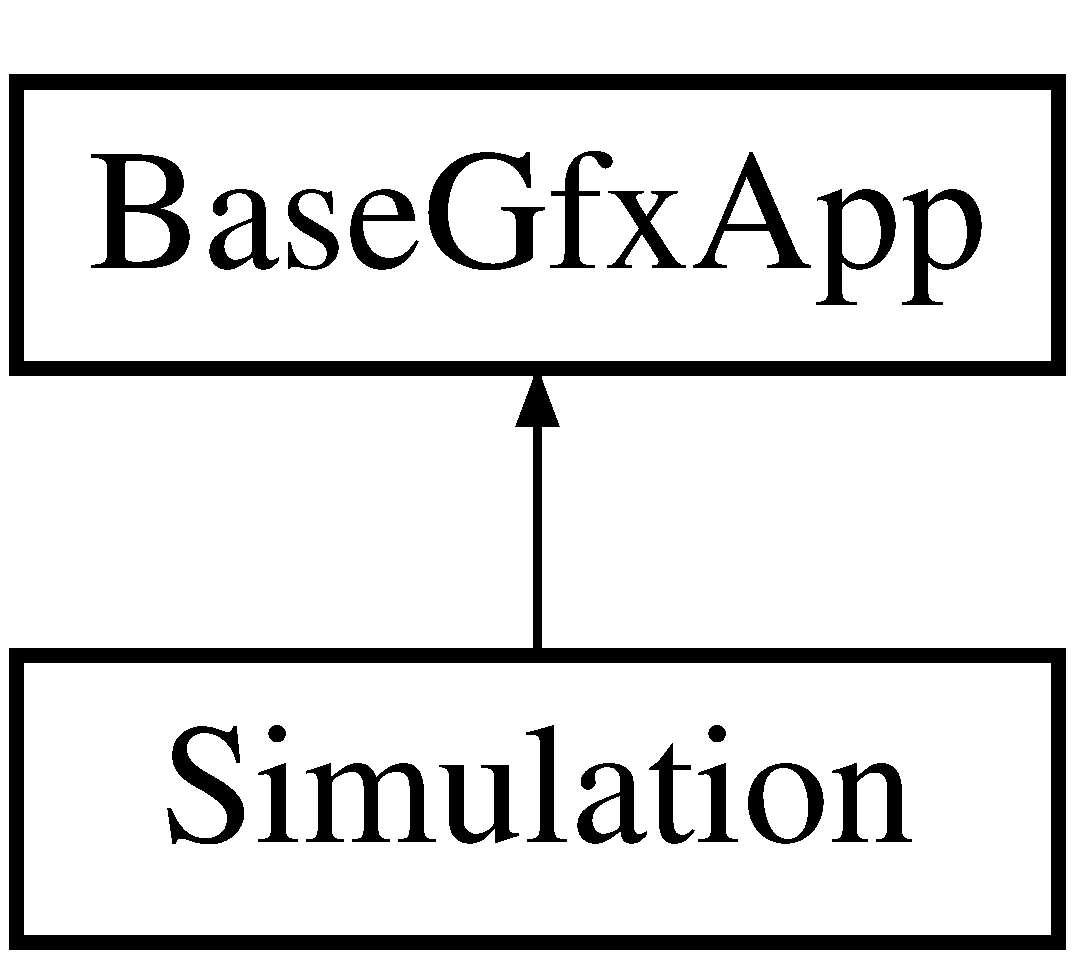
\includegraphics[height=2.000000cm]{classBaseGfxApp}
\end{center}
\end{figure}
\subsection*{Public Member Functions}
\begin{DoxyCompactItemize}
\item 
\hyperlink{classBaseGfxApp_a534a4b5293a35947fdae3805a103541d}{Base\-Gfx\-App} (int argc, char $\ast$argv\mbox{[}$\,$\mbox{]}, int \hyperlink{classBaseGfxApp_ace089a1a94fb6bb0bc17e1b7fa48e05d}{width}, int \hyperlink{classBaseGfxApp_aa253dbe16a20c40e0a1bf8ff942ceea3}{height}, int x, int y, int glut\-Flags, bool create\-G\-L\-U\-I\-Win, int glui\-Win\-X, int glui\-Win\-Y)
\item 
virtual \hyperlink{classBaseGfxApp_aceb6194bd818c0ffa980a6990fd03027}{$\sim$\-Base\-Gfx\-App} ()
\item 
void \hyperlink{classBaseGfxApp_a4b3b1a475b7f2babaf1b477c34b15fb1}{set\-Caption} (const std\-::string \&caption)
\item 
void \hyperlink{classBaseGfxApp_acda031916c00d56c2dc901e2653e3083}{run\-Main\-Loop} ()
\item 
virtual void \hyperlink{classBaseGfxApp_ac8de2d5a955582547af5619b771b4d6d}{display} ()
\item 
virtual void \hyperlink{classBaseGfxApp_a0956b82d7fa58b623c498aea7073dbba}{mouse\-Moved} (int x, int y)
\item 
virtual void \hyperlink{classBaseGfxApp_abb23f716dd6612b3a72938e41525d338}{mouse\-Dragged} (int x, int y)
\item 
virtual void \hyperlink{classBaseGfxApp_aaaccf5a5e923a9465441a5ee712424a8}{left\-Mouse\-Down} (int x, int y)
\item 
virtual void \hyperlink{classBaseGfxApp_a0a2961a932b02b2f9d7d0bb408f6fb51}{left\-Mouse\-Up} (int x, int y)
\item 
virtual void \hyperlink{classBaseGfxApp_afa87e6a71220945e41f0424e540125d9}{right\-Mouse\-Down} (int x, int y)
\item 
virtual void \hyperlink{classBaseGfxApp_a812643d563522a993457dd565c33f8f6}{right\-Mouse\-Up} (int x, int y)
\item 
virtual void \hyperlink{classBaseGfxApp_a2c98cae9bb5ad1fb1832a6d4812670f8}{middle\-Mouse\-Down} (int x, int y)
\item 
virtual void \hyperlink{classBaseGfxApp_a00fc05e8d9629b72302b5adf014bdb0c}{middle\-Mouse\-Up} (int x, int y)
\item 
virtual void \hyperlink{classBaseGfxApp_a6d91e0cb7a3d48cad33956efe7eb36ca}{keyboard} (unsigned char c, int x, int y)
\item 
virtual void \hyperlink{classBaseGfxApp_a345566e62c9e4ec3705ec4d1c4c75f1f}{keyboard\-Special} (int key, int x, int y)
\item 
virtual void \hyperlink{classBaseGfxApp_acc4a40ce11edd6b6660a19cb4802a2bf}{keyboard\-Up} (unsigned char c, int x, int y)
\item 
virtual void \hyperlink{classBaseGfxApp_afd14b435ff93b1e7f461cb8bd1a6fd59}{keyboard\-Special\-Up} (int key, int x, int y)
\item 
virtual void \hyperlink{classBaseGfxApp_a5d8d5d778a8aecd7f5f8e9c87f4c3d20}{reshape} (int \hyperlink{classBaseGfxApp_ace089a1a94fb6bb0bc17e1b7fa48e05d}{width}, int \hyperlink{classBaseGfxApp_aa253dbe16a20c40e0a1bf8ff942ceea3}{height})
\item 
virtual void \hyperlink{classBaseGfxApp_a2978a7c358794c67df73b66776b2cef3}{glui\-Control} (int control\-I\-D)
\item 
int \hyperlink{classBaseGfxApp_ace089a1a94fb6bb0bc17e1b7fa48e05d}{width} () const 
\item 
int \hyperlink{classBaseGfxApp_aa253dbe16a20c40e0a1bf8ff942ceea3}{height} () const 
\item 
int \hyperlink{classBaseGfxApp_ae9779f948eff6f45beec08091e98a803}{handle} ()
\item 
G\-L\-U\-I $\ast$ \hyperlink{classBaseGfxApp_ac721a0fedce80308c5c0e5695016e95d}{glui} ()
\end{DoxyCompactItemize}
\subsection*{Static Protected Member Functions}
\begin{DoxyCompactItemize}
\item 
static void \hyperlink{classBaseGfxApp_a5fe6a77d37044cbe28647ed3391bbb7a}{s\-\_\-reshape} (int \hyperlink{classBaseGfxApp_ace089a1a94fb6bb0bc17e1b7fa48e05d}{width}, int \hyperlink{classBaseGfxApp_aa253dbe16a20c40e0a1bf8ff942ceea3}{height})
\item 
static void \hyperlink{classBaseGfxApp_a52edb2569227319feb68779844e7d857}{s\-\_\-keyboard} (unsigned char c, int x, int y)
\item 
static void \hyperlink{classBaseGfxApp_a1e8d90a4faab60300ddf2a4ea9b83115}{s\-\_\-keyboardspecial} (int key, int x, int y)
\item 
static void \hyperlink{classBaseGfxApp_aa1ca205af9d6cee33949f2e6adf4c923}{s\-\_\-keyboardup} (unsigned char c, int x, int y)
\item 
static void \hyperlink{classBaseGfxApp_a0e4dfe006f3cc9126c1cc8ad32784f75}{s\-\_\-keyboardspecialup} (int key, int x, int y)
\item 
static void \hyperlink{classBaseGfxApp_a5e640f2394f7e038d0dd2b469d5c2e24}{s\-\_\-mousemotion} (int x, int y)
\item 
static void \hyperlink{classBaseGfxApp_a22dd953bfb75add9fd0f8f2f8be535c5}{s\-\_\-mousebtn} (int b, int s, int x, int y)
\item 
static void \hyperlink{classBaseGfxApp_a58415c6151a2a80e1fe2eaa9919a4dab}{s\-\_\-draw} ()
\item 
static void \hyperlink{classBaseGfxApp_ad4a963321f1147d68369225ab0c7f32f}{s\-\_\-gluicallback} (int control\-I\-D)
\end{DoxyCompactItemize}
\subsection*{Protected Attributes}
\begin{DoxyCompactItemize}
\item 
int \hyperlink{classBaseGfxApp_ad8697d6fdd10e6f336c3a662016b4fa7}{m\-\_\-glut\-Window\-Handle}
\item 
G\-L\-U\-I $\ast$ \hyperlink{classBaseGfxApp_a6eb1673b80283727221da2242211af1d}{m\-\_\-glui}
\item 
bool \hyperlink{classBaseGfxApp_a2e70a389224f8affe7c137f7e20dc8c1}{m\-\_\-drag}
\item 
int \hyperlink{classBaseGfxApp_a7e5ef1c8f25fe081b4a1fd4ce6a96e07}{m\-\_\-width}
\item 
int \hyperlink{classBaseGfxApp_ac078e4fc20b5c2fe0c744966b850b412}{m\-\_\-height}
\end{DoxyCompactItemize}
\subsection*{Static Protected Attributes}
\begin{DoxyCompactItemize}
\item 
static \hyperlink{classBaseGfxApp}{Base\-Gfx\-App} $\ast$ \hyperlink{classBaseGfxApp_a65ba89b98af31e2649a0546631931000}{s\-\_\-current\-App} = N\-U\-L\-L
\item 
static bool \hyperlink{classBaseGfxApp_afa4690383ea27713016ef75b9fb1e42f}{s\-\_\-glut\-Initialized} = false
\end{DoxyCompactItemize}


\subsection{Constructor \& Destructor Documentation}
\hypertarget{classBaseGfxApp_a534a4b5293a35947fdae3805a103541d}{\index{Base\-Gfx\-App@{Base\-Gfx\-App}!Base\-Gfx\-App@{Base\-Gfx\-App}}
\index{Base\-Gfx\-App@{Base\-Gfx\-App}!BaseGfxApp@{Base\-Gfx\-App}}
\subsubsection[{Base\-Gfx\-App}]{\setlength{\rightskip}{0pt plus 5cm}Base\-Gfx\-App\-::\-Base\-Gfx\-App (
\begin{DoxyParamCaption}
\item[{int}]{argc, }
\item[{char $\ast$}]{argv\mbox{[}$\,$\mbox{]}, }
\item[{int}]{width, }
\item[{int}]{height, }
\item[{int}]{x, }
\item[{int}]{y, }
\item[{int}]{glut\-Flags, }
\item[{bool}]{create\-G\-L\-U\-I\-Win, }
\item[{int}]{glui\-Win\-X, }
\item[{int}]{glui\-Win\-Y}
\end{DoxyParamCaption}
)}}\label{classBaseGfxApp_a534a4b5293a35947fdae3805a103541d}
\hypertarget{classBaseGfxApp_aceb6194bd818c0ffa980a6990fd03027}{\index{Base\-Gfx\-App@{Base\-Gfx\-App}!$\sim$\-Base\-Gfx\-App@{$\sim$\-Base\-Gfx\-App}}
\index{$\sim$\-Base\-Gfx\-App@{$\sim$\-Base\-Gfx\-App}!BaseGfxApp@{Base\-Gfx\-App}}
\subsubsection[{$\sim$\-Base\-Gfx\-App}]{\setlength{\rightskip}{0pt plus 5cm}Base\-Gfx\-App\-::$\sim$\-Base\-Gfx\-App (
\begin{DoxyParamCaption}
{}
\end{DoxyParamCaption}
)\hspace{0.3cm}{\ttfamily [virtual]}}}\label{classBaseGfxApp_aceb6194bd818c0ffa980a6990fd03027}


\subsection{Member Function Documentation}
\hypertarget{classBaseGfxApp_ac8de2d5a955582547af5619b771b4d6d}{\index{Base\-Gfx\-App@{Base\-Gfx\-App}!display@{display}}
\index{display@{display}!BaseGfxApp@{Base\-Gfx\-App}}
\subsubsection[{display}]{\setlength{\rightskip}{0pt plus 5cm}virtual void Base\-Gfx\-App\-::display (
\begin{DoxyParamCaption}
{}
\end{DoxyParamCaption}
)\hspace{0.3cm}{\ttfamily [inline]}, {\ttfamily [virtual]}}}\label{classBaseGfxApp_ac8de2d5a955582547af5619b771b4d6d}


Reimplemented in \hyperlink{classSimulation_a449dcb7d97dfba99efe770de2f399c31}{Simulation}.

\hypertarget{classBaseGfxApp_ac721a0fedce80308c5c0e5695016e95d}{\index{Base\-Gfx\-App@{Base\-Gfx\-App}!glui@{glui}}
\index{glui@{glui}!BaseGfxApp@{Base\-Gfx\-App}}
\subsubsection[{glui}]{\setlength{\rightskip}{0pt plus 5cm}G\-L\-U\-I$\ast$ Base\-Gfx\-App\-::glui (
\begin{DoxyParamCaption}
{}
\end{DoxyParamCaption}
)\hspace{0.3cm}{\ttfamily [inline]}}}\label{classBaseGfxApp_ac721a0fedce80308c5c0e5695016e95d}
\hypertarget{classBaseGfxApp_a2978a7c358794c67df73b66776b2cef3}{\index{Base\-Gfx\-App@{Base\-Gfx\-App}!glui\-Control@{glui\-Control}}
\index{glui\-Control@{glui\-Control}!BaseGfxApp@{Base\-Gfx\-App}}
\subsubsection[{glui\-Control}]{\setlength{\rightskip}{0pt plus 5cm}virtual void Base\-Gfx\-App\-::glui\-Control (
\begin{DoxyParamCaption}
\item[{int}]{control\-I\-D}
\end{DoxyParamCaption}
)\hspace{0.3cm}{\ttfamily [inline]}, {\ttfamily [virtual]}}}\label{classBaseGfxApp_a2978a7c358794c67df73b66776b2cef3}


Reimplemented in \hyperlink{classSimulation_a1607cd18e552ab9f4a6f57d362f7121a}{Simulation}.

\hypertarget{classBaseGfxApp_ae9779f948eff6f45beec08091e98a803}{\index{Base\-Gfx\-App@{Base\-Gfx\-App}!handle@{handle}}
\index{handle@{handle}!BaseGfxApp@{Base\-Gfx\-App}}
\subsubsection[{handle}]{\setlength{\rightskip}{0pt plus 5cm}int Base\-Gfx\-App\-::handle (
\begin{DoxyParamCaption}
{}
\end{DoxyParamCaption}
)\hspace{0.3cm}{\ttfamily [inline]}}}\label{classBaseGfxApp_ae9779f948eff6f45beec08091e98a803}
\hypertarget{classBaseGfxApp_aa253dbe16a20c40e0a1bf8ff942ceea3}{\index{Base\-Gfx\-App@{Base\-Gfx\-App}!height@{height}}
\index{height@{height}!BaseGfxApp@{Base\-Gfx\-App}}
\subsubsection[{height}]{\setlength{\rightskip}{0pt plus 5cm}int Base\-Gfx\-App\-::height (
\begin{DoxyParamCaption}
{}
\end{DoxyParamCaption}
) const}}\label{classBaseGfxApp_aa253dbe16a20c40e0a1bf8ff942ceea3}
\hypertarget{classBaseGfxApp_a6d91e0cb7a3d48cad33956efe7eb36ca}{\index{Base\-Gfx\-App@{Base\-Gfx\-App}!keyboard@{keyboard}}
\index{keyboard@{keyboard}!BaseGfxApp@{Base\-Gfx\-App}}
\subsubsection[{keyboard}]{\setlength{\rightskip}{0pt plus 5cm}virtual void Base\-Gfx\-App\-::keyboard (
\begin{DoxyParamCaption}
\item[{unsigned char}]{c, }
\item[{int}]{x, }
\item[{int}]{y}
\end{DoxyParamCaption}
)\hspace{0.3cm}{\ttfamily [inline]}, {\ttfamily [virtual]}}}\label{classBaseGfxApp_a6d91e0cb7a3d48cad33956efe7eb36ca}
\hypertarget{classBaseGfxApp_a345566e62c9e4ec3705ec4d1c4c75f1f}{\index{Base\-Gfx\-App@{Base\-Gfx\-App}!keyboard\-Special@{keyboard\-Special}}
\index{keyboard\-Special@{keyboard\-Special}!BaseGfxApp@{Base\-Gfx\-App}}
\subsubsection[{keyboard\-Special}]{\setlength{\rightskip}{0pt plus 5cm}virtual void Base\-Gfx\-App\-::keyboard\-Special (
\begin{DoxyParamCaption}
\item[{int}]{key, }
\item[{int}]{x, }
\item[{int}]{y}
\end{DoxyParamCaption}
)\hspace{0.3cm}{\ttfamily [inline]}, {\ttfamily [virtual]}}}\label{classBaseGfxApp_a345566e62c9e4ec3705ec4d1c4c75f1f}
\hypertarget{classBaseGfxApp_afd14b435ff93b1e7f461cb8bd1a6fd59}{\index{Base\-Gfx\-App@{Base\-Gfx\-App}!keyboard\-Special\-Up@{keyboard\-Special\-Up}}
\index{keyboard\-Special\-Up@{keyboard\-Special\-Up}!BaseGfxApp@{Base\-Gfx\-App}}
\subsubsection[{keyboard\-Special\-Up}]{\setlength{\rightskip}{0pt plus 5cm}virtual void Base\-Gfx\-App\-::keyboard\-Special\-Up (
\begin{DoxyParamCaption}
\item[{int}]{key, }
\item[{int}]{x, }
\item[{int}]{y}
\end{DoxyParamCaption}
)\hspace{0.3cm}{\ttfamily [inline]}, {\ttfamily [virtual]}}}\label{classBaseGfxApp_afd14b435ff93b1e7f461cb8bd1a6fd59}
\hypertarget{classBaseGfxApp_acc4a40ce11edd6b6660a19cb4802a2bf}{\index{Base\-Gfx\-App@{Base\-Gfx\-App}!keyboard\-Up@{keyboard\-Up}}
\index{keyboard\-Up@{keyboard\-Up}!BaseGfxApp@{Base\-Gfx\-App}}
\subsubsection[{keyboard\-Up}]{\setlength{\rightskip}{0pt plus 5cm}virtual void Base\-Gfx\-App\-::keyboard\-Up (
\begin{DoxyParamCaption}
\item[{unsigned char}]{c, }
\item[{int}]{x, }
\item[{int}]{y}
\end{DoxyParamCaption}
)\hspace{0.3cm}{\ttfamily [inline]}, {\ttfamily [virtual]}}}\label{classBaseGfxApp_acc4a40ce11edd6b6660a19cb4802a2bf}
\hypertarget{classBaseGfxApp_aaaccf5a5e923a9465441a5ee712424a8}{\index{Base\-Gfx\-App@{Base\-Gfx\-App}!left\-Mouse\-Down@{left\-Mouse\-Down}}
\index{left\-Mouse\-Down@{left\-Mouse\-Down}!BaseGfxApp@{Base\-Gfx\-App}}
\subsubsection[{left\-Mouse\-Down}]{\setlength{\rightskip}{0pt plus 5cm}virtual void Base\-Gfx\-App\-::left\-Mouse\-Down (
\begin{DoxyParamCaption}
\item[{int}]{x, }
\item[{int}]{y}
\end{DoxyParamCaption}
)\hspace{0.3cm}{\ttfamily [inline]}, {\ttfamily [virtual]}}}\label{classBaseGfxApp_aaaccf5a5e923a9465441a5ee712424a8}


Reimplemented in \hyperlink{classSimulation_a786d1ba31d29937f0ac6f3ea88f8a607}{Simulation}.

\hypertarget{classBaseGfxApp_a0a2961a932b02b2f9d7d0bb408f6fb51}{\index{Base\-Gfx\-App@{Base\-Gfx\-App}!left\-Mouse\-Up@{left\-Mouse\-Up}}
\index{left\-Mouse\-Up@{left\-Mouse\-Up}!BaseGfxApp@{Base\-Gfx\-App}}
\subsubsection[{left\-Mouse\-Up}]{\setlength{\rightskip}{0pt plus 5cm}virtual void Base\-Gfx\-App\-::left\-Mouse\-Up (
\begin{DoxyParamCaption}
\item[{int}]{x, }
\item[{int}]{y}
\end{DoxyParamCaption}
)\hspace{0.3cm}{\ttfamily [inline]}, {\ttfamily [virtual]}}}\label{classBaseGfxApp_a0a2961a932b02b2f9d7d0bb408f6fb51}


Reimplemented in \hyperlink{classSimulation_a62ef254d85017074cd521a5787b5a234}{Simulation}.

\hypertarget{classBaseGfxApp_a2c98cae9bb5ad1fb1832a6d4812670f8}{\index{Base\-Gfx\-App@{Base\-Gfx\-App}!middle\-Mouse\-Down@{middle\-Mouse\-Down}}
\index{middle\-Mouse\-Down@{middle\-Mouse\-Down}!BaseGfxApp@{Base\-Gfx\-App}}
\subsubsection[{middle\-Mouse\-Down}]{\setlength{\rightskip}{0pt plus 5cm}virtual void Base\-Gfx\-App\-::middle\-Mouse\-Down (
\begin{DoxyParamCaption}
\item[{int}]{x, }
\item[{int}]{y}
\end{DoxyParamCaption}
)\hspace{0.3cm}{\ttfamily [inline]}, {\ttfamily [virtual]}}}\label{classBaseGfxApp_a2c98cae9bb5ad1fb1832a6d4812670f8}
\hypertarget{classBaseGfxApp_a00fc05e8d9629b72302b5adf014bdb0c}{\index{Base\-Gfx\-App@{Base\-Gfx\-App}!middle\-Mouse\-Up@{middle\-Mouse\-Up}}
\index{middle\-Mouse\-Up@{middle\-Mouse\-Up}!BaseGfxApp@{Base\-Gfx\-App}}
\subsubsection[{middle\-Mouse\-Up}]{\setlength{\rightskip}{0pt plus 5cm}virtual void Base\-Gfx\-App\-::middle\-Mouse\-Up (
\begin{DoxyParamCaption}
\item[{int}]{x, }
\item[{int}]{y}
\end{DoxyParamCaption}
)\hspace{0.3cm}{\ttfamily [inline]}, {\ttfamily [virtual]}}}\label{classBaseGfxApp_a00fc05e8d9629b72302b5adf014bdb0c}
\hypertarget{classBaseGfxApp_abb23f716dd6612b3a72938e41525d338}{\index{Base\-Gfx\-App@{Base\-Gfx\-App}!mouse\-Dragged@{mouse\-Dragged}}
\index{mouse\-Dragged@{mouse\-Dragged}!BaseGfxApp@{Base\-Gfx\-App}}
\subsubsection[{mouse\-Dragged}]{\setlength{\rightskip}{0pt plus 5cm}virtual void Base\-Gfx\-App\-::mouse\-Dragged (
\begin{DoxyParamCaption}
\item[{int}]{x, }
\item[{int}]{y}
\end{DoxyParamCaption}
)\hspace{0.3cm}{\ttfamily [inline]}, {\ttfamily [virtual]}}}\label{classBaseGfxApp_abb23f716dd6612b3a72938e41525d338}
\hypertarget{classBaseGfxApp_a0956b82d7fa58b623c498aea7073dbba}{\index{Base\-Gfx\-App@{Base\-Gfx\-App}!mouse\-Moved@{mouse\-Moved}}
\index{mouse\-Moved@{mouse\-Moved}!BaseGfxApp@{Base\-Gfx\-App}}
\subsubsection[{mouse\-Moved}]{\setlength{\rightskip}{0pt plus 5cm}virtual void Base\-Gfx\-App\-::mouse\-Moved (
\begin{DoxyParamCaption}
\item[{int}]{x, }
\item[{int}]{y}
\end{DoxyParamCaption}
)\hspace{0.3cm}{\ttfamily [inline]}, {\ttfamily [virtual]}}}\label{classBaseGfxApp_a0956b82d7fa58b623c498aea7073dbba}
\hypertarget{classBaseGfxApp_a5d8d5d778a8aecd7f5f8e9c87f4c3d20}{\index{Base\-Gfx\-App@{Base\-Gfx\-App}!reshape@{reshape}}
\index{reshape@{reshape}!BaseGfxApp@{Base\-Gfx\-App}}
\subsubsection[{reshape}]{\setlength{\rightskip}{0pt plus 5cm}void Base\-Gfx\-App\-::reshape (
\begin{DoxyParamCaption}
\item[{int}]{width, }
\item[{int}]{height}
\end{DoxyParamCaption}
)\hspace{0.3cm}{\ttfamily [virtual]}}}\label{classBaseGfxApp_a5d8d5d778a8aecd7f5f8e9c87f4c3d20}
\hypertarget{classBaseGfxApp_afa87e6a71220945e41f0424e540125d9}{\index{Base\-Gfx\-App@{Base\-Gfx\-App}!right\-Mouse\-Down@{right\-Mouse\-Down}}
\index{right\-Mouse\-Down@{right\-Mouse\-Down}!BaseGfxApp@{Base\-Gfx\-App}}
\subsubsection[{right\-Mouse\-Down}]{\setlength{\rightskip}{0pt plus 5cm}virtual void Base\-Gfx\-App\-::right\-Mouse\-Down (
\begin{DoxyParamCaption}
\item[{int}]{x, }
\item[{int}]{y}
\end{DoxyParamCaption}
)\hspace{0.3cm}{\ttfamily [inline]}, {\ttfamily [virtual]}}}\label{classBaseGfxApp_afa87e6a71220945e41f0424e540125d9}
\hypertarget{classBaseGfxApp_a812643d563522a993457dd565c33f8f6}{\index{Base\-Gfx\-App@{Base\-Gfx\-App}!right\-Mouse\-Up@{right\-Mouse\-Up}}
\index{right\-Mouse\-Up@{right\-Mouse\-Up}!BaseGfxApp@{Base\-Gfx\-App}}
\subsubsection[{right\-Mouse\-Up}]{\setlength{\rightskip}{0pt plus 5cm}virtual void Base\-Gfx\-App\-::right\-Mouse\-Up (
\begin{DoxyParamCaption}
\item[{int}]{x, }
\item[{int}]{y}
\end{DoxyParamCaption}
)\hspace{0.3cm}{\ttfamily [inline]}, {\ttfamily [virtual]}}}\label{classBaseGfxApp_a812643d563522a993457dd565c33f8f6}
\hypertarget{classBaseGfxApp_acda031916c00d56c2dc901e2653e3083}{\index{Base\-Gfx\-App@{Base\-Gfx\-App}!run\-Main\-Loop@{run\-Main\-Loop}}
\index{run\-Main\-Loop@{run\-Main\-Loop}!BaseGfxApp@{Base\-Gfx\-App}}
\subsubsection[{run\-Main\-Loop}]{\setlength{\rightskip}{0pt plus 5cm}void Base\-Gfx\-App\-::run\-Main\-Loop (
\begin{DoxyParamCaption}
{}
\end{DoxyParamCaption}
)}}\label{classBaseGfxApp_acda031916c00d56c2dc901e2653e3083}
\hypertarget{classBaseGfxApp_a58415c6151a2a80e1fe2eaa9919a4dab}{\index{Base\-Gfx\-App@{Base\-Gfx\-App}!s\-\_\-draw@{s\-\_\-draw}}
\index{s\-\_\-draw@{s\-\_\-draw}!BaseGfxApp@{Base\-Gfx\-App}}
\subsubsection[{s\-\_\-draw}]{\setlength{\rightskip}{0pt plus 5cm}void Base\-Gfx\-App\-::s\-\_\-draw (
\begin{DoxyParamCaption}
{}
\end{DoxyParamCaption}
)\hspace{0.3cm}{\ttfamily [static]}, {\ttfamily [protected]}}}\label{classBaseGfxApp_a58415c6151a2a80e1fe2eaa9919a4dab}
\hypertarget{classBaseGfxApp_ad4a963321f1147d68369225ab0c7f32f}{\index{Base\-Gfx\-App@{Base\-Gfx\-App}!s\-\_\-gluicallback@{s\-\_\-gluicallback}}
\index{s\-\_\-gluicallback@{s\-\_\-gluicallback}!BaseGfxApp@{Base\-Gfx\-App}}
\subsubsection[{s\-\_\-gluicallback}]{\setlength{\rightskip}{0pt plus 5cm}void Base\-Gfx\-App\-::s\-\_\-gluicallback (
\begin{DoxyParamCaption}
\item[{int}]{control\-I\-D}
\end{DoxyParamCaption}
)\hspace{0.3cm}{\ttfamily [static]}, {\ttfamily [protected]}}}\label{classBaseGfxApp_ad4a963321f1147d68369225ab0c7f32f}
\hypertarget{classBaseGfxApp_a52edb2569227319feb68779844e7d857}{\index{Base\-Gfx\-App@{Base\-Gfx\-App}!s\-\_\-keyboard@{s\-\_\-keyboard}}
\index{s\-\_\-keyboard@{s\-\_\-keyboard}!BaseGfxApp@{Base\-Gfx\-App}}
\subsubsection[{s\-\_\-keyboard}]{\setlength{\rightskip}{0pt plus 5cm}void Base\-Gfx\-App\-::s\-\_\-keyboard (
\begin{DoxyParamCaption}
\item[{unsigned char}]{c, }
\item[{int}]{x, }
\item[{int}]{y}
\end{DoxyParamCaption}
)\hspace{0.3cm}{\ttfamily [static]}, {\ttfamily [protected]}}}\label{classBaseGfxApp_a52edb2569227319feb68779844e7d857}
\hypertarget{classBaseGfxApp_a1e8d90a4faab60300ddf2a4ea9b83115}{\index{Base\-Gfx\-App@{Base\-Gfx\-App}!s\-\_\-keyboardspecial@{s\-\_\-keyboardspecial}}
\index{s\-\_\-keyboardspecial@{s\-\_\-keyboardspecial}!BaseGfxApp@{Base\-Gfx\-App}}
\subsubsection[{s\-\_\-keyboardspecial}]{\setlength{\rightskip}{0pt plus 5cm}void Base\-Gfx\-App\-::s\-\_\-keyboardspecial (
\begin{DoxyParamCaption}
\item[{int}]{key, }
\item[{int}]{x, }
\item[{int}]{y}
\end{DoxyParamCaption}
)\hspace{0.3cm}{\ttfamily [static]}, {\ttfamily [protected]}}}\label{classBaseGfxApp_a1e8d90a4faab60300ddf2a4ea9b83115}
\hypertarget{classBaseGfxApp_a0e4dfe006f3cc9126c1cc8ad32784f75}{\index{Base\-Gfx\-App@{Base\-Gfx\-App}!s\-\_\-keyboardspecialup@{s\-\_\-keyboardspecialup}}
\index{s\-\_\-keyboardspecialup@{s\-\_\-keyboardspecialup}!BaseGfxApp@{Base\-Gfx\-App}}
\subsubsection[{s\-\_\-keyboardspecialup}]{\setlength{\rightskip}{0pt plus 5cm}void Base\-Gfx\-App\-::s\-\_\-keyboardspecialup (
\begin{DoxyParamCaption}
\item[{int}]{key, }
\item[{int}]{x, }
\item[{int}]{y}
\end{DoxyParamCaption}
)\hspace{0.3cm}{\ttfamily [static]}, {\ttfamily [protected]}}}\label{classBaseGfxApp_a0e4dfe006f3cc9126c1cc8ad32784f75}
\hypertarget{classBaseGfxApp_aa1ca205af9d6cee33949f2e6adf4c923}{\index{Base\-Gfx\-App@{Base\-Gfx\-App}!s\-\_\-keyboardup@{s\-\_\-keyboardup}}
\index{s\-\_\-keyboardup@{s\-\_\-keyboardup}!BaseGfxApp@{Base\-Gfx\-App}}
\subsubsection[{s\-\_\-keyboardup}]{\setlength{\rightskip}{0pt plus 5cm}void Base\-Gfx\-App\-::s\-\_\-keyboardup (
\begin{DoxyParamCaption}
\item[{unsigned char}]{c, }
\item[{int}]{x, }
\item[{int}]{y}
\end{DoxyParamCaption}
)\hspace{0.3cm}{\ttfamily [static]}, {\ttfamily [protected]}}}\label{classBaseGfxApp_aa1ca205af9d6cee33949f2e6adf4c923}
\hypertarget{classBaseGfxApp_a22dd953bfb75add9fd0f8f2f8be535c5}{\index{Base\-Gfx\-App@{Base\-Gfx\-App}!s\-\_\-mousebtn@{s\-\_\-mousebtn}}
\index{s\-\_\-mousebtn@{s\-\_\-mousebtn}!BaseGfxApp@{Base\-Gfx\-App}}
\subsubsection[{s\-\_\-mousebtn}]{\setlength{\rightskip}{0pt plus 5cm}void Base\-Gfx\-App\-::s\-\_\-mousebtn (
\begin{DoxyParamCaption}
\item[{int}]{b, }
\item[{int}]{s, }
\item[{int}]{x, }
\item[{int}]{y}
\end{DoxyParamCaption}
)\hspace{0.3cm}{\ttfamily [static]}, {\ttfamily [protected]}}}\label{classBaseGfxApp_a22dd953bfb75add9fd0f8f2f8be535c5}
\hypertarget{classBaseGfxApp_a5e640f2394f7e038d0dd2b469d5c2e24}{\index{Base\-Gfx\-App@{Base\-Gfx\-App}!s\-\_\-mousemotion@{s\-\_\-mousemotion}}
\index{s\-\_\-mousemotion@{s\-\_\-mousemotion}!BaseGfxApp@{Base\-Gfx\-App}}
\subsubsection[{s\-\_\-mousemotion}]{\setlength{\rightskip}{0pt plus 5cm}void Base\-Gfx\-App\-::s\-\_\-mousemotion (
\begin{DoxyParamCaption}
\item[{int}]{x, }
\item[{int}]{y}
\end{DoxyParamCaption}
)\hspace{0.3cm}{\ttfamily [static]}, {\ttfamily [protected]}}}\label{classBaseGfxApp_a5e640f2394f7e038d0dd2b469d5c2e24}
\hypertarget{classBaseGfxApp_a5fe6a77d37044cbe28647ed3391bbb7a}{\index{Base\-Gfx\-App@{Base\-Gfx\-App}!s\-\_\-reshape@{s\-\_\-reshape}}
\index{s\-\_\-reshape@{s\-\_\-reshape}!BaseGfxApp@{Base\-Gfx\-App}}
\subsubsection[{s\-\_\-reshape}]{\setlength{\rightskip}{0pt plus 5cm}void Base\-Gfx\-App\-::s\-\_\-reshape (
\begin{DoxyParamCaption}
\item[{int}]{width, }
\item[{int}]{height}
\end{DoxyParamCaption}
)\hspace{0.3cm}{\ttfamily [static]}, {\ttfamily [protected]}}}\label{classBaseGfxApp_a5fe6a77d37044cbe28647ed3391bbb7a}
\hypertarget{classBaseGfxApp_a4b3b1a475b7f2babaf1b477c34b15fb1}{\index{Base\-Gfx\-App@{Base\-Gfx\-App}!set\-Caption@{set\-Caption}}
\index{set\-Caption@{set\-Caption}!BaseGfxApp@{Base\-Gfx\-App}}
\subsubsection[{set\-Caption}]{\setlength{\rightskip}{0pt plus 5cm}void Base\-Gfx\-App\-::set\-Caption (
\begin{DoxyParamCaption}
\item[{const std\-::string \&}]{caption}
\end{DoxyParamCaption}
)}}\label{classBaseGfxApp_a4b3b1a475b7f2babaf1b477c34b15fb1}
\hypertarget{classBaseGfxApp_ace089a1a94fb6bb0bc17e1b7fa48e05d}{\index{Base\-Gfx\-App@{Base\-Gfx\-App}!width@{width}}
\index{width@{width}!BaseGfxApp@{Base\-Gfx\-App}}
\subsubsection[{width}]{\setlength{\rightskip}{0pt plus 5cm}int Base\-Gfx\-App\-::width (
\begin{DoxyParamCaption}
{}
\end{DoxyParamCaption}
) const}}\label{classBaseGfxApp_ace089a1a94fb6bb0bc17e1b7fa48e05d}


\subsection{Member Data Documentation}
\hypertarget{classBaseGfxApp_a2e70a389224f8affe7c137f7e20dc8c1}{\index{Base\-Gfx\-App@{Base\-Gfx\-App}!m\-\_\-drag@{m\-\_\-drag}}
\index{m\-\_\-drag@{m\-\_\-drag}!BaseGfxApp@{Base\-Gfx\-App}}
\subsubsection[{m\-\_\-drag}]{\setlength{\rightskip}{0pt plus 5cm}bool Base\-Gfx\-App\-::m\-\_\-drag\hspace{0.3cm}{\ttfamily [protected]}}}\label{classBaseGfxApp_a2e70a389224f8affe7c137f7e20dc8c1}
\hypertarget{classBaseGfxApp_a6eb1673b80283727221da2242211af1d}{\index{Base\-Gfx\-App@{Base\-Gfx\-App}!m\-\_\-glui@{m\-\_\-glui}}
\index{m\-\_\-glui@{m\-\_\-glui}!BaseGfxApp@{Base\-Gfx\-App}}
\subsubsection[{m\-\_\-glui}]{\setlength{\rightskip}{0pt plus 5cm}G\-L\-U\-I$\ast$ Base\-Gfx\-App\-::m\-\_\-glui\hspace{0.3cm}{\ttfamily [protected]}}}\label{classBaseGfxApp_a6eb1673b80283727221da2242211af1d}
\hypertarget{classBaseGfxApp_ad8697d6fdd10e6f336c3a662016b4fa7}{\index{Base\-Gfx\-App@{Base\-Gfx\-App}!m\-\_\-glut\-Window\-Handle@{m\-\_\-glut\-Window\-Handle}}
\index{m\-\_\-glut\-Window\-Handle@{m\-\_\-glut\-Window\-Handle}!BaseGfxApp@{Base\-Gfx\-App}}
\subsubsection[{m\-\_\-glut\-Window\-Handle}]{\setlength{\rightskip}{0pt plus 5cm}int Base\-Gfx\-App\-::m\-\_\-glut\-Window\-Handle\hspace{0.3cm}{\ttfamily [protected]}}}\label{classBaseGfxApp_ad8697d6fdd10e6f336c3a662016b4fa7}
Underlying glut window handle \hypertarget{classBaseGfxApp_ac078e4fc20b5c2fe0c744966b850b412}{\index{Base\-Gfx\-App@{Base\-Gfx\-App}!m\-\_\-height@{m\-\_\-height}}
\index{m\-\_\-height@{m\-\_\-height}!BaseGfxApp@{Base\-Gfx\-App}}
\subsubsection[{m\-\_\-height}]{\setlength{\rightskip}{0pt plus 5cm}int Base\-Gfx\-App\-::m\-\_\-height\hspace{0.3cm}{\ttfamily [protected]}}}\label{classBaseGfxApp_ac078e4fc20b5c2fe0c744966b850b412}
\hypertarget{classBaseGfxApp_a7e5ef1c8f25fe081b4a1fd4ce6a96e07}{\index{Base\-Gfx\-App@{Base\-Gfx\-App}!m\-\_\-width@{m\-\_\-width}}
\index{m\-\_\-width@{m\-\_\-width}!BaseGfxApp@{Base\-Gfx\-App}}
\subsubsection[{m\-\_\-width}]{\setlength{\rightskip}{0pt plus 5cm}int Base\-Gfx\-App\-::m\-\_\-width\hspace{0.3cm}{\ttfamily [protected]}}}\label{classBaseGfxApp_a7e5ef1c8f25fe081b4a1fd4ce6a96e07}
\hypertarget{classBaseGfxApp_a65ba89b98af31e2649a0546631931000}{\index{Base\-Gfx\-App@{Base\-Gfx\-App}!s\-\_\-current\-App@{s\-\_\-current\-App}}
\index{s\-\_\-current\-App@{s\-\_\-current\-App}!BaseGfxApp@{Base\-Gfx\-App}}
\subsubsection[{s\-\_\-current\-App}]{\setlength{\rightskip}{0pt plus 5cm}{\bf Base\-Gfx\-App} $\ast$ Base\-Gfx\-App\-::s\-\_\-current\-App = N\-U\-L\-L\hspace{0.3cm}{\ttfamily [static]}, {\ttfamily [protected]}}}\label{classBaseGfxApp_a65ba89b98af31e2649a0546631931000}
G\-L\-U\-T and G\-L\-U\-I event callbacks are sent to the current window/app. Right now, there is only one window anyway (not counting the G\-L\-U\-I U\-I window.. in the future could be extended to support more windows. In any case, some structure like this is always needed when using glut with C++, since the glut callbacks must be either global or static functions. \hypertarget{classBaseGfxApp_afa4690383ea27713016ef75b9fb1e42f}{\index{Base\-Gfx\-App@{Base\-Gfx\-App}!s\-\_\-glut\-Initialized@{s\-\_\-glut\-Initialized}}
\index{s\-\_\-glut\-Initialized@{s\-\_\-glut\-Initialized}!BaseGfxApp@{Base\-Gfx\-App}}
\subsubsection[{s\-\_\-glut\-Initialized}]{\setlength{\rightskip}{0pt plus 5cm}bool Base\-Gfx\-App\-::s\-\_\-glut\-Initialized = false\hspace{0.3cm}{\ttfamily [static]}, {\ttfamily [protected]}}}\label{classBaseGfxApp_afa4690383ea27713016ef75b9fb1e42f}
Has glut\-Init been called? (only allowed once per program) 

The documentation for this class was generated from the following files\-:\begin{DoxyCompactItemize}
\item 
\hyperlink{BaseGfxApp_8h}{Base\-Gfx\-App.\-h}\item 
\hyperlink{BaseGfxApp_8cpp}{Base\-Gfx\-App.\-cpp}\end{DoxyCompactItemize}

\hypertarget{classEnvironmentClass}{\section{Environment\-Class Class Reference}
\label{classEnvironmentClass}\index{Environment\-Class@{Environment\-Class}}
}


{\ttfamily \#include $<$Environment\-Class.\-h$>$}

\subsection*{Public Member Functions}
\begin{DoxyCompactItemize}
\item 
\hyperlink{classEnvironmentClass_aa69ad01551a79f7326f005709061ff31}{Environment\-Class} ()
\begin{DoxyCompactList}\small\item\em The default constructor. \end{DoxyCompactList}\item 
\hyperlink{classEnvironmentClass_a48da88b6cf7894159825b9c869b2af9f}{Environment\-Class} (int area, int width, int height, std\-::vector$<$ \hyperlink{classObject}{Object} $>$ $\ast$objs)
\begin{DoxyCompactList}\small\item\em A Constructor. \end{DoxyCompactList}\item 
void \hyperlink{classEnvironmentClass_afd86169390f7e3aadfb7b6438d220655}{update} (double elasped\-Time)
\begin{DoxyCompactList}\small\item\em Update the orientation and positions of each object. \end{DoxyCompactList}\item 
int \hyperlink{classEnvironmentClass_a77e1650c9944e5831760b4f9a9482580}{get\-Count} ()
\begin{DoxyCompactList}\small\item\em This function returns the number of objects in the environment. \end{DoxyCompactList}\item 
void \hyperlink{classEnvironmentClass_ac4de88a208dfe69c635eb1aa1954fc60}{register\-Object} (\hyperlink{classObject}{Object} obj)
\begin{DoxyCompactList}\small\item\em Objects register with the environment, which adds them to the environment data structure(s). \end{DoxyCompactList}\item 
int \hyperlink{classEnvironmentClass_a401ac57c648ba38b9ff5e29699ae0e2a}{touch\-Sensor\-Reading} (\hyperlink{classObject}{Object} obj)
\begin{DoxyCompactList}\small\item\em This function returns the information about distance and angles between each pair of robot and target. The infomation is returned in form of distance-\/direction vector. \end{DoxyCompactList}\item 
\hyperlink{structNavigate}{Navigate} \hyperlink{classEnvironmentClass_a4535aab681606c4b67e790ec9b4484f9}{homing\-Sensor\-Reading} (\hyperlink{classObject}{Object} obj)
\begin{DoxyCompactList}\small\item\em This function adjusts the orientation of a robot and make sure that the robots always move towards target. \end{DoxyCompactList}\end{DoxyCompactItemize}
\subsection*{Private Attributes}
\begin{DoxyCompactItemize}
\item 
std\-::vector$<$ \hyperlink{classObject}{Object} $>$ $\ast$ \hyperlink{classEnvironmentClass_a76496bf077c5d0a89a42ab752330e546}{objects}
\item 
int \hyperlink{classEnvironmentClass_afeb46604acaea75228549ed700f331a0}{Times\-Count}
\item 
int \hyperlink{classEnvironmentClass_a9a5b37410d83d107ab1b5d2912fc0a87}{count}
\item 
int \hyperlink{classEnvironmentClass_a62183824ee7d890044558c6c235bd86e}{size}
\item 
int \hyperlink{classEnvironmentClass_a48581ef606b9f769046d56553766bae6}{boundary} \mbox{[}2\mbox{]}
\end{DoxyCompactItemize}


\subsection{Constructor \& Destructor Documentation}
\hypertarget{classEnvironmentClass_aa69ad01551a79f7326f005709061ff31}{\index{Environment\-Class@{Environment\-Class}!Environment\-Class@{Environment\-Class}}
\index{Environment\-Class@{Environment\-Class}!EnvironmentClass@{Environment\-Class}}
\subsubsection[{Environment\-Class}]{\setlength{\rightskip}{0pt plus 5cm}Environment\-Class\-::\-Environment\-Class (
\begin{DoxyParamCaption}
{}
\end{DoxyParamCaption}
)}}\label{classEnvironmentClass_aa69ad01551a79f7326f005709061ff31}


The default constructor. 

\hypertarget{classEnvironmentClass_a48da88b6cf7894159825b9c869b2af9f}{\index{Environment\-Class@{Environment\-Class}!Environment\-Class@{Environment\-Class}}
\index{Environment\-Class@{Environment\-Class}!EnvironmentClass@{Environment\-Class}}
\subsubsection[{Environment\-Class}]{\setlength{\rightskip}{0pt plus 5cm}Environment\-Class\-::\-Environment\-Class (
\begin{DoxyParamCaption}
\item[{int}]{area, }
\item[{int}]{width, }
\item[{int}]{height, }
\item[{std\-::vector$<$ {\bf Object} $>$ $\ast$}]{objs}
\end{DoxyParamCaption}
)}}\label{classEnvironmentClass_a48da88b6cf7894159825b9c869b2af9f}


A Constructor. 


\begin{DoxyParams}{Parameters}
{\em area} & The size of environment. \\
\hline
{\em width} & The width of environment. \\
\hline
{\em height} & The height of environment. \\
\hline
{\em objs} & The vector array of objects. \\
\hline
\end{DoxyParams}


\subsection{Member Function Documentation}
\hypertarget{classEnvironmentClass_a77e1650c9944e5831760b4f9a9482580}{\index{Environment\-Class@{Environment\-Class}!get\-Count@{get\-Count}}
\index{get\-Count@{get\-Count}!EnvironmentClass@{Environment\-Class}}
\subsubsection[{get\-Count}]{\setlength{\rightskip}{0pt plus 5cm}int Environment\-Class\-::get\-Count (
\begin{DoxyParamCaption}
{}
\end{DoxyParamCaption}
)}}\label{classEnvironmentClass_a77e1650c9944e5831760b4f9a9482580}


This function returns the number of objects in the environment. 

\hypertarget{classEnvironmentClass_a4535aab681606c4b67e790ec9b4484f9}{\index{Environment\-Class@{Environment\-Class}!homing\-Sensor\-Reading@{homing\-Sensor\-Reading}}
\index{homing\-Sensor\-Reading@{homing\-Sensor\-Reading}!EnvironmentClass@{Environment\-Class}}
\subsubsection[{homing\-Sensor\-Reading}]{\setlength{\rightskip}{0pt plus 5cm}{\bf Navigate} Environment\-Class\-::homing\-Sensor\-Reading (
\begin{DoxyParamCaption}
\item[{{\bf Object}}]{obj}
\end{DoxyParamCaption}
)}}\label{classEnvironmentClass_a4535aab681606c4b67e790ec9b4484f9}


This function adjusts the orientation of a robot and make sure that the robots always move towards target. 


\begin{DoxyParams}{Parameters}
{\em obj} & pass in the object that we want to know information(distance and orientation) towards its target. \\
\hline
\end{DoxyParams}
\hypertarget{classEnvironmentClass_ac4de88a208dfe69c635eb1aa1954fc60}{\index{Environment\-Class@{Environment\-Class}!register\-Object@{register\-Object}}
\index{register\-Object@{register\-Object}!EnvironmentClass@{Environment\-Class}}
\subsubsection[{register\-Object}]{\setlength{\rightskip}{0pt plus 5cm}void Environment\-Class\-::register\-Object (
\begin{DoxyParamCaption}
\item[{{\bf Object}}]{obj}
\end{DoxyParamCaption}
)}}\label{classEnvironmentClass_ac4de88a208dfe69c635eb1aa1954fc60}


Objects register with the environment, which adds them to the environment data structure(s). 


\begin{DoxyParams}{Parameters}
{\em obj} & the object need to be registered to the environment. \\
\hline
\end{DoxyParams}
\hypertarget{classEnvironmentClass_a401ac57c648ba38b9ff5e29699ae0e2a}{\index{Environment\-Class@{Environment\-Class}!touch\-Sensor\-Reading@{touch\-Sensor\-Reading}}
\index{touch\-Sensor\-Reading@{touch\-Sensor\-Reading}!EnvironmentClass@{Environment\-Class}}
\subsubsection[{touch\-Sensor\-Reading}]{\setlength{\rightskip}{0pt plus 5cm}int Environment\-Class\-::touch\-Sensor\-Reading (
\begin{DoxyParamCaption}
\item[{{\bf Object}}]{obj}
\end{DoxyParamCaption}
)}}\label{classEnvironmentClass_a401ac57c648ba38b9ff5e29699ae0e2a}


This function returns the information about distance and angles between each pair of robot and target. The infomation is returned in form of distance-\/direction vector. 


\begin{DoxyParams}{Parameters}
{\em obj} & the value for robot.\-touch sensor. \\
\hline
\end{DoxyParams}
\hypertarget{classEnvironmentClass_afd86169390f7e3aadfb7b6438d220655}{\index{Environment\-Class@{Environment\-Class}!update@{update}}
\index{update@{update}!EnvironmentClass@{Environment\-Class}}
\subsubsection[{update}]{\setlength{\rightskip}{0pt plus 5cm}void Environment\-Class\-::update (
\begin{DoxyParamCaption}
\item[{double}]{elasped\-Time}
\end{DoxyParamCaption}
)}}\label{classEnvironmentClass_afd86169390f7e3aadfb7b6438d220655}


Update the orientation and positions of each object. 


\begin{DoxyParams}{Parameters}
{\em elapsed\-Time} & the time inteval between each updates \\
\hline
\end{DoxyParams}


\subsection{Member Data Documentation}
\hypertarget{classEnvironmentClass_a48581ef606b9f769046d56553766bae6}{\index{Environment\-Class@{Environment\-Class}!boundary@{boundary}}
\index{boundary@{boundary}!EnvironmentClass@{Environment\-Class}}
\subsubsection[{boundary}]{\setlength{\rightskip}{0pt plus 5cm}int Environment\-Class\-::boundary\mbox{[}2\mbox{]}\hspace{0.3cm}{\ttfamily [private]}}}\label{classEnvironmentClass_a48581ef606b9f769046d56553766bae6}
boundary of environment \hypertarget{classEnvironmentClass_a9a5b37410d83d107ab1b5d2912fc0a87}{\index{Environment\-Class@{Environment\-Class}!count@{count}}
\index{count@{count}!EnvironmentClass@{Environment\-Class}}
\subsubsection[{count}]{\setlength{\rightskip}{0pt plus 5cm}int Environment\-Class\-::count\hspace{0.3cm}{\ttfamily [private]}}}\label{classEnvironmentClass_a9a5b37410d83d107ab1b5d2912fc0a87}
the number of objects \hypertarget{classEnvironmentClass_a76496bf077c5d0a89a42ab752330e546}{\index{Environment\-Class@{Environment\-Class}!objects@{objects}}
\index{objects@{objects}!EnvironmentClass@{Environment\-Class}}
\subsubsection[{objects}]{\setlength{\rightskip}{0pt plus 5cm}std\-::vector$<${\bf Object}$>$$\ast$ Environment\-Class\-::objects\hspace{0.3cm}{\ttfamily [private]}}}\label{classEnvironmentClass_a76496bf077c5d0a89a42ab752330e546}
The object array \hypertarget{classEnvironmentClass_a62183824ee7d890044558c6c235bd86e}{\index{Environment\-Class@{Environment\-Class}!size@{size}}
\index{size@{size}!EnvironmentClass@{Environment\-Class}}
\subsubsection[{size}]{\setlength{\rightskip}{0pt plus 5cm}int Environment\-Class\-::size\hspace{0.3cm}{\ttfamily [private]}}}\label{classEnvironmentClass_a62183824ee7d890044558c6c235bd86e}
size of environment \hypertarget{classEnvironmentClass_afeb46604acaea75228549ed700f331a0}{\index{Environment\-Class@{Environment\-Class}!Times\-Count@{Times\-Count}}
\index{Times\-Count@{Times\-Count}!EnvironmentClass@{Environment\-Class}}
\subsubsection[{Times\-Count}]{\setlength{\rightskip}{0pt plus 5cm}int Environment\-Class\-::\-Times\-Count\hspace{0.3cm}{\ttfamily [private]}}}\label{classEnvironmentClass_afeb46604acaea75228549ed700f331a0}
The number used for count how many times that update function been called 

The documentation for this class was generated from the following files\-:\begin{DoxyCompactItemize}
\item 
\hyperlink{EnvironmentClass_8h}{Environment\-Class.\-h}\item 
\hyperlink{EnvironmentClass_8cpp}{Environment\-Class.\-cpp}\end{DoxyCompactItemize}

\hypertarget{classLight}{\section{Light Class Reference}
\label{classLight}\index{Light@{Light}}
}


A light class contains attributes and behaviors.  




{\ttfamily \#include $<$Light.\-h$>$}

Inheritance diagram for Light\-:\begin{figure}[H]
\begin{center}
\leavevmode
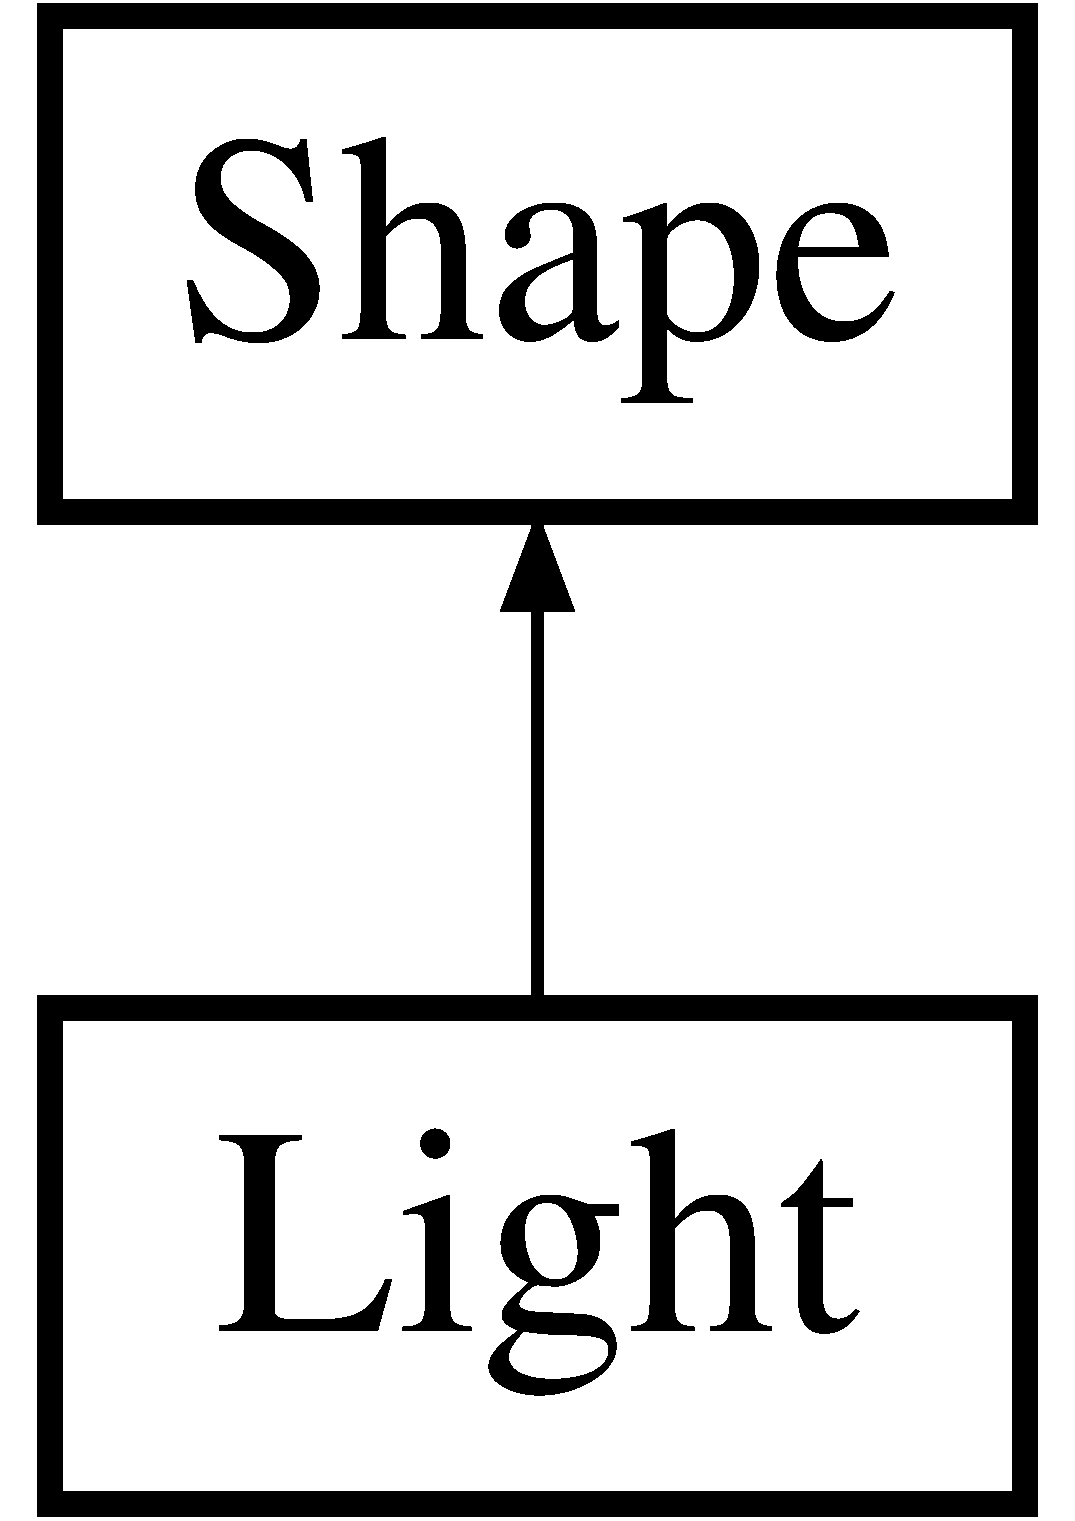
\includegraphics[height=2.000000cm]{classLight}
\end{center}
\end{figure}
\subsection*{Public Member Functions}
\begin{DoxyCompactItemize}
\item 
\hyperlink{classLight_a1e4797b7ed1488b6d6990489f5434c34}{Light} (double x, double y, double w, double l, double sp, double ori, \hyperlink{Shape_8h_a5a4538eeab397888d88a4eefcc5a1345}{Shape\-Type} st, float c\mbox{[}3\mbox{]})
\begin{DoxyCompactList}\small\item\em A Constructor. \end{DoxyCompactList}\item 
\hyperlink{classLight_ad0e59fad13bb6cfadc25b2c477e9ddc7}{$\sim$\-Light} ()
\begin{DoxyCompactList}\small\item\em Default deconstructor. \end{DoxyCompactList}\item 
void \hyperlink{classLight_ac9e3a10f4413cdd83325397e38cd2dbe}{set\-Action\-Range} (double new\-Range)
\begin{DoxyCompactList}\small\item\em set light's action range through arguement. \end{DoxyCompactList}\item 
double \hyperlink{classLight_afe69e219ba4af853ad17408b50147cfe}{get\-Action\-Range} ()
\begin{DoxyCompactList}\small\item\em Return action range of the light. \end{DoxyCompactList}\item 
\hyperlink{Shape_8h_ad4f6886266572e51d198a61a6c762ce5}{Wall} \hyperlink{classLight_a47adb475bd05d17248c28c62c41dbc8a}{detect\-Wall} (double witdth, double height)
\begin{DoxyCompactList}\small\item\em Detect whether light against the wall of window. \end{DoxyCompactList}\end{DoxyCompactItemize}
\subsection*{Private Attributes}
\begin{DoxyCompactItemize}
\item 
double \hyperlink{classLight_ada425b10c6d859e3348165267f19d752}{action\-Range}
\end{DoxyCompactItemize}


\subsection{Detailed Description}
A light class contains attributes and behaviors. 

Inherit from \hyperlink{classShape}{Shape} class, add speed and orientation attributes. 

\subsection{Constructor \& Destructor Documentation}
\hypertarget{classLight_a1e4797b7ed1488b6d6990489f5434c34}{\index{Light@{Light}!Light@{Light}}
\index{Light@{Light}!Light@{Light}}
\subsubsection[{Light}]{\setlength{\rightskip}{0pt plus 5cm}Light\-::\-Light (
\begin{DoxyParamCaption}
\item[{double}]{x, }
\item[{double}]{y, }
\item[{double}]{w, }
\item[{double}]{l, }
\item[{double}]{sp, }
\item[{double}]{ori, }
\item[{{\bf Shape\-Type}}]{st, }
\item[{float}]{c\mbox{[}3\mbox{]}}
\end{DoxyParamCaption}
)}}\label{classLight_a1e4797b7ed1488b6d6990489f5434c34}


A Constructor. 

\begin{DoxyAuthor}{Author}
Zixiao Wang 
\end{DoxyAuthor}

\begin{DoxyParams}{Parameters}
{\em x} & The x position of \hyperlink{classShape}{Shape}. \\
\hline
{\em y} & The y position of \hyperlink{classShape}{Shape}. \\
\hline
{\em w} & The width of \hyperlink{classShape}{Shape}. \\
\hline
{\em l} & The length of \hyperlink{classShape}{Shape}. \\
\hline
{\em sp} & The speed of \hyperlink{classShape}{Shape}. \\
\hline
{\em ori} & The orientation of \hyperlink{classShape}{Shape}. \\
\hline
{\em st} & The Shape\-Type of \hyperlink{classShape}{Shape}. \\
\hline
{\em c} & The color of \hyperlink{classShape}{Shape}. \\
\hline
\end{DoxyParams}
\hypertarget{classLight_ad0e59fad13bb6cfadc25b2c477e9ddc7}{\index{Light@{Light}!$\sim$\-Light@{$\sim$\-Light}}
\index{$\sim$\-Light@{$\sim$\-Light}!Light@{Light}}
\subsubsection[{$\sim$\-Light}]{\setlength{\rightskip}{0pt plus 5cm}Light\-::$\sim$\-Light (
\begin{DoxyParamCaption}
{}
\end{DoxyParamCaption}
)}}\label{classLight_ad0e59fad13bb6cfadc25b2c477e9ddc7}


Default deconstructor. 

\begin{DoxyAuthor}{Author}
Zixiao Wang 
\end{DoxyAuthor}


\subsection{Member Function Documentation}
\hypertarget{classLight_a47adb475bd05d17248c28c62c41dbc8a}{\index{Light@{Light}!detect\-Wall@{detect\-Wall}}
\index{detect\-Wall@{detect\-Wall}!Light@{Light}}
\subsubsection[{detect\-Wall}]{\setlength{\rightskip}{0pt plus 5cm}{\bf Wall} Light\-::detect\-Wall (
\begin{DoxyParamCaption}
\item[{double}]{witdth, }
\item[{double}]{height}
\end{DoxyParamCaption}
)}}\label{classLight_a47adb475bd05d17248c28c62c41dbc8a}


Detect whether light against the wall of window. 

\begin{DoxyAuthor}{Author}
Zixiao Wang 
\end{DoxyAuthor}

\begin{DoxyParams}{Parameters}
{\em width} & The witdth of window(default\-: 800) \\
\hline
{\em height} & The height of window(default\-: 800) \\
\hline
\end{DoxyParams}
\hypertarget{classLight_afe69e219ba4af853ad17408b50147cfe}{\index{Light@{Light}!get\-Action\-Range@{get\-Action\-Range}}
\index{get\-Action\-Range@{get\-Action\-Range}!Light@{Light}}
\subsubsection[{get\-Action\-Range}]{\setlength{\rightskip}{0pt plus 5cm}double Light\-::get\-Action\-Range (
\begin{DoxyParamCaption}
{}
\end{DoxyParamCaption}
)}}\label{classLight_afe69e219ba4af853ad17408b50147cfe}


Return action range of the light. 

\begin{DoxyAuthor}{Author}
Zixiao Wang 
\end{DoxyAuthor}
\hypertarget{classLight_ac9e3a10f4413cdd83325397e38cd2dbe}{\index{Light@{Light}!set\-Action\-Range@{set\-Action\-Range}}
\index{set\-Action\-Range@{set\-Action\-Range}!Light@{Light}}
\subsubsection[{set\-Action\-Range}]{\setlength{\rightskip}{0pt plus 5cm}void Light\-::set\-Action\-Range (
\begin{DoxyParamCaption}
\item[{double}]{new\-Range}
\end{DoxyParamCaption}
)}}\label{classLight_ac9e3a10f4413cdd83325397e38cd2dbe}


set light's action range through arguement. 

\begin{DoxyAuthor}{Author}
Zixiao Wang 
\end{DoxyAuthor}

\begin{DoxyParams}{Parameters}
{\em new\-Sensor\-Type} & Set \hyperlink{classLight}{Light}'s action range according to arguement new\-Range. \\
\hline
\end{DoxyParams}


\subsection{Member Data Documentation}
\hypertarget{classLight_ada425b10c6d859e3348165267f19d752}{\index{Light@{Light}!action\-Range@{action\-Range}}
\index{action\-Range@{action\-Range}!Light@{Light}}
\subsubsection[{action\-Range}]{\setlength{\rightskip}{0pt plus 5cm}double Light\-::action\-Range\hspace{0.3cm}{\ttfamily [private]}}}\label{classLight_ada425b10c6d859e3348165267f19d752}
The action range of light 

The documentation for this class was generated from the following files\-:\begin{DoxyCompactItemize}
\item 
\hyperlink{Light_8h}{Light.\-h}\item 
\hyperlink{Light_8cpp}{Light.\-cpp}\end{DoxyCompactItemize}

\hypertarget{classRobotClass}{\section{Robot\-Class Class Reference}
\label{classRobotClass}\index{Robot\-Class@{Robot\-Class}}
}


A robot class contains attributes and hehaviors.  




{\ttfamily \#include $<$Robot\-Class.\-h$>$}

Inheritance diagram for Robot\-Class\-:\begin{figure}[H]
\begin{center}
\leavevmode
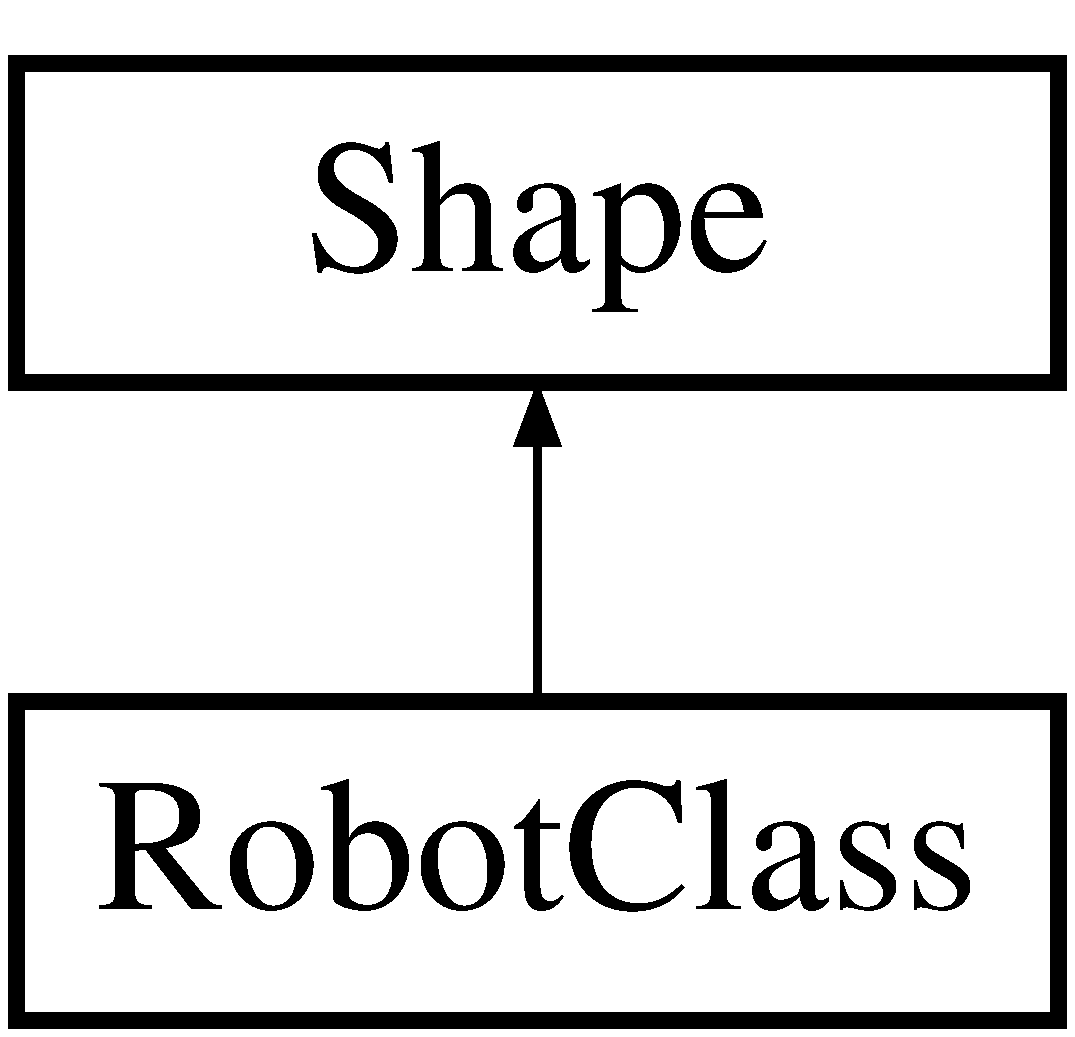
\includegraphics[height=2.000000cm]{classRobotClass}
\end{center}
\end{figure}
\subsection*{Public Member Functions}
\begin{DoxyCompactItemize}
\item 
\hyperlink{classRobotClass_a7125604039c2a4b39e34e4354bd4ce19}{Robot\-Class} ()
\begin{DoxyCompactList}\small\item\em The default constructor. \end{DoxyCompactList}\item 
\hyperlink{classRobotClass_ab91816f1d752646bc82cc20f9710a107}{Robot\-Class} (double x, double y, double w, double l, double sp, double ori, \hyperlink{Shape_8h_a5a4538eeab397888d88a4eefcc5a1345}{Shape\-Type} \hyperlink{classShape_a18af04fdf7a9e121518f3c7278693c60}{shape\-Type}, float c\mbox{[}3\mbox{]}, \hyperlink{Sensor_8h_aa1f0e2efd52935fd01bfece0fbead81f}{Connection\-Type} ct, int id)
\begin{DoxyCompactList}\small\item\em A Constructor. \end{DoxyCompactList}\item 
\hyperlink{classRobotClass_a7d7725737f146f85ed7ceeae7f300e9e}{$\sim$\-Robot\-Class} ()
\begin{DoxyCompactList}\small\item\em Default deconstructor. \end{DoxyCompactList}\item 
void \hyperlink{classRobotClass_a583bdc55d13af3e8bd11f89d783455c0}{set\-I\-D} (int id)
\begin{DoxyCompactList}\small\item\em set robot's I\-D through arguement. \end{DoxyCompactList}\item 
void \hyperlink{classRobotClass_aaa965d250757f64738c66387791a6263}{set\-Connection\-Type} (\hyperlink{Sensor_8h_aa1f0e2efd52935fd01bfece0fbead81f}{Connection\-Type} newconnection\-Type)
\begin{DoxyCompactList}\small\item\em set Robot's Connection\-Type through arguement. \end{DoxyCompactList}\item 
void \hyperlink{classRobotClass_a7debd529fda1f510830328cf873cbc63}{set\-Left\-Speed} (double sp)
\begin{DoxyCompactList}\small\item\em set Robot's left wheel speed. \end{DoxyCompactList}\item 
void \hyperlink{classRobotClass_a202a15a9709496ca9736094af0e84ecc}{set\-Right\-Speed} (double sp)
\begin{DoxyCompactList}\small\item\em set Robot's right wheel speed. \end{DoxyCompactList}\item 
void \hyperlink{classRobotClass_a819a477d23d1c54d2094a477feed8477}{set\-Left\-Wheel\-Position} (double x, double y)
\begin{DoxyCompactList}\small\item\em set Robot's left wheel position. \end{DoxyCompactList}\item 
void \hyperlink{classRobotClass_ac72404efc5f43d9e25bcd2190a987cc5}{set\-Right\-Wheel\-Position} (double x, double y)
\begin{DoxyCompactList}\small\item\em set Robot's right wheel x position. \end{DoxyCompactList}\item 
void \hyperlink{classRobotClass_ac5980c62b0fa569360e12dc066da98a4}{set\-New\-Position} (double x, double y)
\begin{DoxyCompactList}\small\item\em set Robot's position, according to left wheel and right wheel. \end{DoxyCompactList}\item 
void \hyperlink{classRobotClass_a348207c6b74eeff725c5f329f0579482}{set\-Action\-Range} (double ar)
\begin{DoxyCompactList}\small\item\em set Robot's action range, according to input. \end{DoxyCompactList}\item 
int \hyperlink{classRobotClass_a6b817a39e292edf591c65a68a31a3012}{get\-I\-D} ()
\begin{DoxyCompactList}\small\item\em Return I\-D of robot. \end{DoxyCompactList}\item 
double \hyperlink{classRobotClass_aa37142a222c6b2fc1f877d395f0b371d}{get\-Left\-Speed} ()
\begin{DoxyCompactList}\small\item\em Return leftspeed of robot. \end{DoxyCompactList}\item 
double \hyperlink{classRobotClass_ab414f4d538c9ba99c32c0297ac8ca189}{get\-Right\-Speed} ()
\begin{DoxyCompactList}\small\item\em Return rightspeed of robot. \end{DoxyCompactList}\item 
double \hyperlink{classRobotClass_a3fc92ded2588d8e880be8301fe7e78ca}{get\-Left\-Wheel\-X} ()
\begin{DoxyCompactList}\small\item\em Return Left\-Wheel\-X of robot. \end{DoxyCompactList}\item 
double \hyperlink{classRobotClass_ab6d7104d418020f8a1d7254700eead0e}{get\-Left\-Wheel\-Y} ()
\begin{DoxyCompactList}\small\item\em Return Left\-Wheel\-Y of robot. \end{DoxyCompactList}\item 
double \hyperlink{classRobotClass_a5d32eb96cbb3bfe01b956f09e35b925c}{get\-Right\-Wheel\-X} ()
\begin{DoxyCompactList}\small\item\em Return Right\-Wheel\-X of robot. \end{DoxyCompactList}\item 
double \hyperlink{classRobotClass_abc35edf633f6b03a0956e2bdb68a127c}{get\-Right\-Wheel\-Y} ()
\begin{DoxyCompactList}\small\item\em Return Right\-Wheel\-Y of robot. \end{DoxyCompactList}\item 
\hyperlink{Sensor_8h_aa1f0e2efd52935fd01bfece0fbead81f}{Connection\-Type} \hyperlink{classRobotClass_ad1f430d26cf7265285db0742a0fd6f34}{get\-Connection\-Type} ()
\begin{DoxyCompactList}\small\item\em Return connection type of Robot. \end{DoxyCompactList}\item 
double \hyperlink{classRobotClass_a37170c1d224daa872fb4a506719bb43f}{get\-Action\-Range} ()
\begin{DoxyCompactList}\small\item\em Return action range of Robot. \end{DoxyCompactList}\item 
\hyperlink{Shape_8h_ad4f6886266572e51d198a61a6c762ce5}{Wall} \hyperlink{classRobotClass_a3a660d9392490322535d0dda4fa27f27}{detect\-Wall} (double witdth, double height)
\begin{DoxyCompactList}\small\item\em Detect whether robot against the wall of window. \end{DoxyCompactList}\item 
void \hyperlink{classRobotClass_a111ff5cb11fb67bf3cae0797d955e24a}{detect\-Stimulation} (std\-::vector$<$ \hyperlink{classRobotClass}{Robot\-Class} $>$ robots, std\-::vector$<$ \hyperlink{classLight}{Light} $>$ lights, double stimulation\mbox{[}2\mbox{]})
\begin{DoxyCompactList}\small\item\em Detect whether robot against obstacle. \end{DoxyCompactList}\end{DoxyCompactItemize}
\subsection*{Private Attributes}
\begin{DoxyCompactItemize}
\item 
std\-::vector$<$ \hyperlink{classSensor}{Sensor} $>$ \hyperlink{classRobotClass_ab9fae941de661646a5dbc9758e86306d}{sensors}
\item 
std\-::vector$<$ \hyperlink{classWheel}{Wheel} $>$ \hyperlink{classRobotClass_a52934dab5fdec48b101ad0c71fb60e48}{wheels}
\item 
int \hyperlink{classRobotClass_afccead30da94de14c11e2305c33991f2}{I\-D}
\item 
\hyperlink{Sensor_8h_aa1f0e2efd52935fd01bfece0fbead81f}{Connection\-Type} \hyperlink{classRobotClass_a073b0cd68ebfd906f9dc42029e04d1fe}{connection\-Type}
\item 
double \hyperlink{classRobotClass_a009553675263e4e281305051f9afc2ba}{action\-Range}
\end{DoxyCompactItemize}


\subsection{Detailed Description}
A robot class contains attributes and hehaviors. 

Inherit from \hyperlink{classShape}{Shape} class, add speed and orientation attributes. 

\subsection{Constructor \& Destructor Documentation}
\hypertarget{classRobotClass_a7125604039c2a4b39e34e4354bd4ce19}{\index{Robot\-Class@{Robot\-Class}!Robot\-Class@{Robot\-Class}}
\index{Robot\-Class@{Robot\-Class}!RobotClass@{Robot\-Class}}
\subsubsection[{Robot\-Class}]{\setlength{\rightskip}{0pt plus 5cm}Robot\-Class\-::\-Robot\-Class (
\begin{DoxyParamCaption}
{}
\end{DoxyParamCaption}
)}}\label{classRobotClass_a7125604039c2a4b39e34e4354bd4ce19}


The default constructor. 

\hypertarget{classRobotClass_ab91816f1d752646bc82cc20f9710a107}{\index{Robot\-Class@{Robot\-Class}!Robot\-Class@{Robot\-Class}}
\index{Robot\-Class@{Robot\-Class}!RobotClass@{Robot\-Class}}
\subsubsection[{Robot\-Class}]{\setlength{\rightskip}{0pt plus 5cm}Robot\-Class\-::\-Robot\-Class (
\begin{DoxyParamCaption}
\item[{double}]{x, }
\item[{double}]{y, }
\item[{double}]{w, }
\item[{double}]{l, }
\item[{double}]{sp, }
\item[{double}]{ori, }
\item[{{\bf Shape\-Type}}]{shape\-Type, }
\item[{float}]{c\mbox{[}3\mbox{]}, }
\item[{{\bf Connection\-Type}}]{ct, }
\item[{int}]{id}
\end{DoxyParamCaption}
)}}\label{classRobotClass_ab91816f1d752646bc82cc20f9710a107}


A Constructor. 

\begin{DoxyAuthor}{Author}
Zixiao Wang 
\end{DoxyAuthor}

\begin{DoxyParams}{Parameters}
{\em x} & The x position of robot. \\
\hline
{\em y} & The y position of robot. \\
\hline
{\em w} & The width of robot. \\
\hline
{\em l} & The length of robot. \\
\hline
{\em sp} & The speed of robot. \\
\hline
{\em ori} & The orientation of robot. \\
\hline
{\em shape\-Type} & The shape type of robot. \\
\hline
{\em c} & The color of robot. \\
\hline
{\em ct} & The connection type of robot. \\
\hline
{\em id} & The id of robot. \\
\hline
\end{DoxyParams}
\hypertarget{classRobotClass_a7d7725737f146f85ed7ceeae7f300e9e}{\index{Robot\-Class@{Robot\-Class}!$\sim$\-Robot\-Class@{$\sim$\-Robot\-Class}}
\index{$\sim$\-Robot\-Class@{$\sim$\-Robot\-Class}!RobotClass@{Robot\-Class}}
\subsubsection[{$\sim$\-Robot\-Class}]{\setlength{\rightskip}{0pt plus 5cm}Robot\-Class\-::$\sim$\-Robot\-Class (
\begin{DoxyParamCaption}
{}
\end{DoxyParamCaption}
)}}\label{classRobotClass_a7d7725737f146f85ed7ceeae7f300e9e}


Default deconstructor. 

\begin{DoxyAuthor}{Author}
Zixiao Wang 
\end{DoxyAuthor}


\subsection{Member Function Documentation}
\hypertarget{classRobotClass_a111ff5cb11fb67bf3cae0797d955e24a}{\index{Robot\-Class@{Robot\-Class}!detect\-Stimulation@{detect\-Stimulation}}
\index{detect\-Stimulation@{detect\-Stimulation}!RobotClass@{Robot\-Class}}
\subsubsection[{detect\-Stimulation}]{\setlength{\rightskip}{0pt plus 5cm}void Robot\-Class\-::detect\-Stimulation (
\begin{DoxyParamCaption}
\item[{std\-::vector$<$ {\bf Robot\-Class} $>$}]{robots, }
\item[{std\-::vector$<$ {\bf Light} $>$}]{lights, }
\item[{double}]{stimulation\mbox{[}2\mbox{]}}
\end{DoxyParamCaption}
)}}\label{classRobotClass_a111ff5cb11fb67bf3cae0797d955e24a}


Detect whether robot against obstacle. 

\begin{DoxyAuthor}{Author}
Zixiao Wang 
\end{DoxyAuthor}

\begin{DoxyParams}{Parameters}
{\em obs} & Obstacle that used to detect whether there is a collision \\
\hline
\end{DoxyParams}
\hypertarget{classRobotClass_a3a660d9392490322535d0dda4fa27f27}{\index{Robot\-Class@{Robot\-Class}!detect\-Wall@{detect\-Wall}}
\index{detect\-Wall@{detect\-Wall}!RobotClass@{Robot\-Class}}
\subsubsection[{detect\-Wall}]{\setlength{\rightskip}{0pt plus 5cm}{\bf Wall} Robot\-Class\-::detect\-Wall (
\begin{DoxyParamCaption}
\item[{double}]{witdth, }
\item[{double}]{height}
\end{DoxyParamCaption}
)}}\label{classRobotClass_a3a660d9392490322535d0dda4fa27f27}


Detect whether robot against the wall of window. 

\begin{DoxyAuthor}{Author}
Triny Chen and Zixiao Wang 
\end{DoxyAuthor}

\begin{DoxyParams}{Parameters}
{\em width} & The witdth of window(default\-: 800) \\
\hline
{\em height} & The height of window(default\-: 800) \\
\hline
\end{DoxyParams}
\hypertarget{classRobotClass_a37170c1d224daa872fb4a506719bb43f}{\index{Robot\-Class@{Robot\-Class}!get\-Action\-Range@{get\-Action\-Range}}
\index{get\-Action\-Range@{get\-Action\-Range}!RobotClass@{Robot\-Class}}
\subsubsection[{get\-Action\-Range}]{\setlength{\rightskip}{0pt plus 5cm}double Robot\-Class\-::get\-Action\-Range (
\begin{DoxyParamCaption}
{}
\end{DoxyParamCaption}
)}}\label{classRobotClass_a37170c1d224daa872fb4a506719bb43f}


Return action range of Robot. 

\begin{DoxyAuthor}{Author}
Zixiao Wang 
\end{DoxyAuthor}
\hypertarget{classRobotClass_ad1f430d26cf7265285db0742a0fd6f34}{\index{Robot\-Class@{Robot\-Class}!get\-Connection\-Type@{get\-Connection\-Type}}
\index{get\-Connection\-Type@{get\-Connection\-Type}!RobotClass@{Robot\-Class}}
\subsubsection[{get\-Connection\-Type}]{\setlength{\rightskip}{0pt plus 5cm}{\bf Connection\-Type} Robot\-Class\-::get\-Connection\-Type (
\begin{DoxyParamCaption}
{}
\end{DoxyParamCaption}
)}}\label{classRobotClass_ad1f430d26cf7265285db0742a0fd6f34}


Return connection type of Robot. 

\begin{DoxyAuthor}{Author}
Zixiao Wang 
\end{DoxyAuthor}
\hypertarget{classRobotClass_a6b817a39e292edf591c65a68a31a3012}{\index{Robot\-Class@{Robot\-Class}!get\-I\-D@{get\-I\-D}}
\index{get\-I\-D@{get\-I\-D}!RobotClass@{Robot\-Class}}
\subsubsection[{get\-I\-D}]{\setlength{\rightskip}{0pt plus 5cm}int Robot\-Class\-::get\-I\-D (
\begin{DoxyParamCaption}
{}
\end{DoxyParamCaption}
)}}\label{classRobotClass_a6b817a39e292edf591c65a68a31a3012}


Return I\-D of robot. 

\begin{DoxyAuthor}{Author}
Zixiao Wang 
\end{DoxyAuthor}
\hypertarget{classRobotClass_aa37142a222c6b2fc1f877d395f0b371d}{\index{Robot\-Class@{Robot\-Class}!get\-Left\-Speed@{get\-Left\-Speed}}
\index{get\-Left\-Speed@{get\-Left\-Speed}!RobotClass@{Robot\-Class}}
\subsubsection[{get\-Left\-Speed}]{\setlength{\rightskip}{0pt plus 5cm}double Robot\-Class\-::get\-Left\-Speed (
\begin{DoxyParamCaption}
{}
\end{DoxyParamCaption}
)}}\label{classRobotClass_aa37142a222c6b2fc1f877d395f0b371d}


Return leftspeed of robot. 

\begin{DoxyAuthor}{Author}
Yangyun Li 
\end{DoxyAuthor}
\hypertarget{classRobotClass_a3fc92ded2588d8e880be8301fe7e78ca}{\index{Robot\-Class@{Robot\-Class}!get\-Left\-Wheel\-X@{get\-Left\-Wheel\-X}}
\index{get\-Left\-Wheel\-X@{get\-Left\-Wheel\-X}!RobotClass@{Robot\-Class}}
\subsubsection[{get\-Left\-Wheel\-X}]{\setlength{\rightskip}{0pt plus 5cm}double Robot\-Class\-::get\-Left\-Wheel\-X (
\begin{DoxyParamCaption}
{}
\end{DoxyParamCaption}
)}}\label{classRobotClass_a3fc92ded2588d8e880be8301fe7e78ca}


Return Left\-Wheel\-X of robot. 

\begin{DoxyAuthor}{Author}
Yangyun Li 
\end{DoxyAuthor}
\hypertarget{classRobotClass_ab6d7104d418020f8a1d7254700eead0e}{\index{Robot\-Class@{Robot\-Class}!get\-Left\-Wheel\-Y@{get\-Left\-Wheel\-Y}}
\index{get\-Left\-Wheel\-Y@{get\-Left\-Wheel\-Y}!RobotClass@{Robot\-Class}}
\subsubsection[{get\-Left\-Wheel\-Y}]{\setlength{\rightskip}{0pt plus 5cm}double Robot\-Class\-::get\-Left\-Wheel\-Y (
\begin{DoxyParamCaption}
{}
\end{DoxyParamCaption}
)}}\label{classRobotClass_ab6d7104d418020f8a1d7254700eead0e}


Return Left\-Wheel\-Y of robot. 

\begin{DoxyAuthor}{Author}
Yangyun Li 
\end{DoxyAuthor}
\hypertarget{classRobotClass_ab414f4d538c9ba99c32c0297ac8ca189}{\index{Robot\-Class@{Robot\-Class}!get\-Right\-Speed@{get\-Right\-Speed}}
\index{get\-Right\-Speed@{get\-Right\-Speed}!RobotClass@{Robot\-Class}}
\subsubsection[{get\-Right\-Speed}]{\setlength{\rightskip}{0pt plus 5cm}double Robot\-Class\-::get\-Right\-Speed (
\begin{DoxyParamCaption}
{}
\end{DoxyParamCaption}
)}}\label{classRobotClass_ab414f4d538c9ba99c32c0297ac8ca189}


Return rightspeed of robot. 

\begin{DoxyAuthor}{Author}
Yangyun Li 
\end{DoxyAuthor}
\hypertarget{classRobotClass_a5d32eb96cbb3bfe01b956f09e35b925c}{\index{Robot\-Class@{Robot\-Class}!get\-Right\-Wheel\-X@{get\-Right\-Wheel\-X}}
\index{get\-Right\-Wheel\-X@{get\-Right\-Wheel\-X}!RobotClass@{Robot\-Class}}
\subsubsection[{get\-Right\-Wheel\-X}]{\setlength{\rightskip}{0pt plus 5cm}double Robot\-Class\-::get\-Right\-Wheel\-X (
\begin{DoxyParamCaption}
{}
\end{DoxyParamCaption}
)}}\label{classRobotClass_a5d32eb96cbb3bfe01b956f09e35b925c}


Return Right\-Wheel\-X of robot. 

\begin{DoxyAuthor}{Author}
Yangyun Li 
\end{DoxyAuthor}
\hypertarget{classRobotClass_abc35edf633f6b03a0956e2bdb68a127c}{\index{Robot\-Class@{Robot\-Class}!get\-Right\-Wheel\-Y@{get\-Right\-Wheel\-Y}}
\index{get\-Right\-Wheel\-Y@{get\-Right\-Wheel\-Y}!RobotClass@{Robot\-Class}}
\subsubsection[{get\-Right\-Wheel\-Y}]{\setlength{\rightskip}{0pt plus 5cm}double Robot\-Class\-::get\-Right\-Wheel\-Y (
\begin{DoxyParamCaption}
{}
\end{DoxyParamCaption}
)}}\label{classRobotClass_abc35edf633f6b03a0956e2bdb68a127c}


Return Right\-Wheel\-Y of robot. 

\begin{DoxyAuthor}{Author}
Yangyun Li 
\end{DoxyAuthor}
\hypertarget{classRobotClass_a348207c6b74eeff725c5f329f0579482}{\index{Robot\-Class@{Robot\-Class}!set\-Action\-Range@{set\-Action\-Range}}
\index{set\-Action\-Range@{set\-Action\-Range}!RobotClass@{Robot\-Class}}
\subsubsection[{set\-Action\-Range}]{\setlength{\rightskip}{0pt plus 5cm}void Robot\-Class\-::set\-Action\-Range (
\begin{DoxyParamCaption}
\item[{double}]{ar}
\end{DoxyParamCaption}
)}}\label{classRobotClass_a348207c6b74eeff725c5f329f0579482}


set Robot's action range, according to input. 

\begin{DoxyAuthor}{Author}
Zixiao Wang 
\end{DoxyAuthor}
\hypertarget{classRobotClass_aaa965d250757f64738c66387791a6263}{\index{Robot\-Class@{Robot\-Class}!set\-Connection\-Type@{set\-Connection\-Type}}
\index{set\-Connection\-Type@{set\-Connection\-Type}!RobotClass@{Robot\-Class}}
\subsubsection[{set\-Connection\-Type}]{\setlength{\rightskip}{0pt plus 5cm}void Robot\-Class\-::set\-Connection\-Type (
\begin{DoxyParamCaption}
\item[{{\bf Connection\-Type}}]{newconnection\-Type}
\end{DoxyParamCaption}
)}}\label{classRobotClass_aaa965d250757f64738c66387791a6263}


set Robot's Connection\-Type through arguement. 

\begin{DoxyAuthor}{Author}
Zixiao Wang 
\end{DoxyAuthor}

\begin{DoxyParams}{Parameters}
{\em newconnection\-Type} & Set Robot's connection\-Type according to arguement newconnection\-Type. \\
\hline
\end{DoxyParams}
\hypertarget{classRobotClass_a583bdc55d13af3e8bd11f89d783455c0}{\index{Robot\-Class@{Robot\-Class}!set\-I\-D@{set\-I\-D}}
\index{set\-I\-D@{set\-I\-D}!RobotClass@{Robot\-Class}}
\subsubsection[{set\-I\-D}]{\setlength{\rightskip}{0pt plus 5cm}void Robot\-Class\-::set\-I\-D (
\begin{DoxyParamCaption}
\item[{int}]{id}
\end{DoxyParamCaption}
)}}\label{classRobotClass_a583bdc55d13af3e8bd11f89d783455c0}


set robot's I\-D through arguement. 

\begin{DoxyAuthor}{Author}
Zixiao Wang 
\end{DoxyAuthor}

\begin{DoxyParams}{Parameters}
{\em new\-Wheel\-I\-D} & Set robot's I\-D according to arguement id. \\
\hline
\end{DoxyParams}
\hypertarget{classRobotClass_a7debd529fda1f510830328cf873cbc63}{\index{Robot\-Class@{Robot\-Class}!set\-Left\-Speed@{set\-Left\-Speed}}
\index{set\-Left\-Speed@{set\-Left\-Speed}!RobotClass@{Robot\-Class}}
\subsubsection[{set\-Left\-Speed}]{\setlength{\rightskip}{0pt plus 5cm}void Robot\-Class\-::set\-Left\-Speed (
\begin{DoxyParamCaption}
\item[{double}]{sp}
\end{DoxyParamCaption}
)}}\label{classRobotClass_a7debd529fda1f510830328cf873cbc63}


set Robot's left wheel speed. 

\begin{DoxyAuthor}{Author}
Yangyun Li 
\end{DoxyAuthor}
\hypertarget{classRobotClass_a819a477d23d1c54d2094a477feed8477}{\index{Robot\-Class@{Robot\-Class}!set\-Left\-Wheel\-Position@{set\-Left\-Wheel\-Position}}
\index{set\-Left\-Wheel\-Position@{set\-Left\-Wheel\-Position}!RobotClass@{Robot\-Class}}
\subsubsection[{set\-Left\-Wheel\-Position}]{\setlength{\rightskip}{0pt plus 5cm}void Robot\-Class\-::set\-Left\-Wheel\-Position (
\begin{DoxyParamCaption}
\item[{double}]{x, }
\item[{double}]{y}
\end{DoxyParamCaption}
)}}\label{classRobotClass_a819a477d23d1c54d2094a477feed8477}


set Robot's left wheel position. 

\begin{DoxyAuthor}{Author}
Yangyun Li 
\end{DoxyAuthor}
\hypertarget{classRobotClass_ac5980c62b0fa569360e12dc066da98a4}{\index{Robot\-Class@{Robot\-Class}!set\-New\-Position@{set\-New\-Position}}
\index{set\-New\-Position@{set\-New\-Position}!RobotClass@{Robot\-Class}}
\subsubsection[{set\-New\-Position}]{\setlength{\rightskip}{0pt plus 5cm}void Robot\-Class\-::set\-New\-Position (
\begin{DoxyParamCaption}
\item[{double}]{x, }
\item[{double}]{y}
\end{DoxyParamCaption}
)}}\label{classRobotClass_ac5980c62b0fa569360e12dc066da98a4}


set Robot's position, according to left wheel and right wheel. 

\begin{DoxyAuthor}{Author}
Zixiao Wang 
\end{DoxyAuthor}
\hypertarget{classRobotClass_a202a15a9709496ca9736094af0e84ecc}{\index{Robot\-Class@{Robot\-Class}!set\-Right\-Speed@{set\-Right\-Speed}}
\index{set\-Right\-Speed@{set\-Right\-Speed}!RobotClass@{Robot\-Class}}
\subsubsection[{set\-Right\-Speed}]{\setlength{\rightskip}{0pt plus 5cm}void Robot\-Class\-::set\-Right\-Speed (
\begin{DoxyParamCaption}
\item[{double}]{sp}
\end{DoxyParamCaption}
)}}\label{classRobotClass_a202a15a9709496ca9736094af0e84ecc}


set Robot's right wheel speed. 

\begin{DoxyAuthor}{Author}
Yangyun Li 
\end{DoxyAuthor}
\hypertarget{classRobotClass_ac72404efc5f43d9e25bcd2190a987cc5}{\index{Robot\-Class@{Robot\-Class}!set\-Right\-Wheel\-Position@{set\-Right\-Wheel\-Position}}
\index{set\-Right\-Wheel\-Position@{set\-Right\-Wheel\-Position}!RobotClass@{Robot\-Class}}
\subsubsection[{set\-Right\-Wheel\-Position}]{\setlength{\rightskip}{0pt plus 5cm}void Robot\-Class\-::set\-Right\-Wheel\-Position (
\begin{DoxyParamCaption}
\item[{double}]{x, }
\item[{double}]{y}
\end{DoxyParamCaption}
)}}\label{classRobotClass_ac72404efc5f43d9e25bcd2190a987cc5}


set Robot's right wheel x position. 

\begin{DoxyAuthor}{Author}
Yangyun Li 
\end{DoxyAuthor}


\subsection{Member Data Documentation}
\hypertarget{classRobotClass_a009553675263e4e281305051f9afc2ba}{\index{Robot\-Class@{Robot\-Class}!action\-Range@{action\-Range}}
\index{action\-Range@{action\-Range}!RobotClass@{Robot\-Class}}
\subsubsection[{action\-Range}]{\setlength{\rightskip}{0pt plus 5cm}double Robot\-Class\-::action\-Range\hspace{0.3cm}{\ttfamily [private]}}}\label{classRobotClass_a009553675263e4e281305051f9afc2ba}
Action range of robot \hypertarget{classRobotClass_a073b0cd68ebfd906f9dc42029e04d1fe}{\index{Robot\-Class@{Robot\-Class}!connection\-Type@{connection\-Type}}
\index{connection\-Type@{connection\-Type}!RobotClass@{Robot\-Class}}
\subsubsection[{connection\-Type}]{\setlength{\rightskip}{0pt plus 5cm}{\bf Connection\-Type} Robot\-Class\-::connection\-Type\hspace{0.3cm}{\ttfamily [private]}}}\label{classRobotClass_a073b0cd68ebfd906f9dc42029e04d1fe}
Connecntion type of robot \hypertarget{classRobotClass_afccead30da94de14c11e2305c33991f2}{\index{Robot\-Class@{Robot\-Class}!I\-D@{I\-D}}
\index{I\-D@{I\-D}!RobotClass@{Robot\-Class}}
\subsubsection[{I\-D}]{\setlength{\rightskip}{0pt plus 5cm}int Robot\-Class\-::\-I\-D\hspace{0.3cm}{\ttfamily [private]}}}\label{classRobotClass_afccead30da94de14c11e2305c33991f2}
I\-D of robot \hypertarget{classRobotClass_ab9fae941de661646a5dbc9758e86306d}{\index{Robot\-Class@{Robot\-Class}!sensors@{sensors}}
\index{sensors@{sensors}!RobotClass@{Robot\-Class}}
\subsubsection[{sensors}]{\setlength{\rightskip}{0pt plus 5cm}std\-::vector$<${\bf Sensor}$>$ Robot\-Class\-::sensors\hspace{0.3cm}{\ttfamily [private]}}}\label{classRobotClass_ab9fae941de661646a5dbc9758e86306d}
speed of robot \hypertarget{classRobotClass_a52934dab5fdec48b101ad0c71fb60e48}{\index{Robot\-Class@{Robot\-Class}!wheels@{wheels}}
\index{wheels@{wheels}!RobotClass@{Robot\-Class}}
\subsubsection[{wheels}]{\setlength{\rightskip}{0pt plus 5cm}std\-::vector$<${\bf Wheel}$>$ Robot\-Class\-::wheels\hspace{0.3cm}{\ttfamily [private]}}}\label{classRobotClass_a52934dab5fdec48b101ad0c71fb60e48}
orientation of robot 

The documentation for this class was generated from the following files\-:\begin{DoxyCompactItemize}
\item 
\hyperlink{RobotClass_8h}{Robot\-Class.\-h}\item 
\hyperlink{RobotClass_8cpp}{Robot\-Class.\-cpp}\end{DoxyCompactItemize}

\hypertarget{classSensor}{\section{Sensor Class Reference}
\label{classSensor}\index{Sensor@{Sensor}}
}


{\ttfamily \#include $<$Sensor.\-h$>$}

Inheritance diagram for Sensor\-:\begin{figure}[H]
\begin{center}
\leavevmode
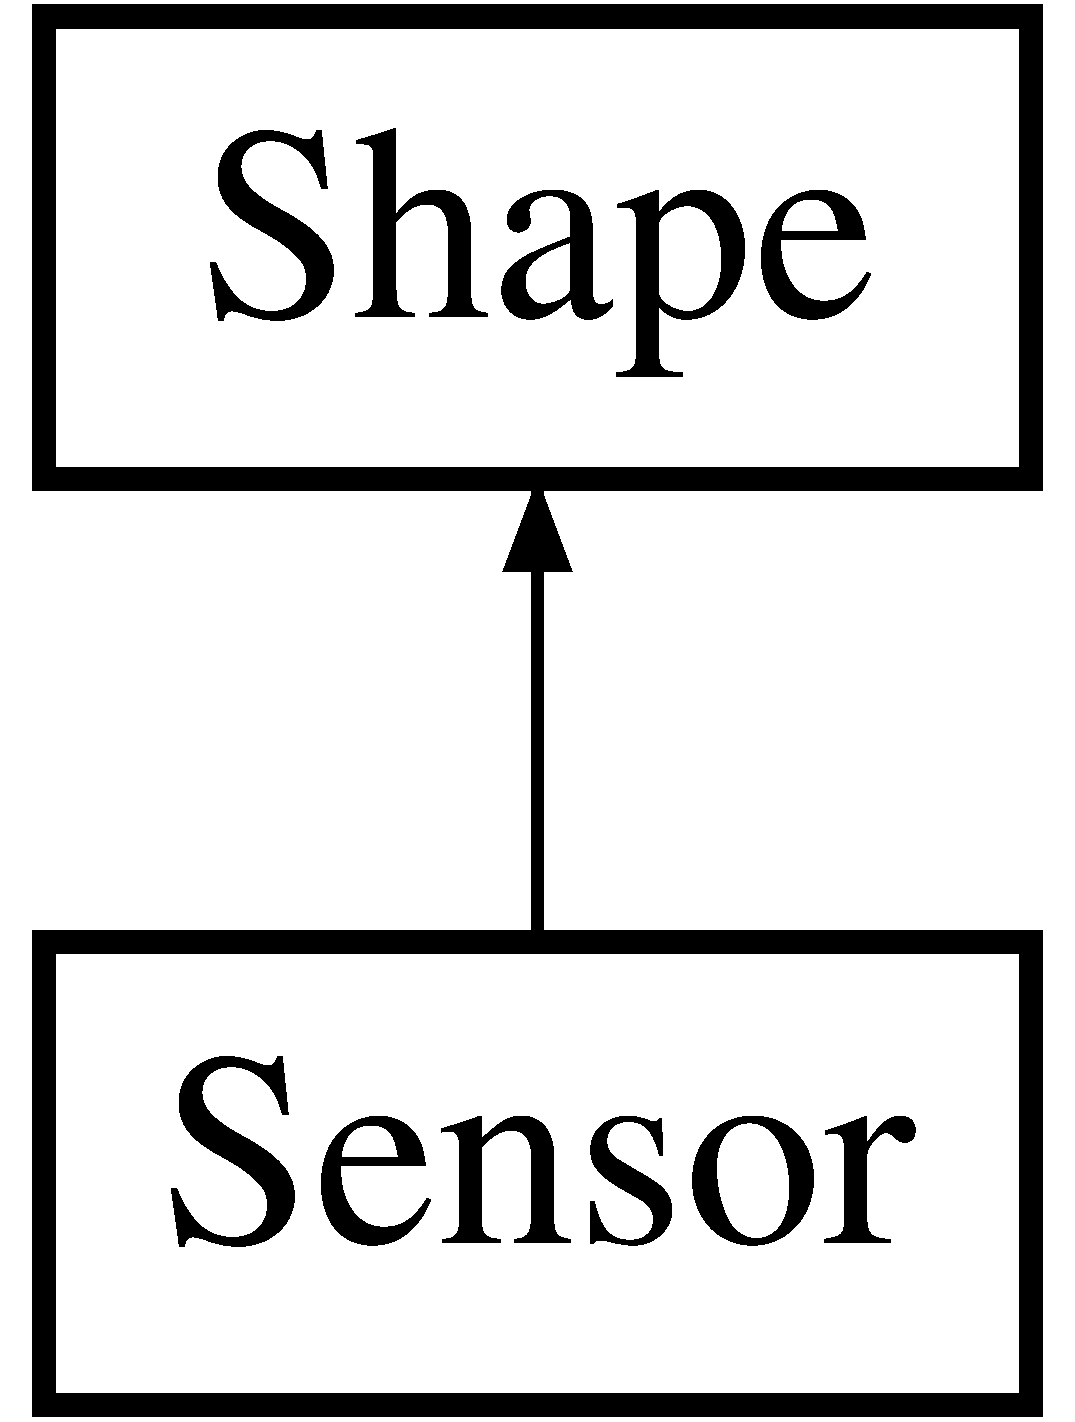
\includegraphics[height=2.000000cm]{classSensor}
\end{center}
\end{figure}
\subsection*{Public Member Functions}
\begin{DoxyCompactItemize}
\item 
\hyperlink{classSensor_a342d6d11ef572c8cba92cb76fb1a294b}{Sensor} ()
\begin{DoxyCompactList}\small\item\em The default constructor. \end{DoxyCompactList}\item 
\hyperlink{classSensor_a44bc63370538b343bcf1cf124f995a12}{Sensor} (double x, double y, double w, double l, double sp, double ori, \hyperlink{Shape_8h_a5a4538eeab397888d88a4eefcc5a1345}{Shape\-Type} st, float c\mbox{[}3\mbox{]}, \hyperlink{Sensor_8h_a213c434cb928c4ca22513e2302632435}{Sensor\-Type} sensort, \hyperlink{Sensor_8h_aa1f0e2efd52935fd01bfece0fbead81f}{Connection\-Type} ct)
\begin{DoxyCompactList}\small\item\em A Constructor. \end{DoxyCompactList}\item 
\hyperlink{classSensor_aee8c70e7ef05ce65e7ee33686b5d7db2}{$\sim$\-Sensor} ()
\begin{DoxyCompactList}\small\item\em Default deconstructor. \end{DoxyCompactList}\item 
void \hyperlink{classSensor_ae41bd5116afb0cc747540ddb365fa7c9}{set\-Sensor\-Type} (\hyperlink{Sensor_8h_a213c434cb928c4ca22513e2302632435}{Sensor\-Type} new\-Sensor\-Type)
\begin{DoxyCompactList}\small\item\em set \hyperlink{classSensor}{Sensor}'s Sensor\-Type through arguement. \end{DoxyCompactList}\item 
void \hyperlink{classSensor_ace4a85e58bd2c50f862b3b92346ab662}{set\-Connection\-Type} (\hyperlink{Sensor_8h_aa1f0e2efd52935fd01bfece0fbead81f}{Connection\-Type} newconnection\-Type)
\begin{DoxyCompactList}\small\item\em set \hyperlink{classSensor}{Sensor}'s Connection\-Type through arguement. \end{DoxyCompactList}\item 
void \hyperlink{classSensor_a3ec4aeec58a0568b4db754378f3f3875}{set\-Wheel\-I\-D} (\hyperlink{Sensor_8h_a231524b302f9d7e6dd216fa89296f844}{Wheel\-I\-D} new\-Wheel\-I\-D)
\begin{DoxyCompactList}\small\item\em set \hyperlink{classSensor}{Sensor}'s wheel\-I\-D through arguement. \end{DoxyCompactList}\item 
\hyperlink{Sensor_8h_a213c434cb928c4ca22513e2302632435}{Sensor\-Type} \hyperlink{classSensor_aea7a13517a764fc70f77d5d0824cbd51}{get\-Sensor\-Type} ()
\begin{DoxyCompactList}\small\item\em Return sensor type of sensor. \end{DoxyCompactList}\item 
\hyperlink{Sensor_8h_aa1f0e2efd52935fd01bfece0fbead81f}{Connection\-Type} \hyperlink{classSensor_ac998ec509e76c013abbbea3bc30db98b}{get\-Connection\-Type} ()
\begin{DoxyCompactList}\small\item\em Return connection type of sensor. \end{DoxyCompactList}\item 
\hyperlink{Sensor_8h_a231524b302f9d7e6dd216fa89296f844}{Wheel\-I\-D} \hyperlink{classSensor_a44609d6da189a8116b5023b85f0dec12}{get\-Wheel\-I\-D} ()
\begin{DoxyCompactList}\small\item\em Return corresponding wheelid of sensor. \end{DoxyCompactList}\item 
double \hyperlink{classSensor_a560a87babd7998b2b2c84f798dfb360e}{light\-Stimulation} (std\-::vector$<$ \hyperlink{classLight}{Light} $>$ lights)
\begin{DoxyCompactList}\small\item\em Calculate overall impact of lights on the speed of corresponding wheel. \end{DoxyCompactList}\item 
double \hyperlink{classSensor_a5797582193b7b896212622321efa5b40}{robot\-Stimulation} (std\-::vector$<$ \hyperlink{classRobotClass}{Robot\-Class} $>$ robots, int id)
\begin{DoxyCompactList}\small\item\em Calculate overall impact of other robots on the speed of corresponding wheel. \end{DoxyCompactList}\end{DoxyCompactItemize}
\subsection*{Private Attributes}
\begin{DoxyCompactItemize}
\item 
\hyperlink{Sensor_8h_a213c434cb928c4ca22513e2302632435}{Sensor\-Type} \hyperlink{classSensor_a69b674df6303a1007069aab4730807cd}{sensor\-Type}
\item 
\hyperlink{Sensor_8h_aa1f0e2efd52935fd01bfece0fbead81f}{Connection\-Type} \hyperlink{classSensor_a815bec85b7f50e297d71e3bced3a017d}{connection\-Type}
\item 
\hyperlink{Sensor_8h_a231524b302f9d7e6dd216fa89296f844}{Wheel\-I\-D} \hyperlink{classSensor_a6a88e3c8df6e481794380a3a0579bc34}{wheelid}
\end{DoxyCompactItemize}


\subsection{Constructor \& Destructor Documentation}
\hypertarget{classSensor_a342d6d11ef572c8cba92cb76fb1a294b}{\index{Sensor@{Sensor}!Sensor@{Sensor}}
\index{Sensor@{Sensor}!Sensor@{Sensor}}
\subsubsection[{Sensor}]{\setlength{\rightskip}{0pt plus 5cm}Sensor\-::\-Sensor (
\begin{DoxyParamCaption}
{}
\end{DoxyParamCaption}
)}}\label{classSensor_a342d6d11ef572c8cba92cb76fb1a294b}


The default constructor. 

\begin{DoxyAuthor}{Author}
Zixiao Wang 
\end{DoxyAuthor}
\hypertarget{classSensor_a44bc63370538b343bcf1cf124f995a12}{\index{Sensor@{Sensor}!Sensor@{Sensor}}
\index{Sensor@{Sensor}!Sensor@{Sensor}}
\subsubsection[{Sensor}]{\setlength{\rightskip}{0pt plus 5cm}Sensor\-::\-Sensor (
\begin{DoxyParamCaption}
\item[{double}]{x, }
\item[{double}]{y, }
\item[{double}]{w, }
\item[{double}]{l, }
\item[{double}]{sp, }
\item[{double}]{ori, }
\item[{{\bf Shape\-Type}}]{st, }
\item[{float}]{c\mbox{[}3\mbox{]}, }
\item[{{\bf Sensor\-Type}}]{sensort, }
\item[{{\bf Connection\-Type}}]{ct}
\end{DoxyParamCaption}
)}}\label{classSensor_a44bc63370538b343bcf1cf124f995a12}


A Constructor. 

\begin{DoxyAuthor}{Author}
Zixiao Wang 
\end{DoxyAuthor}

\begin{DoxyParams}{Parameters}
{\em x} & The x position of \hyperlink{classSensor}{Sensor}. \\
\hline
{\em y} & The y position of \hyperlink{classSensor}{Sensor}. \\
\hline
{\em w} & The width of \hyperlink{classSensor}{Sensor}. \\
\hline
{\em l} & The length of \hyperlink{classSensor}{Sensor}. \\
\hline
{\em sp} & The speed of \hyperlink{classSensor}{Sensor}. \\
\hline
{\em ori} & The orientation of \hyperlink{classSensor}{Sensor}. \\
\hline
{\em st} & The Shape\-Type of \hyperlink{classSensor}{Sensor}. \\
\hline
{\em c} & The color of \hyperlink{classSensor}{Sensor}. \\
\hline
{\em a\-R} & The action range of the \hyperlink{classSensor}{Sensor}. \\
\hline
\end{DoxyParams}
\hypertarget{classSensor_aee8c70e7ef05ce65e7ee33686b5d7db2}{\index{Sensor@{Sensor}!$\sim$\-Sensor@{$\sim$\-Sensor}}
\index{$\sim$\-Sensor@{$\sim$\-Sensor}!Sensor@{Sensor}}
\subsubsection[{$\sim$\-Sensor}]{\setlength{\rightskip}{0pt plus 5cm}Sensor\-::$\sim$\-Sensor (
\begin{DoxyParamCaption}
{}
\end{DoxyParamCaption}
)}}\label{classSensor_aee8c70e7ef05ce65e7ee33686b5d7db2}


Default deconstructor. 

\begin{DoxyAuthor}{Author}
Zixiao Wang 
\end{DoxyAuthor}


\subsection{Member Function Documentation}
\hypertarget{classSensor_ac998ec509e76c013abbbea3bc30db98b}{\index{Sensor@{Sensor}!get\-Connection\-Type@{get\-Connection\-Type}}
\index{get\-Connection\-Type@{get\-Connection\-Type}!Sensor@{Sensor}}
\subsubsection[{get\-Connection\-Type}]{\setlength{\rightskip}{0pt plus 5cm}{\bf Connection\-Type} Sensor\-::get\-Connection\-Type (
\begin{DoxyParamCaption}
{}
\end{DoxyParamCaption}
)}}\label{classSensor_ac998ec509e76c013abbbea3bc30db98b}


Return connection type of sensor. 

\begin{DoxyAuthor}{Author}
Zixiao Wang 
\end{DoxyAuthor}
\hypertarget{classSensor_aea7a13517a764fc70f77d5d0824cbd51}{\index{Sensor@{Sensor}!get\-Sensor\-Type@{get\-Sensor\-Type}}
\index{get\-Sensor\-Type@{get\-Sensor\-Type}!Sensor@{Sensor}}
\subsubsection[{get\-Sensor\-Type}]{\setlength{\rightskip}{0pt plus 5cm}{\bf Sensor\-Type} Sensor\-::get\-Sensor\-Type (
\begin{DoxyParamCaption}
{}
\end{DoxyParamCaption}
)}}\label{classSensor_aea7a13517a764fc70f77d5d0824cbd51}


Return sensor type of sensor. 

\begin{DoxyAuthor}{Author}
Zixiao Wang 
\end{DoxyAuthor}
\hypertarget{classSensor_a44609d6da189a8116b5023b85f0dec12}{\index{Sensor@{Sensor}!get\-Wheel\-I\-D@{get\-Wheel\-I\-D}}
\index{get\-Wheel\-I\-D@{get\-Wheel\-I\-D}!Sensor@{Sensor}}
\subsubsection[{get\-Wheel\-I\-D}]{\setlength{\rightskip}{0pt plus 5cm}{\bf Wheel\-I\-D} Sensor\-::get\-Wheel\-I\-D (
\begin{DoxyParamCaption}
{}
\end{DoxyParamCaption}
)}}\label{classSensor_a44609d6da189a8116b5023b85f0dec12}


Return corresponding wheelid of sensor. 

\begin{DoxyAuthor}{Author}
Zixiao Wang 
\end{DoxyAuthor}
\hypertarget{classSensor_a560a87babd7998b2b2c84f798dfb360e}{\index{Sensor@{Sensor}!light\-Stimulation@{light\-Stimulation}}
\index{light\-Stimulation@{light\-Stimulation}!Sensor@{Sensor}}
\subsubsection[{light\-Stimulation}]{\setlength{\rightskip}{0pt plus 5cm}double Sensor\-::light\-Stimulation (
\begin{DoxyParamCaption}
\item[{std\-::vector$<$ {\bf Light} $>$}]{lights}
\end{DoxyParamCaption}
)}}\label{classSensor_a560a87babd7998b2b2c84f798dfb360e}


Calculate overall impact of lights on the speed of corresponding wheel. 

\begin{DoxyAuthor}{Author}
Yangyun Li and Zixiao Wang 
\end{DoxyAuthor}

\begin{DoxyParams}{Parameters}
{\em lights} & The array of all the light in the environment. \\
\hline
\end{DoxyParams}
\hypertarget{classSensor_a5797582193b7b896212622321efa5b40}{\index{Sensor@{Sensor}!robot\-Stimulation@{robot\-Stimulation}}
\index{robot\-Stimulation@{robot\-Stimulation}!Sensor@{Sensor}}
\subsubsection[{robot\-Stimulation}]{\setlength{\rightskip}{0pt plus 5cm}double Sensor\-::robot\-Stimulation (
\begin{DoxyParamCaption}
\item[{std\-::vector$<$ {\bf Robot\-Class} $>$}]{robots, }
\item[{int}]{id}
\end{DoxyParamCaption}
)}}\label{classSensor_a5797582193b7b896212622321efa5b40}


Calculate overall impact of other robots on the speed of corresponding wheel. 

\begin{DoxyAuthor}{Author}
Yangyun Li and Zixiao Wang 
\end{DoxyAuthor}

\begin{DoxyParams}{Parameters}
{\em robots} & The array of all other robots in the environment. \\
\hline
\end{DoxyParams}
\hypertarget{classSensor_ace4a85e58bd2c50f862b3b92346ab662}{\index{Sensor@{Sensor}!set\-Connection\-Type@{set\-Connection\-Type}}
\index{set\-Connection\-Type@{set\-Connection\-Type}!Sensor@{Sensor}}
\subsubsection[{set\-Connection\-Type}]{\setlength{\rightskip}{0pt plus 5cm}void Sensor\-::set\-Connection\-Type (
\begin{DoxyParamCaption}
\item[{{\bf Connection\-Type}}]{newconnection\-Type}
\end{DoxyParamCaption}
)}}\label{classSensor_ace4a85e58bd2c50f862b3b92346ab662}


set \hyperlink{classSensor}{Sensor}'s Connection\-Type through arguement. 


\begin{DoxyParams}{Parameters}
{\em newconnection\-Type} & Set \hyperlink{classSensor}{Sensor}'s connection\-Type according to arguement newconnection\-Type. \\
\hline
\end{DoxyParams}
\begin{DoxyAuthor}{Author}
Zixiao Wang 
\end{DoxyAuthor}
\hypertarget{classSensor_ae41bd5116afb0cc747540ddb365fa7c9}{\index{Sensor@{Sensor}!set\-Sensor\-Type@{set\-Sensor\-Type}}
\index{set\-Sensor\-Type@{set\-Sensor\-Type}!Sensor@{Sensor}}
\subsubsection[{set\-Sensor\-Type}]{\setlength{\rightskip}{0pt plus 5cm}void Sensor\-::set\-Sensor\-Type (
\begin{DoxyParamCaption}
\item[{{\bf Sensor\-Type}}]{new\-Sensor\-Type}
\end{DoxyParamCaption}
)}}\label{classSensor_ae41bd5116afb0cc747540ddb365fa7c9}


set \hyperlink{classSensor}{Sensor}'s Sensor\-Type through arguement. 

\begin{DoxyAuthor}{Author}
Zixiao Wang 
\end{DoxyAuthor}

\begin{DoxyParams}{Parameters}
{\em new\-Sensor\-Type} & Set \hyperlink{classSensor}{Sensor}'s Sensortype according to arguement new\-Sensor\-Type. \\
\hline
\end{DoxyParams}
\hypertarget{classSensor_a3ec4aeec58a0568b4db754378f3f3875}{\index{Sensor@{Sensor}!set\-Wheel\-I\-D@{set\-Wheel\-I\-D}}
\index{set\-Wheel\-I\-D@{set\-Wheel\-I\-D}!Sensor@{Sensor}}
\subsubsection[{set\-Wheel\-I\-D}]{\setlength{\rightskip}{0pt plus 5cm}void Sensor\-::set\-Wheel\-I\-D (
\begin{DoxyParamCaption}
\item[{{\bf Wheel\-I\-D}}]{new\-Wheel\-I\-D}
\end{DoxyParamCaption}
)}}\label{classSensor_a3ec4aeec58a0568b4db754378f3f3875}


set \hyperlink{classSensor}{Sensor}'s wheel\-I\-D through arguement. 

\begin{DoxyAuthor}{Author}
Zixiao Wang 
\end{DoxyAuthor}

\begin{DoxyParams}{Parameters}
{\em new\-Wheel\-I\-D} & Set \hyperlink{classSensor}{Sensor}'s wheelid according to arguement new\-Wheel\-I\-D. \\
\hline
\end{DoxyParams}


\subsection{Member Data Documentation}
\hypertarget{classSensor_a815bec85b7f50e297d71e3bced3a017d}{\index{Sensor@{Sensor}!connection\-Type@{connection\-Type}}
\index{connection\-Type@{connection\-Type}!Sensor@{Sensor}}
\subsubsection[{connection\-Type}]{\setlength{\rightskip}{0pt plus 5cm}{\bf Connection\-Type} Sensor\-::connection\-Type\hspace{0.3cm}{\ttfamily [private]}}}\label{classSensor_a815bec85b7f50e297d71e3bced3a017d}
The type of connection with corresponding wheel \hypertarget{classSensor_a69b674df6303a1007069aab4730807cd}{\index{Sensor@{Sensor}!sensor\-Type@{sensor\-Type}}
\index{sensor\-Type@{sensor\-Type}!Sensor@{Sensor}}
\subsubsection[{sensor\-Type}]{\setlength{\rightskip}{0pt plus 5cm}{\bf Sensor\-Type} Sensor\-::sensor\-Type\hspace{0.3cm}{\ttfamily [private]}}}\label{classSensor_a69b674df6303a1007069aab4730807cd}
The type of \hyperlink{classSensor}{Sensor} \hypertarget{classSensor_a6a88e3c8df6e481794380a3a0579bc34}{\index{Sensor@{Sensor}!wheelid@{wheelid}}
\index{wheelid@{wheelid}!Sensor@{Sensor}}
\subsubsection[{wheelid}]{\setlength{\rightskip}{0pt plus 5cm}{\bf Wheel\-I\-D} Sensor\-::wheelid\hspace{0.3cm}{\ttfamily [private]}}}\label{classSensor_a6a88e3c8df6e481794380a3a0579bc34}
The corresponding wheel 

The documentation for this class was generated from the following files\-:\begin{DoxyCompactItemize}
\item 
\hyperlink{Sensor_8h}{Sensor.\-h}\item 
\hyperlink{Sensor_8cpp}{Sensor.\-cpp}\end{DoxyCompactItemize}

\hypertarget{classShape}{\section{Shape Class Reference}
\label{classShape}\index{Shape@{Shape}}
}


Super Class of \hyperlink{classRobotClass}{Robot\-Class}, Target and Obstacle, contains position x, y, width and length.  




{\ttfamily \#include $<$Shape.\-h$>$}

Inheritance diagram for Shape\-:\begin{figure}[H]
\begin{center}
\leavevmode
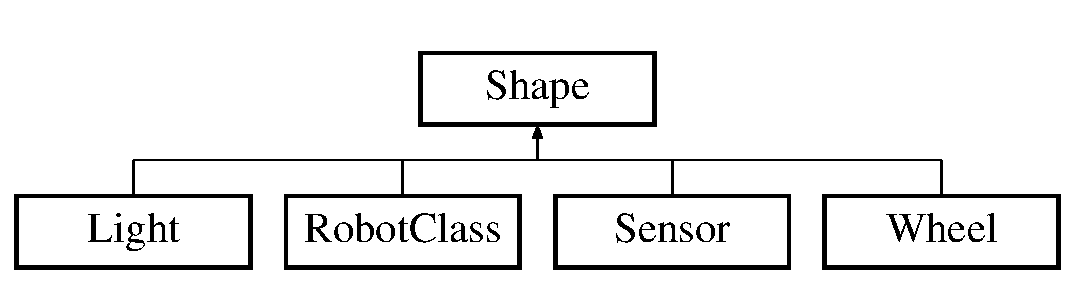
\includegraphics[height=2.000000cm]{classShape}
\end{center}
\end{figure}
\subsection*{Public Member Functions}
\begin{DoxyCompactItemize}
\item 
\hyperlink{classShape_aaa8d87171e65e0d8ba3c5459978992a7}{Shape} ()
\begin{DoxyCompactList}\small\item\em The default constructor. \end{DoxyCompactList}\item 
\hyperlink{classShape_a0321daab69934d93bdbfa0043aa93d6f}{Shape} (double x, double y, double w, double l, double sp, double ori, \hyperlink{Shape_8h_a5a4538eeab397888d88a4eefcc5a1345}{Shape\-Type} st, float c\mbox{[}3\mbox{]})
\begin{DoxyCompactList}\small\item\em A Constructor. \end{DoxyCompactList}\item 
\hyperlink{classShape_a935afc9e576015f967d90de56977167d}{$\sim$\-Shape} ()
\begin{DoxyCompactList}\small\item\em The default deconstructor. \end{DoxyCompactList}\item 
virtual void \hyperlink{classShape_a341d3d37dc6612007affe1b397b689a7}{set\-Position} (double x, double y)
\begin{DoxyCompactList}\small\item\em Set \hyperlink{classShape}{Shape}'s Position through arguements. \end{DoxyCompactList}\item 
void \hyperlink{classShape_a3cff2a1f2501873af1c777bf120b9c9a}{set\-Width} (double w)
\begin{DoxyCompactList}\small\item\em set \hyperlink{classShape}{Shape}'s width through arguement. \end{DoxyCompactList}\item 
void \hyperlink{classShape_ae6391c6b6ed068c3f5a30ed15ffd5903}{set\-Length} (double l)
\begin{DoxyCompactList}\small\item\em set \hyperlink{classShape}{Shape}'s length through arguement. \end{DoxyCompactList}\item 
virtual void \hyperlink{classShape_a23976c8158461838dcbba68b118c9580}{set\-Speed} (double pps)
\begin{DoxyCompactList}\small\item\em set object's speed through arguement. \end{DoxyCompactList}\item 
void \hyperlink{classShape_a51e0ae3cdae9992986711bf9e4de5821}{set\-Orientation} (double degrees)
\begin{DoxyCompactList}\small\item\em Set \hyperlink{classShape}{Shape}'s orientation through arguement. \end{DoxyCompactList}\item 
void \hyperlink{classShape_a610d97f732d655186a3cafa63b6f19fb}{set\-Shape} (\hyperlink{Shape_8h_a5a4538eeab397888d88a4eefcc5a1345}{Shape\-Type} shape)
\begin{DoxyCompactList}\small\item\em Set S\-Hape's shape through arguements. \end{DoxyCompactList}\item 
void \hyperlink{classShape_ae2f26cc38bb9b4018de216f63bf33f03}{set\-Color} (float c\mbox{[}$\,$\mbox{]})
\begin{DoxyCompactList}\small\item\em Set \hyperlink{classShape}{Shape}'s color through arguements. \end{DoxyCompactList}\item 
double \hyperlink{classShape_aa318a705f1462eec42c72a1581175cea}{get\-X\-Position} ()
\begin{DoxyCompactList}\small\item\em Return current x position of \hyperlink{classShape}{Shape}. \end{DoxyCompactList}\item 
double \hyperlink{classShape_a4abaab3fb5f7dd9ec5d370077c8a460d}{get\-Y\-Position} ()
\begin{DoxyCompactList}\small\item\em Return current y position of \hyperlink{classShape}{Shape}. \end{DoxyCompactList}\item 
double \hyperlink{classShape_a512f68cc25140a761d0daaca7e49dc42}{get\-Width} ()
\begin{DoxyCompactList}\small\item\em Return current width of \hyperlink{classShape}{Shape}. \end{DoxyCompactList}\item 
double \hyperlink{classShape_a89fea1a4257a592f4a94626df49af6be}{get\-Length} ()
\begin{DoxyCompactList}\small\item\em Return current length of \hyperlink{classShape}{Shape}. \end{DoxyCompactList}\item 
double \hyperlink{classShape_a5d515965a741032ee2d9ffad45d99f88}{get\-Speed} ()
\begin{DoxyCompactList}\small\item\em Return current speed of object. \end{DoxyCompactList}\item 
double \hyperlink{classShape_a0b50a459fa51ff3ae311fc09194966e6}{get\-Orientation} ()
\begin{DoxyCompactList}\small\item\em Return current orientation of object. \end{DoxyCompactList}\item 
\hyperlink{Shape_8h_a5a4538eeab397888d88a4eefcc5a1345}{Shape\-Type} \hyperlink{classShape_a2ac50956512eba17938466857ba8a069}{get\-Shape\-Type} ()
\begin{DoxyCompactList}\small\item\em Return Object's shape through arguements. \end{DoxyCompactList}\item 
float $\ast$ \hyperlink{classShape_ab27ec7349bf8707b5f1ff4031af0923e}{get\-Color} ()
\begin{DoxyCompactList}\small\item\em Get Object's color through arguements. \end{DoxyCompactList}\item 
double \hyperlink{classShape_a716868f38999597e67b1d1ceaf4e0876}{regular\-\_\-\-Ori} (double d)
\begin{DoxyCompactList}\small\item\em Regulate input degree to make it range from 0 -\/ 360. \end{DoxyCompactList}\end{DoxyCompactItemize}
\subsection*{Private Attributes}
\begin{DoxyCompactItemize}
\item 
\hyperlink{Shape_8h_a5a4538eeab397888d88a4eefcc5a1345}{Shape\-Type} \hyperlink{classShape_a18af04fdf7a9e121518f3c7278693c60}{shape\-Type}
\item 
int \hyperlink{classShape_a24a25c3d22ee7e05d0439f765f247125}{I\-D}
\item 
double \hyperlink{classShape_a018c8854f87fe06796659eb96bf588bc}{width}
\item 
double \hyperlink{classShape_ac63ea3d2c8a8ad0481ec5f6cb9b5dbfc}{length}
\item 
double \hyperlink{classShape_ae07fa065912725b9382c9b58dcaa3a2c}{pos\-\_\-x}
\item 
double \hyperlink{classShape_aa7c6ae5806f6fba2a108e9e04fa98545}{pos\-\_\-y}
\item 
double \hyperlink{classShape_ad426ffc5fe63007bf8dedce3881725a6}{speed}
\item 
double \hyperlink{classShape_a0bbdd420c8befa0a9c5fc95954205e9d}{orientation}
\item 
float \hyperlink{classShape_a9f925188936af909e796807fc75c1501}{color} \mbox{[}3\mbox{]}
\end{DoxyCompactItemize}


\subsection{Detailed Description}
Super Class of \hyperlink{classRobotClass}{Robot\-Class}, Target and Obstacle, contains position x, y, width and length. 

\subsection{Constructor \& Destructor Documentation}
\hypertarget{classShape_aaa8d87171e65e0d8ba3c5459978992a7}{\index{Shape@{Shape}!Shape@{Shape}}
\index{Shape@{Shape}!Shape@{Shape}}
\subsubsection[{Shape}]{\setlength{\rightskip}{0pt plus 5cm}Shape\-::\-Shape (
\begin{DoxyParamCaption}
{}
\end{DoxyParamCaption}
)}}\label{classShape_aaa8d87171e65e0d8ba3c5459978992a7}


The default constructor. 

\begin{DoxyAuthor}{Author}
Zixiao Wang 
\end{DoxyAuthor}
\hypertarget{classShape_a0321daab69934d93bdbfa0043aa93d6f}{\index{Shape@{Shape}!Shape@{Shape}}
\index{Shape@{Shape}!Shape@{Shape}}
\subsubsection[{Shape}]{\setlength{\rightskip}{0pt plus 5cm}Shape\-::\-Shape (
\begin{DoxyParamCaption}
\item[{double}]{x, }
\item[{double}]{y, }
\item[{double}]{w, }
\item[{double}]{l, }
\item[{double}]{sp, }
\item[{double}]{ori, }
\item[{{\bf Shape\-Type}}]{st, }
\item[{float}]{c\mbox{[}3\mbox{]}}
\end{DoxyParamCaption}
)}}\label{classShape_a0321daab69934d93bdbfa0043aa93d6f}


A Constructor. 

\begin{DoxyAuthor}{Author}
Zixiao Wang 
\end{DoxyAuthor}

\begin{DoxyParams}{Parameters}
{\em x} & The x position of \hyperlink{classShape}{Shape}. \\
\hline
{\em y} & The y position of \hyperlink{classShape}{Shape}. \\
\hline
{\em w} & The width of \hyperlink{classShape}{Shape}. \\
\hline
{\em l} & The length of \hyperlink{classShape}{Shape}. \\
\hline
{\em sp} & The speed of \hyperlink{classShape}{Shape}. \\
\hline
{\em ori} & The orientation of \hyperlink{classShape}{Shape}. \\
\hline
{\em st} & The Shape\-Type of \hyperlink{classShape}{Shape}. \\
\hline
{\em c} & The color of \hyperlink{classShape}{Shape}. \\
\hline
\end{DoxyParams}
\hypertarget{classShape_a935afc9e576015f967d90de56977167d}{\index{Shape@{Shape}!$\sim$\-Shape@{$\sim$\-Shape}}
\index{$\sim$\-Shape@{$\sim$\-Shape}!Shape@{Shape}}
\subsubsection[{$\sim$\-Shape}]{\setlength{\rightskip}{0pt plus 5cm}Shape\-::$\sim$\-Shape (
\begin{DoxyParamCaption}
{}
\end{DoxyParamCaption}
)}}\label{classShape_a935afc9e576015f967d90de56977167d}


The default deconstructor. 

\begin{DoxyAuthor}{Author}
Zixiao Wang 
\end{DoxyAuthor}


\subsection{Member Function Documentation}
\hypertarget{classShape_ab27ec7349bf8707b5f1ff4031af0923e}{\index{Shape@{Shape}!get\-Color@{get\-Color}}
\index{get\-Color@{get\-Color}!Shape@{Shape}}
\subsubsection[{get\-Color}]{\setlength{\rightskip}{0pt plus 5cm}float $\ast$ Shape\-::get\-Color (
\begin{DoxyParamCaption}
{}
\end{DoxyParamCaption}
)}}\label{classShape_ab27ec7349bf8707b5f1ff4031af0923e}


Get Object's color through arguements. 

\begin{DoxyAuthor}{Author}
Zixiao Wang 
\end{DoxyAuthor}
\hypertarget{classShape_a89fea1a4257a592f4a94626df49af6be}{\index{Shape@{Shape}!get\-Length@{get\-Length}}
\index{get\-Length@{get\-Length}!Shape@{Shape}}
\subsubsection[{get\-Length}]{\setlength{\rightskip}{0pt plus 5cm}double Shape\-::get\-Length (
\begin{DoxyParamCaption}
{}
\end{DoxyParamCaption}
)}}\label{classShape_a89fea1a4257a592f4a94626df49af6be}


Return current length of \hyperlink{classShape}{Shape}. 

\begin{DoxyAuthor}{Author}
Zixiao Wang 
\end{DoxyAuthor}
\hypertarget{classShape_a0b50a459fa51ff3ae311fc09194966e6}{\index{Shape@{Shape}!get\-Orientation@{get\-Orientation}}
\index{get\-Orientation@{get\-Orientation}!Shape@{Shape}}
\subsubsection[{get\-Orientation}]{\setlength{\rightskip}{0pt plus 5cm}double Shape\-::get\-Orientation (
\begin{DoxyParamCaption}
{}
\end{DoxyParamCaption}
)}}\label{classShape_a0b50a459fa51ff3ae311fc09194966e6}


Return current orientation of object. 

\begin{DoxyAuthor}{Author}
Zixiao Wang 
\end{DoxyAuthor}
\hypertarget{classShape_a2ac50956512eba17938466857ba8a069}{\index{Shape@{Shape}!get\-Shape\-Type@{get\-Shape\-Type}}
\index{get\-Shape\-Type@{get\-Shape\-Type}!Shape@{Shape}}
\subsubsection[{get\-Shape\-Type}]{\setlength{\rightskip}{0pt plus 5cm}{\bf Shape\-Type} Shape\-::get\-Shape\-Type (
\begin{DoxyParamCaption}
{}
\end{DoxyParamCaption}
)}}\label{classShape_a2ac50956512eba17938466857ba8a069}


Return Object's shape through arguements. 

\begin{DoxyAuthor}{Author}
Zixiao Wang 
\end{DoxyAuthor}
\hypertarget{classShape_a5d515965a741032ee2d9ffad45d99f88}{\index{Shape@{Shape}!get\-Speed@{get\-Speed}}
\index{get\-Speed@{get\-Speed}!Shape@{Shape}}
\subsubsection[{get\-Speed}]{\setlength{\rightskip}{0pt plus 5cm}double Shape\-::get\-Speed (
\begin{DoxyParamCaption}
{}
\end{DoxyParamCaption}
)}}\label{classShape_a5d515965a741032ee2d9ffad45d99f88}


Return current speed of object. 

\begin{DoxyAuthor}{Author}
Zixiao Wang 
\end{DoxyAuthor}
\hypertarget{classShape_a512f68cc25140a761d0daaca7e49dc42}{\index{Shape@{Shape}!get\-Width@{get\-Width}}
\index{get\-Width@{get\-Width}!Shape@{Shape}}
\subsubsection[{get\-Width}]{\setlength{\rightskip}{0pt plus 5cm}double Shape\-::get\-Width (
\begin{DoxyParamCaption}
{}
\end{DoxyParamCaption}
)}}\label{classShape_a512f68cc25140a761d0daaca7e49dc42}


Return current width of \hyperlink{classShape}{Shape}. 

\begin{DoxyAuthor}{Author}
Zixiao Wang 
\end{DoxyAuthor}
\hypertarget{classShape_aa318a705f1462eec42c72a1581175cea}{\index{Shape@{Shape}!get\-X\-Position@{get\-X\-Position}}
\index{get\-X\-Position@{get\-X\-Position}!Shape@{Shape}}
\subsubsection[{get\-X\-Position}]{\setlength{\rightskip}{0pt plus 5cm}double Shape\-::get\-X\-Position (
\begin{DoxyParamCaption}
{}
\end{DoxyParamCaption}
)}}\label{classShape_aa318a705f1462eec42c72a1581175cea}


Return current x position of \hyperlink{classShape}{Shape}. 

\begin{DoxyAuthor}{Author}
Zixiao Wang 
\end{DoxyAuthor}
\hypertarget{classShape_a4abaab3fb5f7dd9ec5d370077c8a460d}{\index{Shape@{Shape}!get\-Y\-Position@{get\-Y\-Position}}
\index{get\-Y\-Position@{get\-Y\-Position}!Shape@{Shape}}
\subsubsection[{get\-Y\-Position}]{\setlength{\rightskip}{0pt plus 5cm}double Shape\-::get\-Y\-Position (
\begin{DoxyParamCaption}
{}
\end{DoxyParamCaption}
)}}\label{classShape_a4abaab3fb5f7dd9ec5d370077c8a460d}


Return current y position of \hyperlink{classShape}{Shape}. 

\begin{DoxyAuthor}{Author}
Zixiao Wang 
\end{DoxyAuthor}
\hypertarget{classShape_a716868f38999597e67b1d1ceaf4e0876}{\index{Shape@{Shape}!regular\-\_\-\-Ori@{regular\-\_\-\-Ori}}
\index{regular\-\_\-\-Ori@{regular\-\_\-\-Ori}!Shape@{Shape}}
\subsubsection[{regular\-\_\-\-Ori}]{\setlength{\rightskip}{0pt plus 5cm}double Shape\-::regular\-\_\-\-Ori (
\begin{DoxyParamCaption}
\item[{double}]{d}
\end{DoxyParamCaption}
)}}\label{classShape_a716868f38999597e67b1d1ceaf4e0876}


Regulate input degree to make it range from 0 -\/ 360. 

\begin{DoxyAuthor}{Author}
Zixiao Wang 
\end{DoxyAuthor}
\hypertarget{classShape_ae2f26cc38bb9b4018de216f63bf33f03}{\index{Shape@{Shape}!set\-Color@{set\-Color}}
\index{set\-Color@{set\-Color}!Shape@{Shape}}
\subsubsection[{set\-Color}]{\setlength{\rightskip}{0pt plus 5cm}void Shape\-::set\-Color (
\begin{DoxyParamCaption}
\item[{float}]{c\mbox{[}$\,$\mbox{]}}
\end{DoxyParamCaption}
)}}\label{classShape_ae2f26cc38bb9b4018de216f63bf33f03}


Set \hyperlink{classShape}{Shape}'s color through arguements. 

\begin{DoxyAuthor}{Author}
Zixiao Wang 
\end{DoxyAuthor}

\begin{DoxyParams}{Parameters}
{\em c\mbox{[}$\,$\mbox{]}} & Set \hyperlink{classShape}{Shape}'s color according to the array passed in. \\
\hline
\end{DoxyParams}
\hypertarget{classShape_ae6391c6b6ed068c3f5a30ed15ffd5903}{\index{Shape@{Shape}!set\-Length@{set\-Length}}
\index{set\-Length@{set\-Length}!Shape@{Shape}}
\subsubsection[{set\-Length}]{\setlength{\rightskip}{0pt plus 5cm}void Shape\-::set\-Length (
\begin{DoxyParamCaption}
\item[{double}]{l}
\end{DoxyParamCaption}
)}}\label{classShape_ae6391c6b6ed068c3f5a30ed15ffd5903}


set \hyperlink{classShape}{Shape}'s length through arguement. 

\begin{DoxyAuthor}{Author}
Zixiao Wang 
\end{DoxyAuthor}

\begin{DoxyParams}{Parameters}
{\em l} & Set \hyperlink{classShape}{Shape}'s length according to arguement double l. \\
\hline
\end{DoxyParams}
\hypertarget{classShape_a51e0ae3cdae9992986711bf9e4de5821}{\index{Shape@{Shape}!set\-Orientation@{set\-Orientation}}
\index{set\-Orientation@{set\-Orientation}!Shape@{Shape}}
\subsubsection[{set\-Orientation}]{\setlength{\rightskip}{0pt plus 5cm}void Shape\-::set\-Orientation (
\begin{DoxyParamCaption}
\item[{double}]{degrees}
\end{DoxyParamCaption}
)}}\label{classShape_a51e0ae3cdae9992986711bf9e4de5821}


Set \hyperlink{classShape}{Shape}'s orientation through arguement. 

\begin{DoxyAuthor}{Author}
Zixiao Wang 
\end{DoxyAuthor}

\begin{DoxyParams}{Parameters}
{\em degrees} & Set \hyperlink{classShape}{Shape}'s orientation according to arguement integer degrees. \\
\hline
\end{DoxyParams}
\hypertarget{classShape_a341d3d37dc6612007affe1b397b689a7}{\index{Shape@{Shape}!set\-Position@{set\-Position}}
\index{set\-Position@{set\-Position}!Shape@{Shape}}
\subsubsection[{set\-Position}]{\setlength{\rightskip}{0pt plus 5cm}void Shape\-::set\-Position (
\begin{DoxyParamCaption}
\item[{double}]{x, }
\item[{double}]{y}
\end{DoxyParamCaption}
)\hspace{0.3cm}{\ttfamily [virtual]}}}\label{classShape_a341d3d37dc6612007affe1b397b689a7}


Set \hyperlink{classShape}{Shape}'s Position through arguements. 

\begin{DoxyAuthor}{Author}
Zixiao Wang 
\end{DoxyAuthor}

\begin{DoxyParams}{Parameters}
{\em x} & Set \hyperlink{classShape}{Shape}'s position according to arguement double x. \\
\hline
{\em y} & Set \hyperlink{classShape}{Shape}'s position according to arguement double y. \\
\hline
\end{DoxyParams}
\hypertarget{classShape_a610d97f732d655186a3cafa63b6f19fb}{\index{Shape@{Shape}!set\-Shape@{set\-Shape}}
\index{set\-Shape@{set\-Shape}!Shape@{Shape}}
\subsubsection[{set\-Shape}]{\setlength{\rightskip}{0pt plus 5cm}void Shape\-::set\-Shape (
\begin{DoxyParamCaption}
\item[{{\bf Shape\-Type}}]{shape}
\end{DoxyParamCaption}
)}}\label{classShape_a610d97f732d655186a3cafa63b6f19fb}


Set S\-Hape's shape through arguements. 

\begin{DoxyAuthor}{Author}
Zixiao Wang 
\end{DoxyAuthor}

\begin{DoxyParams}{Parameters}
{\em shape} & Set \hyperlink{classShape}{Shape}'s shape according to the shape passed in. \\
\hline
\end{DoxyParams}
\hypertarget{classShape_a23976c8158461838dcbba68b118c9580}{\index{Shape@{Shape}!set\-Speed@{set\-Speed}}
\index{set\-Speed@{set\-Speed}!Shape@{Shape}}
\subsubsection[{set\-Speed}]{\setlength{\rightskip}{0pt plus 5cm}void Shape\-::set\-Speed (
\begin{DoxyParamCaption}
\item[{double}]{pps}
\end{DoxyParamCaption}
)\hspace{0.3cm}{\ttfamily [virtual]}}}\label{classShape_a23976c8158461838dcbba68b118c9580}


set object's speed through arguement. 

\begin{DoxyAuthor}{Author}
Zixiao Wang 
\end{DoxyAuthor}

\begin{DoxyParams}{Parameters}
{\em pps} & Set object's speed according to arguement integer pps. \\
\hline
\end{DoxyParams}
\hypertarget{classShape_a3cff2a1f2501873af1c777bf120b9c9a}{\index{Shape@{Shape}!set\-Width@{set\-Width}}
\index{set\-Width@{set\-Width}!Shape@{Shape}}
\subsubsection[{set\-Width}]{\setlength{\rightskip}{0pt plus 5cm}void Shape\-::set\-Width (
\begin{DoxyParamCaption}
\item[{double}]{w}
\end{DoxyParamCaption}
)}}\label{classShape_a3cff2a1f2501873af1c777bf120b9c9a}


set \hyperlink{classShape}{Shape}'s width through arguement. 

\begin{DoxyAuthor}{Author}
Zixiao Wang 
\end{DoxyAuthor}

\begin{DoxyParams}{Parameters}
{\em w} & Set \hyperlink{classShape}{Shape}'s width according to arguement double w. \\
\hline
\end{DoxyParams}


\subsection{Member Data Documentation}
\hypertarget{classShape_a9f925188936af909e796807fc75c1501}{\index{Shape@{Shape}!color@{color}}
\index{color@{color}!Shape@{Shape}}
\subsubsection[{color}]{\setlength{\rightskip}{0pt plus 5cm}float Shape\-::color\mbox{[}3\mbox{]}\hspace{0.3cm}{\ttfamily [private]}}}\label{classShape_a9f925188936af909e796807fc75c1501}
color of shape \hypertarget{classShape_a24a25c3d22ee7e05d0439f765f247125}{\index{Shape@{Shape}!I\-D@{I\-D}}
\index{I\-D@{I\-D}!Shape@{Shape}}
\subsubsection[{I\-D}]{\setlength{\rightskip}{0pt plus 5cm}int Shape\-::\-I\-D\hspace{0.3cm}{\ttfamily [private]}}}\label{classShape_a24a25c3d22ee7e05d0439f765f247125}
\hypertarget{classShape_ac63ea3d2c8a8ad0481ec5f6cb9b5dbfc}{\index{Shape@{Shape}!length@{length}}
\index{length@{length}!Shape@{Shape}}
\subsubsection[{length}]{\setlength{\rightskip}{0pt plus 5cm}double Shape\-::length\hspace{0.3cm}{\ttfamily [private]}}}\label{classShape_ac63ea3d2c8a8ad0481ec5f6cb9b5dbfc}
length of shape \hypertarget{classShape_a0bbdd420c8befa0a9c5fc95954205e9d}{\index{Shape@{Shape}!orientation@{orientation}}
\index{orientation@{orientation}!Shape@{Shape}}
\subsubsection[{orientation}]{\setlength{\rightskip}{0pt plus 5cm}double Shape\-::orientation\hspace{0.3cm}{\ttfamily [private]}}}\label{classShape_a0bbdd420c8befa0a9c5fc95954205e9d}
direction of shape \hypertarget{classShape_ae07fa065912725b9382c9b58dcaa3a2c}{\index{Shape@{Shape}!pos\-\_\-x@{pos\-\_\-x}}
\index{pos\-\_\-x@{pos\-\_\-x}!Shape@{Shape}}
\subsubsection[{pos\-\_\-x}]{\setlength{\rightskip}{0pt plus 5cm}double Shape\-::pos\-\_\-x\hspace{0.3cm}{\ttfamily [private]}}}\label{classShape_ae07fa065912725b9382c9b58dcaa3a2c}
x position of shape \hypertarget{classShape_aa7c6ae5806f6fba2a108e9e04fa98545}{\index{Shape@{Shape}!pos\-\_\-y@{pos\-\_\-y}}
\index{pos\-\_\-y@{pos\-\_\-y}!Shape@{Shape}}
\subsubsection[{pos\-\_\-y}]{\setlength{\rightskip}{0pt plus 5cm}double Shape\-::pos\-\_\-y\hspace{0.3cm}{\ttfamily [private]}}}\label{classShape_aa7c6ae5806f6fba2a108e9e04fa98545}
y position of shape \hypertarget{classShape_a18af04fdf7a9e121518f3c7278693c60}{\index{Shape@{Shape}!shape\-Type@{shape\-Type}}
\index{shape\-Type@{shape\-Type}!Shape@{Shape}}
\subsubsection[{shape\-Type}]{\setlength{\rightskip}{0pt plus 5cm}{\bf Shape\-Type} Shape\-::shape\-Type\hspace{0.3cm}{\ttfamily [private]}}}\label{classShape_a18af04fdf7a9e121518f3c7278693c60}
\hypertarget{classShape_ad426ffc5fe63007bf8dedce3881725a6}{\index{Shape@{Shape}!speed@{speed}}
\index{speed@{speed}!Shape@{Shape}}
\subsubsection[{speed}]{\setlength{\rightskip}{0pt plus 5cm}double Shape\-::speed\hspace{0.3cm}{\ttfamily [private]}}}\label{classShape_ad426ffc5fe63007bf8dedce3881725a6}
speed of shape \hypertarget{classShape_a018c8854f87fe06796659eb96bf588bc}{\index{Shape@{Shape}!width@{width}}
\index{width@{width}!Shape@{Shape}}
\subsubsection[{width}]{\setlength{\rightskip}{0pt plus 5cm}double Shape\-::width\hspace{0.3cm}{\ttfamily [private]}}}\label{classShape_a018c8854f87fe06796659eb96bf588bc}
width of shape 

The documentation for this class was generated from the following files\-:\begin{DoxyCompactItemize}
\item 
\hyperlink{Shape_8h}{Shape.\-h}\item 
\hyperlink{Shape_8cpp}{Shape.\-cpp}\end{DoxyCompactItemize}

\hypertarget{classSimulation}{\section{Simulation Class Reference}
\label{classSimulation}\index{Simulation@{Simulation}}
}


{\ttfamily \#include $<$Simulation.\-h$>$}

Inheritance diagram for Simulation\-:\begin{figure}[H]
\begin{center}
\leavevmode
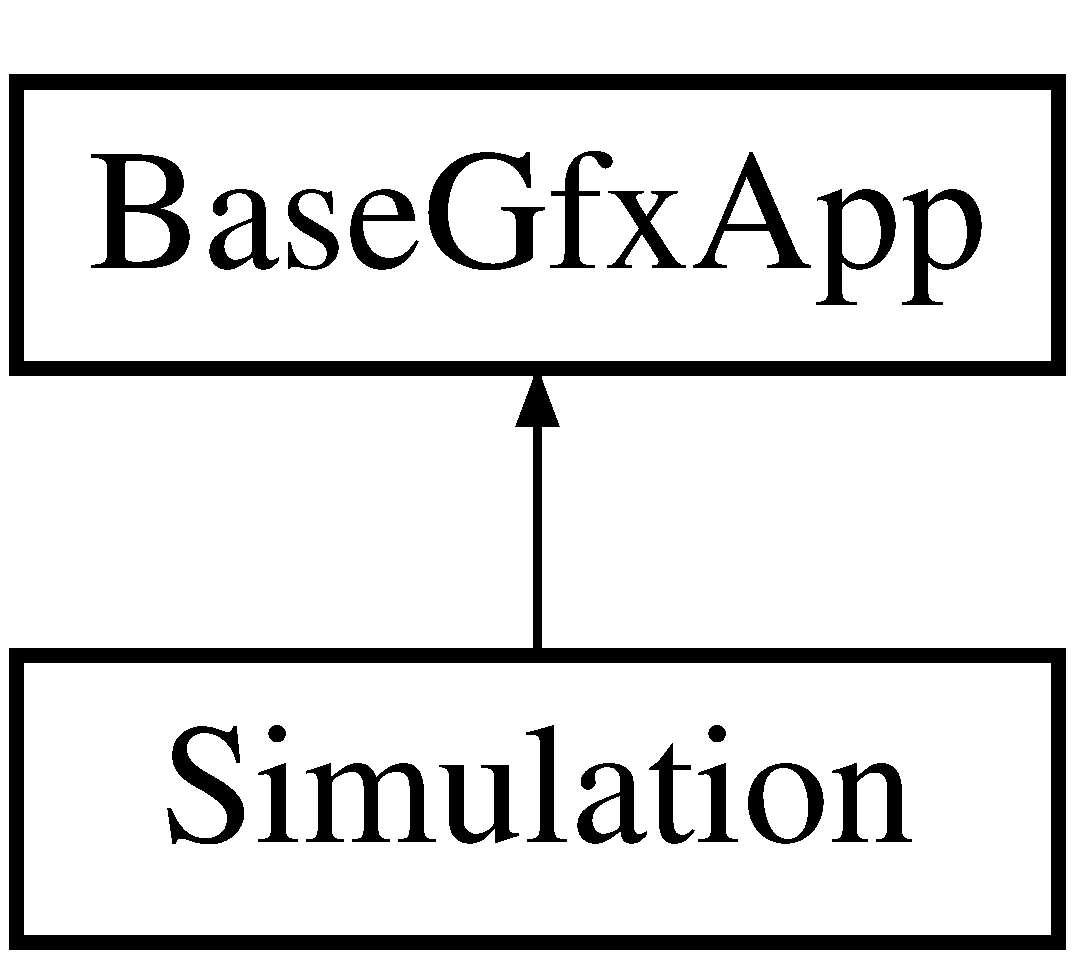
\includegraphics[height=2.000000cm]{classSimulation}
\end{center}
\end{figure}
\subsection*{Public Types}
\begin{DoxyCompactItemize}
\item 
enum \hyperlink{classSimulation_a0fd1c91d4e7699e893929d56b60a60bf}{U\-I\-Control\-Type} \{ \\*
\hyperlink{classSimulation_a0fd1c91d4e7699e893929d56b60a60bfa51f628c4a96a151830bd4a541dc42a5f}{U\-I\-\_\-\-Q\-U\-I\-T}, 
\hyperlink{classSimulation_a0fd1c91d4e7699e893929d56b60a60bfae8829fdccf0a3a28e0b0bf8dc47bf26e}{U\-I\-\_\-\-R\-E\-S\-U\-M\-E}, 
\hyperlink{classSimulation_a0fd1c91d4e7699e893929d56b60a60bfa6eb81d656b8ff64239548e4195560ef0}{U\-I\-\_\-\-P\-A\-U\-S\-E}, 
\hyperlink{classSimulation_a0fd1c91d4e7699e893929d56b60a60bfae4ec551adee29b6e2329929952c10ce5}{U\-I\-\_\-\-S\-T\-A\-R\-T}, 
\\*
\hyperlink{classSimulation_a0fd1c91d4e7699e893929d56b60a60bfa34512906ee0d0aafcd7f3257f738de15}{U\-I\-\_\-\-S\-P\-I\-N}
 \}
\begin{DoxyCompactList}\small\item\em the type of U\-I Control input. \end{DoxyCompactList}\end{DoxyCompactItemize}
\subsection*{Public Member Functions}
\begin{DoxyCompactItemize}
\item 
\hyperlink{classSimulation_a4c669ceaa34c7130966ce45f9de75fbe}{Simulation} (int argc, char $\ast$argv\mbox{[}$\,$\mbox{]}, int \hyperlink{classBaseGfxApp_ace089a1a94fb6bb0bc17e1b7fa48e05d}{width}, int \hyperlink{classBaseGfxApp_aa253dbe16a20c40e0a1bf8ff942ceea3}{height})
\begin{DoxyCompactList}\small\item\em arguements from user's command input and other window information. \end{DoxyCompactList}\item 
virtual \hyperlink{classSimulation_a80fad3f57dfaf195a36f7bc49bc88279}{$\sim$\-Simulation} ()
\item 
void \hyperlink{classSimulation_a449dcb7d97dfba99efe770de2f399c31}{display} ()
\begin{DoxyCompactList}\small\item\em display all the items. \end{DoxyCompactList}\item 
void \hyperlink{classSimulation_a1607cd18e552ab9f4a6f57d362f7121a}{glui\-Control} (int control\-I\-D)
\begin{DoxyCompactList}\small\item\em set controlflag value, in order to implement control panel. \end{DoxyCompactList}\item 
void \hyperlink{classSimulation_aa975d7962f1ea62a2c3a1ae42392d906}{render\-Robot} (\hyperlink{classRobotClass}{Robot\-Class} robot, int \hyperlink{classSimulation_a5a5e26d75c6a6dee8cdfecc7669545e3}{count})
\begin{DoxyCompactList}\small\item\em draw robot and send it to the window. \end{DoxyCompactList}\item 
void \hyperlink{classSimulation_a43ebad86548efc30eb3a3e9959002aaa}{render\-Light} (\hyperlink{classLight}{Light} light, int \hyperlink{classSimulation_a5a5e26d75c6a6dee8cdfecc7669545e3}{count})
\begin{DoxyCompactList}\small\item\em draw light and send it to the window. \end{DoxyCompactList}\item 
void \hyperlink{classSimulation_a786d1ba31d29937f0ac6f3ea88f8a607}{left\-Mouse\-Down} (int x, int y)
\begin{DoxyCompactList}\small\item\em The action will be taken when left mouse is clicked. \end{DoxyCompactList}\item 
void \hyperlink{classSimulation_a62ef254d85017074cd521a5787b5a234}{left\-Mouse\-Up} (int x, int y)
\begin{DoxyCompactList}\small\item\em The action will be taken when right mouse is clicked. \end{DoxyCompactList}\end{DoxyCompactItemize}
\subsection*{Private Attributes}
\begin{DoxyCompactItemize}
\item 
bool \hyperlink{classSimulation_a99785aef857b01f3056bada702b53d20}{controlflag}
\item 
int \hyperlink{classSimulation_aed3fe9fceae4a68746206b7a2f9e9d7f}{num\-Robot}
\item 
int \hyperlink{classSimulation_a792ef5172ff14046a641661ce2a95041}{num\-Light}
\item 
double \hyperlink{classSimulation_a9d5a2c76548907940c15b389344365df}{old\-Time\-Since\-Start}
\item 
vector$<$ \hyperlink{classRobotClass}{Robot\-Class} $>$ \hyperlink{classSimulation_ac48312060cc6b3b973bba8c802b45bce}{robots}
\item 
vector$<$ \hyperlink{classLight}{Light} $>$ \hyperlink{classSimulation_a4f6efa5f1bb16876c98f134fe80e9278}{lights}
\item 
\hyperlink{classEnvironmentClass}{Environment\-Class} $\ast$ \hyperlink{classSimulation_adb82ccf6c2a4b78c73987857f5362a35}{env}
\item 
G\-L\-U\-I\-\_\-\-Spinner $\ast$ \hyperlink{classSimulation_ade4b147d7d59002d1ea81b60bba84b48}{spinner}
\item 
int \hyperlink{classSimulation_a5a5e26d75c6a6dee8cdfecc7669545e3}{count}
\end{DoxyCompactItemize}
\subsection*{Additional Inherited Members}


\subsection{Detailed Description}
The \hyperlink{classSimulation}{Simulation} class. This sets up the G\-U\-I and the drawing environment. 

\subsection{Member Enumeration Documentation}
\hypertarget{classSimulation_a0fd1c91d4e7699e893929d56b60a60bf}{\index{Simulation@{Simulation}!U\-I\-Control\-Type@{U\-I\-Control\-Type}}
\index{U\-I\-Control\-Type@{U\-I\-Control\-Type}!Simulation@{Simulation}}
\subsubsection[{U\-I\-Control\-Type}]{\setlength{\rightskip}{0pt plus 5cm}enum {\bf Simulation\-::\-U\-I\-Control\-Type}}}\label{classSimulation_a0fd1c91d4e7699e893929d56b60a60bf}


the type of U\-I Control input. 

\begin{DoxyAuthor}{Author}
Zixiao Wang 
\end{DoxyAuthor}
\begin{Desc}
\item[Enumerator]\par
\begin{description}
\index{U\-I\-\_\-\-Q\-U\-I\-T@{U\-I\-\_\-\-Q\-U\-I\-T}!Simulation@{Simulation}}\index{Simulation@{Simulation}!U\-I\-\_\-\-Q\-U\-I\-T@{U\-I\-\_\-\-Q\-U\-I\-T}}\item[{\em 
\hypertarget{classSimulation_a0fd1c91d4e7699e893929d56b60a60bfa51f628c4a96a151830bd4a541dc42a5f}{U\-I\-\_\-\-Q\-U\-I\-T}\label{classSimulation_a0fd1c91d4e7699e893929d56b60a60bfa51f628c4a96a151830bd4a541dc42a5f}
}]\index{U\-I\-\_\-\-R\-E\-S\-U\-M\-E@{U\-I\-\_\-\-R\-E\-S\-U\-M\-E}!Simulation@{Simulation}}\index{Simulation@{Simulation}!U\-I\-\_\-\-R\-E\-S\-U\-M\-E@{U\-I\-\_\-\-R\-E\-S\-U\-M\-E}}\item[{\em 
\hypertarget{classSimulation_a0fd1c91d4e7699e893929d56b60a60bfae8829fdccf0a3a28e0b0bf8dc47bf26e}{U\-I\-\_\-\-R\-E\-S\-U\-M\-E}\label{classSimulation_a0fd1c91d4e7699e893929d56b60a60bfae8829fdccf0a3a28e0b0bf8dc47bf26e}
}]\index{U\-I\-\_\-\-P\-A\-U\-S\-E@{U\-I\-\_\-\-P\-A\-U\-S\-E}!Simulation@{Simulation}}\index{Simulation@{Simulation}!U\-I\-\_\-\-P\-A\-U\-S\-E@{U\-I\-\_\-\-P\-A\-U\-S\-E}}\item[{\em 
\hypertarget{classSimulation_a0fd1c91d4e7699e893929d56b60a60bfa6eb81d656b8ff64239548e4195560ef0}{U\-I\-\_\-\-P\-A\-U\-S\-E}\label{classSimulation_a0fd1c91d4e7699e893929d56b60a60bfa6eb81d656b8ff64239548e4195560ef0}
}]\index{U\-I\-\_\-\-S\-T\-A\-R\-T@{U\-I\-\_\-\-S\-T\-A\-R\-T}!Simulation@{Simulation}}\index{Simulation@{Simulation}!U\-I\-\_\-\-S\-T\-A\-R\-T@{U\-I\-\_\-\-S\-T\-A\-R\-T}}\item[{\em 
\hypertarget{classSimulation_a0fd1c91d4e7699e893929d56b60a60bfae4ec551adee29b6e2329929952c10ce5}{U\-I\-\_\-\-S\-T\-A\-R\-T}\label{classSimulation_a0fd1c91d4e7699e893929d56b60a60bfae4ec551adee29b6e2329929952c10ce5}
}]\index{U\-I\-\_\-\-S\-P\-I\-N@{U\-I\-\_\-\-S\-P\-I\-N}!Simulation@{Simulation}}\index{Simulation@{Simulation}!U\-I\-\_\-\-S\-P\-I\-N@{U\-I\-\_\-\-S\-P\-I\-N}}\item[{\em 
\hypertarget{classSimulation_a0fd1c91d4e7699e893929d56b60a60bfa34512906ee0d0aafcd7f3257f738de15}{U\-I\-\_\-\-S\-P\-I\-N}\label{classSimulation_a0fd1c91d4e7699e893929d56b60a60bfa34512906ee0d0aafcd7f3257f738de15}
}]\end{description}
\end{Desc}


\subsection{Constructor \& Destructor Documentation}
\hypertarget{classSimulation_a4c669ceaa34c7130966ce45f9de75fbe}{\index{Simulation@{Simulation}!Simulation@{Simulation}}
\index{Simulation@{Simulation}!Simulation@{Simulation}}
\subsubsection[{Simulation}]{\setlength{\rightskip}{0pt plus 5cm}Simulation\-::\-Simulation (
\begin{DoxyParamCaption}
\item[{int}]{argc, }
\item[{char $\ast$}]{argv\mbox{[}$\,$\mbox{]}, }
\item[{int}]{width, }
\item[{int}]{height}
\end{DoxyParamCaption}
)}}\label{classSimulation_a4c669ceaa34c7130966ce45f9de75fbe}


arguements from user's command input and other window information. 

\begin{DoxyAuthor}{Author}
Zixiao Wang 
\end{DoxyAuthor}

\begin{DoxyParams}{Parameters}
{\em argc} & The number of command arguement. \\
\hline
{\em argv} & The command input array. \\
\hline
{\em width} & The width of window. \\
\hline
{\em height} & The height of window. \\
\hline
\end{DoxyParams}
\hypertarget{classSimulation_a80fad3f57dfaf195a36f7bc49bc88279}{\index{Simulation@{Simulation}!$\sim$\-Simulation@{$\sim$\-Simulation}}
\index{$\sim$\-Simulation@{$\sim$\-Simulation}!Simulation@{Simulation}}
\subsubsection[{$\sim$\-Simulation}]{\setlength{\rightskip}{0pt plus 5cm}Simulation\-::$\sim$\-Simulation (
\begin{DoxyParamCaption}
{}
\end{DoxyParamCaption}
)\hspace{0.3cm}{\ttfamily [virtual]}}}\label{classSimulation_a80fad3f57dfaf195a36f7bc49bc88279}


\subsection{Member Function Documentation}
\hypertarget{classSimulation_a449dcb7d97dfba99efe770de2f399c31}{\index{Simulation@{Simulation}!display@{display}}
\index{display@{display}!Simulation@{Simulation}}
\subsubsection[{display}]{\setlength{\rightskip}{0pt plus 5cm}void Simulation\-::display (
\begin{DoxyParamCaption}
{}
\end{DoxyParamCaption}
)\hspace{0.3cm}{\ttfamily [virtual]}}}\label{classSimulation_a449dcb7d97dfba99efe770de2f399c31}


display all the items. 

\begin{DoxyAuthor}{Author}
Zixiao Wang and Triny Chen 
\end{DoxyAuthor}


Reimplemented from \hyperlink{classBaseGfxApp_ac8de2d5a955582547af5619b771b4d6d}{Base\-Gfx\-App}.

\hypertarget{classSimulation_a1607cd18e552ab9f4a6f57d362f7121a}{\index{Simulation@{Simulation}!glui\-Control@{glui\-Control}}
\index{glui\-Control@{glui\-Control}!Simulation@{Simulation}}
\subsubsection[{glui\-Control}]{\setlength{\rightskip}{0pt plus 5cm}void Simulation\-::glui\-Control (
\begin{DoxyParamCaption}
\item[{int}]{control\-I\-D}
\end{DoxyParamCaption}
)\hspace{0.3cm}{\ttfamily [virtual]}}}\label{classSimulation_a1607cd18e552ab9f4a6f57d362f7121a}


set controlflag value, in order to implement control panel. 

\begin{DoxyAuthor}{Author}
Zixiao Wang 
\end{DoxyAuthor}


Reimplemented from \hyperlink{classBaseGfxApp_a2978a7c358794c67df73b66776b2cef3}{Base\-Gfx\-App}.

\hypertarget{classSimulation_a786d1ba31d29937f0ac6f3ea88f8a607}{\index{Simulation@{Simulation}!left\-Mouse\-Down@{left\-Mouse\-Down}}
\index{left\-Mouse\-Down@{left\-Mouse\-Down}!Simulation@{Simulation}}
\subsubsection[{left\-Mouse\-Down}]{\setlength{\rightskip}{0pt plus 5cm}void Simulation\-::left\-Mouse\-Down (
\begin{DoxyParamCaption}
\item[{int}]{x, }
\item[{int}]{y}
\end{DoxyParamCaption}
)\hspace{0.3cm}{\ttfamily [virtual]}}}\label{classSimulation_a786d1ba31d29937f0ac6f3ea88f8a607}


The action will be taken when left mouse is clicked. 


\begin{DoxyParams}{Parameters}
{\em x} & the x position of mouse click position. \\
\hline
{\em y} & the y position of mouse click position. \\
\hline
\end{DoxyParams}


Reimplemented from \hyperlink{classBaseGfxApp_aaaccf5a5e923a9465441a5ee712424a8}{Base\-Gfx\-App}.

\hypertarget{classSimulation_a62ef254d85017074cd521a5787b5a234}{\index{Simulation@{Simulation}!left\-Mouse\-Up@{left\-Mouse\-Up}}
\index{left\-Mouse\-Up@{left\-Mouse\-Up}!Simulation@{Simulation}}
\subsubsection[{left\-Mouse\-Up}]{\setlength{\rightskip}{0pt plus 5cm}void Simulation\-::left\-Mouse\-Up (
\begin{DoxyParamCaption}
\item[{int}]{x, }
\item[{int}]{y}
\end{DoxyParamCaption}
)\hspace{0.3cm}{\ttfamily [virtual]}}}\label{classSimulation_a62ef254d85017074cd521a5787b5a234}


The action will be taken when right mouse is clicked. 


\begin{DoxyParams}{Parameters}
{\em x} & the x position of mouse click position. \\
\hline
{\em y} & the y position of mouse click position. \\
\hline
\end{DoxyParams}


Reimplemented from \hyperlink{classBaseGfxApp_a0a2961a932b02b2f9d7d0bb408f6fb51}{Base\-Gfx\-App}.

\hypertarget{classSimulation_a43ebad86548efc30eb3a3e9959002aaa}{\index{Simulation@{Simulation}!render\-Light@{render\-Light}}
\index{render\-Light@{render\-Light}!Simulation@{Simulation}}
\subsubsection[{render\-Light}]{\setlength{\rightskip}{0pt plus 5cm}void Simulation\-::render\-Light (
\begin{DoxyParamCaption}
\item[{{\bf Light}}]{light, }
\item[{int}]{count}
\end{DoxyParamCaption}
)}}\label{classSimulation_a43ebad86548efc30eb3a3e9959002aaa}


draw light and send it to the window. 

\begin{DoxyAuthor}{Author}
Zixiao Wang 
\end{DoxyAuthor}

\begin{DoxyParams}{Parameters}
{\em light} & pass in the light which is to be sent. \\
\hline
{\em count} & used for changing color \\
\hline
\end{DoxyParams}
\hypertarget{classSimulation_aa975d7962f1ea62a2c3a1ae42392d906}{\index{Simulation@{Simulation}!render\-Robot@{render\-Robot}}
\index{render\-Robot@{render\-Robot}!Simulation@{Simulation}}
\subsubsection[{render\-Robot}]{\setlength{\rightskip}{0pt plus 5cm}void Simulation\-::render\-Robot (
\begin{DoxyParamCaption}
\item[{{\bf Robot\-Class}}]{robot, }
\item[{int}]{count}
\end{DoxyParamCaption}
)}}\label{classSimulation_aa975d7962f1ea62a2c3a1ae42392d906}


draw robot and send it to the window. 

\begin{DoxyAuthor}{Author}
Zixiao Wang 
\end{DoxyAuthor}

\begin{DoxyParams}{Parameters}
{\em robot} & pass in the robot which is to be sent. \\
\hline
{\em count} & used for changing color \\
\hline
\end{DoxyParams}


\subsection{Member Data Documentation}
\hypertarget{classSimulation_a99785aef857b01f3056bada702b53d20}{\index{Simulation@{Simulation}!controlflag@{controlflag}}
\index{controlflag@{controlflag}!Simulation@{Simulation}}
\subsubsection[{controlflag}]{\setlength{\rightskip}{0pt plus 5cm}bool Simulation\-::controlflag\hspace{0.3cm}{\ttfamily [private]}}}\label{classSimulation_a99785aef857b01f3056bada702b53d20}
The flag for panel input \hypertarget{classSimulation_a5a5e26d75c6a6dee8cdfecc7669545e3}{\index{Simulation@{Simulation}!count@{count}}
\index{count@{count}!Simulation@{Simulation}}
\subsubsection[{count}]{\setlength{\rightskip}{0pt plus 5cm}int Simulation\-::count\hspace{0.3cm}{\ttfamily [private]}}}\label{classSimulation_a5a5e26d75c6a6dee8cdfecc7669545e3}
\hypertarget{classSimulation_adb82ccf6c2a4b78c73987857f5362a35}{\index{Simulation@{Simulation}!env@{env}}
\index{env@{env}!Simulation@{Simulation}}
\subsubsection[{env}]{\setlength{\rightskip}{0pt plus 5cm}{\bf Environment\-Class}$\ast$ Simulation\-::env\hspace{0.3cm}{\ttfamily [private]}}}\label{classSimulation_adb82ccf6c2a4b78c73987857f5362a35}
A environment created \hypertarget{classSimulation_a4f6efa5f1bb16876c98f134fe80e9278}{\index{Simulation@{Simulation}!lights@{lights}}
\index{lights@{lights}!Simulation@{Simulation}}
\subsubsection[{lights}]{\setlength{\rightskip}{0pt plus 5cm}vector$<${\bf Light}$>$ Simulation\-::lights\hspace{0.3cm}{\ttfamily [private]}}}\label{classSimulation_a4f6efa5f1bb16876c98f134fe80e9278}
A vector of lights created \hypertarget{classSimulation_a792ef5172ff14046a641661ce2a95041}{\index{Simulation@{Simulation}!num\-Light@{num\-Light}}
\index{num\-Light@{num\-Light}!Simulation@{Simulation}}
\subsubsection[{num\-Light}]{\setlength{\rightskip}{0pt plus 5cm}int Simulation\-::num\-Light\hspace{0.3cm}{\ttfamily [private]}}}\label{classSimulation_a792ef5172ff14046a641661ce2a95041}
The number of target \hypertarget{classSimulation_aed3fe9fceae4a68746206b7a2f9e9d7f}{\index{Simulation@{Simulation}!num\-Robot@{num\-Robot}}
\index{num\-Robot@{num\-Robot}!Simulation@{Simulation}}
\subsubsection[{num\-Robot}]{\setlength{\rightskip}{0pt plus 5cm}int Simulation\-::num\-Robot\hspace{0.3cm}{\ttfamily [private]}}}\label{classSimulation_aed3fe9fceae4a68746206b7a2f9e9d7f}
The number of robot \hypertarget{classSimulation_a9d5a2c76548907940c15b389344365df}{\index{Simulation@{Simulation}!old\-Time\-Since\-Start@{old\-Time\-Since\-Start}}
\index{old\-Time\-Since\-Start@{old\-Time\-Since\-Start}!Simulation@{Simulation}}
\subsubsection[{old\-Time\-Since\-Start}]{\setlength{\rightskip}{0pt plus 5cm}double Simulation\-::old\-Time\-Since\-Start\hspace{0.3cm}{\ttfamily [private]}}}\label{classSimulation_a9d5a2c76548907940c15b389344365df}
The time since the start \hypertarget{classSimulation_ac48312060cc6b3b973bba8c802b45bce}{\index{Simulation@{Simulation}!robots@{robots}}
\index{robots@{robots}!Simulation@{Simulation}}
\subsubsection[{robots}]{\setlength{\rightskip}{0pt plus 5cm}vector$<${\bf Robot\-Class}$>$ Simulation\-::robots\hspace{0.3cm}{\ttfamily [private]}}}\label{classSimulation_ac48312060cc6b3b973bba8c802b45bce}
A vector of robots created \hypertarget{classSimulation_ade4b147d7d59002d1ea81b60bba84b48}{\index{Simulation@{Simulation}!spinner@{spinner}}
\index{spinner@{spinner}!Simulation@{Simulation}}
\subsubsection[{spinner}]{\setlength{\rightskip}{0pt plus 5cm}G\-L\-U\-I\-\_\-\-Spinner$\ast$ Simulation\-::spinner\hspace{0.3cm}{\ttfamily [private]}}}\label{classSimulation_ade4b147d7d59002d1ea81b60bba84b48}
A panel spinner 

The documentation for this class was generated from the following files\-:\begin{DoxyCompactItemize}
\item 
\hyperlink{Simulation_8h}{Simulation.\-h}\item 
\hyperlink{Simulation_8cpp}{Simulation.\-cpp}\end{DoxyCompactItemize}

\hypertarget{classWheel}{\section{Wheel Class Reference}
\label{classWheel}\index{Wheel@{Wheel}}
}


{\ttfamily \#include $<$Wheel.\-h$>$}

Inheritance diagram for Wheel\-:\begin{figure}[H]
\begin{center}
\leavevmode
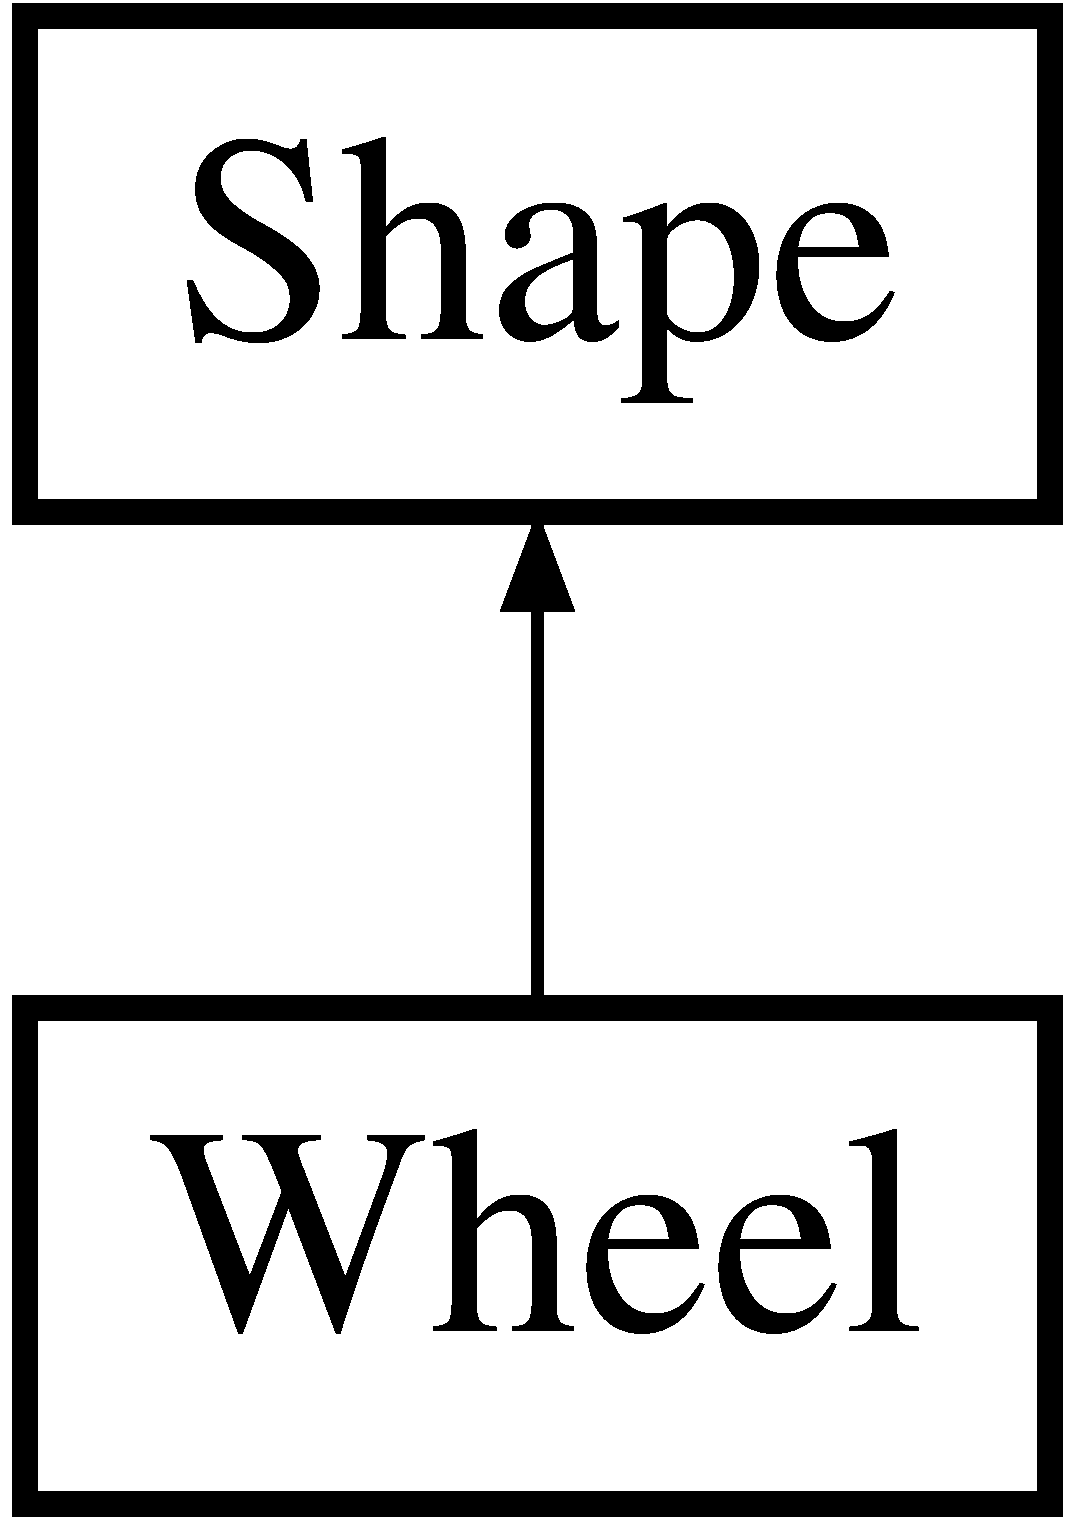
\includegraphics[height=2.000000cm]{classWheel}
\end{center}
\end{figure}
\subsection*{Public Member Functions}
\begin{DoxyCompactItemize}
\item 
\hyperlink{classWheel_a04a73ee48ea5d68a595aefdae58c2c03}{Wheel} (double x, double y, double w, double l, double sp, double ori, \hyperlink{Shape_8h_a5a4538eeab397888d88a4eefcc5a1345}{Shape\-Type} st, float c\mbox{[}3\mbox{]}, \hyperlink{Sensor_8h_a231524b302f9d7e6dd216fa89296f844}{Wheel\-I\-D} id)
\begin{DoxyCompactList}\small\item\em A Constructor. \end{DoxyCompactList}\end{DoxyCompactItemize}
\subsection*{Private Attributes}
\begin{DoxyCompactItemize}
\item 
\hyperlink{Sensor_8h_a231524b302f9d7e6dd216fa89296f844}{Wheel\-I\-D} \hyperlink{classWheel_aea86817285acade58673eaa82782ce7a}{I\-D}
\end{DoxyCompactItemize}


\subsection{Constructor \& Destructor Documentation}
\hypertarget{classWheel_a04a73ee48ea5d68a595aefdae58c2c03}{\index{Wheel@{Wheel}!Wheel@{Wheel}}
\index{Wheel@{Wheel}!Wheel@{Wheel}}
\subsubsection[{Wheel}]{\setlength{\rightskip}{0pt plus 5cm}Wheel\-::\-Wheel (
\begin{DoxyParamCaption}
\item[{double}]{x, }
\item[{double}]{y, }
\item[{double}]{w, }
\item[{double}]{l, }
\item[{double}]{sp, }
\item[{double}]{ori, }
\item[{{\bf Shape\-Type}}]{st, }
\item[{float}]{c\mbox{[}3\mbox{]}, }
\item[{{\bf Wheel\-I\-D}}]{id}
\end{DoxyParamCaption}
)}}\label{classWheel_a04a73ee48ea5d68a595aefdae58c2c03}


A Constructor. 

\begin{DoxyAuthor}{Author}
Zixiao Wang 
\end{DoxyAuthor}

\begin{DoxyParams}{Parameters}
{\em x} & The x position of \hyperlink{classShape}{Shape}. \\
\hline
{\em y} & The y position of \hyperlink{classShape}{Shape}. \\
\hline
{\em w} & The width of \hyperlink{classShape}{Shape}. \\
\hline
{\em l} & The length of \hyperlink{classShape}{Shape}. \\
\hline
{\em sp} & The speed of \hyperlink{classShape}{Shape}. \\
\hline
{\em ori} & The orientation of \hyperlink{classShape}{Shape}. \\
\hline
{\em st} & The Shape\-Type of \hyperlink{classShape}{Shape}. \\
\hline
{\em c} & The color of \hyperlink{classShape}{Shape}. \\
\hline
{\em id} & The I\-D of the wheel. \\
\hline
\end{DoxyParams}


\subsection{Member Data Documentation}
\hypertarget{classWheel_aea86817285acade58673eaa82782ce7a}{\index{Wheel@{Wheel}!I\-D@{I\-D}}
\index{I\-D@{I\-D}!Wheel@{Wheel}}
\subsubsection[{I\-D}]{\setlength{\rightskip}{0pt plus 5cm}{\bf Wheel\-I\-D} Wheel\-::\-I\-D\hspace{0.3cm}{\ttfamily [private]}}}\label{classWheel_aea86817285acade58673eaa82782ce7a}


The documentation for this class was generated from the following files\-:\begin{DoxyCompactItemize}
\item 
\hyperlink{Wheel_8h}{Wheel.\-h}\item 
\hyperlink{Wheel_8cpp}{Wheel.\-cpp}\end{DoxyCompactItemize}

\chapter{File Documentation}
\hypertarget{BaseGfxApp_8cpp}{\section{Base\-Gfx\-App.\-cpp File Reference}
\label{BaseGfxApp_8cpp}\index{Base\-Gfx\-App.\-cpp@{Base\-Gfx\-App.\-cpp}}
}
{\ttfamily \#include \char`\"{}Base\-Gfx\-App.\-h\char`\"{}}\\*
\subsection*{Macros}
\begin{DoxyCompactItemize}
\item 
\#define \hyperlink{BaseGfxApp_8cpp_a38533d3b08eadb4b2e6fe2f443dd83f1}{I\-N\-I\-T\-\_\-\-W\-I\-D\-T\-H}~800
\item 
\#define \hyperlink{BaseGfxApp_8cpp_acd7e35d0c6cca5b5b665b77b5377c4a0}{I\-N\-I\-T\-\_\-\-H\-E\-I\-G\-H\-T}~600
\end{DoxyCompactItemize}


\subsection{Macro Definition Documentation}
\hypertarget{BaseGfxApp_8cpp_acd7e35d0c6cca5b5b665b77b5377c4a0}{\index{Base\-Gfx\-App.\-cpp@{Base\-Gfx\-App.\-cpp}!I\-N\-I\-T\-\_\-\-H\-E\-I\-G\-H\-T@{I\-N\-I\-T\-\_\-\-H\-E\-I\-G\-H\-T}}
\index{I\-N\-I\-T\-\_\-\-H\-E\-I\-G\-H\-T@{I\-N\-I\-T\-\_\-\-H\-E\-I\-G\-H\-T}!BaseGfxApp.cpp@{Base\-Gfx\-App.\-cpp}}
\subsubsection[{I\-N\-I\-T\-\_\-\-H\-E\-I\-G\-H\-T}]{\setlength{\rightskip}{0pt plus 5cm}\#define I\-N\-I\-T\-\_\-\-H\-E\-I\-G\-H\-T~600}}\label{BaseGfxApp_8cpp_acd7e35d0c6cca5b5b665b77b5377c4a0}
\hypertarget{BaseGfxApp_8cpp_a38533d3b08eadb4b2e6fe2f443dd83f1}{\index{Base\-Gfx\-App.\-cpp@{Base\-Gfx\-App.\-cpp}!I\-N\-I\-T\-\_\-\-W\-I\-D\-T\-H@{I\-N\-I\-T\-\_\-\-W\-I\-D\-T\-H}}
\index{I\-N\-I\-T\-\_\-\-W\-I\-D\-T\-H@{I\-N\-I\-T\-\_\-\-W\-I\-D\-T\-H}!BaseGfxApp.cpp@{Base\-Gfx\-App.\-cpp}}
\subsubsection[{I\-N\-I\-T\-\_\-\-W\-I\-D\-T\-H}]{\setlength{\rightskip}{0pt plus 5cm}\#define I\-N\-I\-T\-\_\-\-W\-I\-D\-T\-H~800}}\label{BaseGfxApp_8cpp_a38533d3b08eadb4b2e6fe2f443dd83f1}

\hypertarget{BaseGfxApp_8h}{\section{Base\-Gfx\-App.\-h File Reference}
\label{BaseGfxApp_8h}\index{Base\-Gfx\-App.\-h@{Base\-Gfx\-App.\-h}}
}


The basic application class for C\-Sci-\/3081 project. Uses G\-L\-U\-T and G\-L\-U\-I and wraps them in a nice C++ interface.  


{\ttfamily \#include $<$string$>$}\\*
{\ttfamily \#include $<$iostream$>$}\\*
{\ttfamily \#include $<$assert.\-h$>$}\\*
{\ttfamily \#include $<$G\-L/glui.\-h$>$}\\*
\subsection*{Classes}
\begin{DoxyCompactItemize}
\item 
class \hyperlink{classBaseGfxApp}{Base\-Gfx\-App}
\end{DoxyCompactItemize}


\subsection{Detailed Description}
The basic application class for C\-Sci-\/3081 project. Uses G\-L\-U\-T and G\-L\-U\-I and wraps them in a nice C++ interface. \begin{DoxyAuthor}{Author}
C\-Sci3081 Guru 
\end{DoxyAuthor}

\hypertarget{EnvironmentClass_8cpp}{\section{Environment\-Class.\-cpp File Reference}
\label{EnvironmentClass_8cpp}\index{Environment\-Class.\-cpp@{Environment\-Class.\-cpp}}
}
{\ttfamily \#include \char`\"{}Environment\-Class.\-h\char`\"{}}\\*
{\ttfamily \#include $<$math.\-h$>$}\\*
{\ttfamily \#include $<$G\-L/glut.\-h$>$}\\*
{\ttfamily \#include $<$stdlib.\-h$>$}\\*

\hypertarget{EnvironmentClass_8h}{\section{Environment\-Class.\-h File Reference}
\label{EnvironmentClass_8h}\index{Environment\-Class.\-h@{Environment\-Class.\-h}}
}


Main application class for the Environment Class.  


{\ttfamily \#include \char`\"{}Robot\-Class.\-h\char`\"{}}\\*
{\ttfamily \#include \char`\"{}Light.\-h\char`\"{}}\\*
{\ttfamily \#include $<$vector$>$}\\*
{\ttfamily \#include $<$iostream$>$}\\*
\subsection*{Classes}
\begin{DoxyCompactItemize}
\item 
class \hyperlink{classEnvironmentClass}{Environment\-Class}
\end{DoxyCompactItemize}


\subsection{Detailed Description}
Main application class for the Environment Class. \begin{DoxyAuthor}{Author}
Group Meryl\-\_\-\-Streep 
\end{DoxyAuthor}
\begin{DoxyDate}{Date}
10 April 2015 
\end{DoxyDate}

\hypertarget{Light_8cpp}{\section{Light.\-cpp File Reference}
\label{Light_8cpp}\index{Light.\-cpp@{Light.\-cpp}}
}


The details of light.  


{\ttfamily \#include \char`\"{}Light.\-h\char`\"{}}\\*
{\ttfamily \#include $<$iostream$>$}\\*


\subsection{Detailed Description}
The details of light. \begin{DoxyAuthor}{Author}
Group Meryl\-\_\-\-Streep 
\end{DoxyAuthor}
\begin{DoxyDate}{Date}
10 April 2015 
\end{DoxyDate}

\hypertarget{Light_8h}{\section{Light.\-h File Reference}
\label{Light_8h}\index{Light.\-h@{Light.\-h}}
}


The representation of light within the simulation.  


{\ttfamily \#include $<$cstdlib$>$}\\*
{\ttfamily \#include \char`\"{}Shape.\-h\char`\"{}}\\*
\subsection*{Classes}
\begin{DoxyCompactItemize}
\item 
class \hyperlink{classLight}{Light}
\begin{DoxyCompactList}\small\item\em A light class contains attributes and behaviors. \end{DoxyCompactList}\end{DoxyCompactItemize}


\subsection{Detailed Description}
The representation of light within the simulation. \begin{DoxyAuthor}{Author}
Group Meryl\-\_\-\-Streep 
\end{DoxyAuthor}
\begin{DoxyDate}{Date}
8 April 2015 
\end{DoxyDate}

\hypertarget{main_8cpp}{\section{main.\-cpp File Reference}
\label{main_8cpp}\index{main.\-cpp@{main.\-cpp}}
}


Main function.  


{\ttfamily \#include \char`\"{}Simulation.\-h\char`\"{}}\\*
\subsection*{Functions}
\begin{DoxyCompactItemize}
\item 
int \hyperlink{main_8cpp_a0ddf1224851353fc92bfbff6f499fa97}{main} (int argc, char $\ast$argv\mbox{[}$\,$\mbox{]})
\end{DoxyCompactItemize}


\subsection{Detailed Description}
Main function. \begin{DoxyAuthor}{Author}
C\-Sci5107 Guru 
\end{DoxyAuthor}


\subsection{Function Documentation}
\hypertarget{main_8cpp_a0ddf1224851353fc92bfbff6f499fa97}{\index{main.\-cpp@{main.\-cpp}!main@{main}}
\index{main@{main}!main.cpp@{main.\-cpp}}
\subsubsection[{main}]{\setlength{\rightskip}{0pt plus 5cm}int main (
\begin{DoxyParamCaption}
\item[{int}]{argc, }
\item[{char $\ast$}]{argv\mbox{[}$\,$\mbox{]}}
\end{DoxyParamCaption}
)}}\label{main_8cpp_a0ddf1224851353fc92bfbff6f499fa97}

\hypertarget{RobotClass_8cpp}{\section{Robot\-Class.\-cpp File Reference}
\label{RobotClass_8cpp}\index{Robot\-Class.\-cpp@{Robot\-Class.\-cpp}}
}


The details of robot within the simulation.  


{\ttfamily \#include \char`\"{}Robot\-Class.\-h\char`\"{}}\\*
{\ttfamily \#include $<$iostream$>$}\\*
{\ttfamily \#include $<$stdlib.\-h$>$}\\*
{\ttfamily \#include $<$math.\-h$>$}\\*


\subsection{Detailed Description}
The details of robot within the simulation. \begin{DoxyAuthor}{Author}
Group Meryl\-\_\-\-Streep 
\end{DoxyAuthor}
\begin{DoxyDate}{Date}
10 April 2015 
\end{DoxyDate}

\hypertarget{RobotClass_8h}{\section{Robot\-Class.\-h File Reference}
\label{RobotClass_8h}\index{Robot\-Class.\-h@{Robot\-Class.\-h}}
}


The representation of robot within the simulation.  


{\ttfamily \#include $<$cstdlib$>$}\\*
{\ttfamily \#include \char`\"{}Shape.\-h\char`\"{}}\\*
{\ttfamily \#include \char`\"{}Wheel.\-h\char`\"{}}\\*
{\ttfamily \#include \char`\"{}Sensor.\-h\char`\"{}}\\*
{\ttfamily \#include $<$vector$>$}\\*
{\ttfamily \#include \char`\"{}Light.\-h\char`\"{}}\\*
\subsection*{Classes}
\begin{DoxyCompactItemize}
\item 
class \hyperlink{classRobotClass}{Robot\-Class}
\begin{DoxyCompactList}\small\item\em A robot class contains attributes and hehaviors. \end{DoxyCompactList}\end{DoxyCompactItemize}


\subsection{Detailed Description}
The representation of robot within the simulation. \begin{DoxyAuthor}{Author}
Group Meryl\-\_\-\-Streep 
\end{DoxyAuthor}
\begin{DoxyDate}{Date}
10 April 2015 
\end{DoxyDate}

\hypertarget{Sensor_8cpp}{\section{Sensor.\-cpp File Reference}
\label{Sensor_8cpp}\index{Sensor.\-cpp@{Sensor.\-cpp}}
}


The details of \hyperlink{classSensor}{Sensor}.  


{\ttfamily \#include \char`\"{}Sensor.\-h\char`\"{}}\\*
{\ttfamily \#include $<$iostream$>$}\\*
{\ttfamily \#include $<$math.\-h$>$}\\*
{\ttfamily \#include \char`\"{}Robot\-Class.\-h\char`\"{}}\\*


\subsection{Detailed Description}
The details of \hyperlink{classSensor}{Sensor}. \begin{DoxyAuthor}{Author}
Group Meryl\-\_\-\-Streep 
\end{DoxyAuthor}
\begin{DoxyDate}{Date}
10 April 2015 
\end{DoxyDate}

\hypertarget{Sensor_8h}{\section{Sensor.\-h File Reference}
\label{Sensor_8h}\index{Sensor.\-h@{Sensor.\-h}}
}


The representation of robot within the simulation.  


{\ttfamily \#include $<$cstdlib$>$}\\*
{\ttfamily \#include \char`\"{}Shape.\-h\char`\"{}}\\*
{\ttfamily \#include \char`\"{}Light.\-h\char`\"{}}\\*
{\ttfamily \#include $<$vector$>$}\\*
\subsection*{Classes}
\begin{DoxyCompactItemize}
\item 
class \hyperlink{classSensor}{Sensor}
\end{DoxyCompactItemize}
\subsection*{Enumerations}
\begin{DoxyCompactItemize}
\item 
enum \hyperlink{Sensor_8h_a213c434cb928c4ca22513e2302632435}{Sensor\-Type} \{ \hyperlink{Sensor_8h_a213c434cb928c4ca22513e2302632435a997f3ebaad078224014cca7ce7095537}{Robot\-Sensor}, 
\hyperlink{Sensor_8h_a213c434cb928c4ca22513e2302632435ad14f18d4e1c565acaa166edece9ba565}{Light\-Sensor}
 \}
\begin{DoxyCompactList}\small\item\em A light class contains attributes and hehaviors. \end{DoxyCompactList}\item 
enum \hyperlink{Sensor_8h_aa1f0e2efd52935fd01bfece0fbead81f}{Connection\-Type} \{ \hyperlink{Sensor_8h_aa1f0e2efd52935fd01bfece0fbead81faed960d16f6209c38ce7e3e79641468df}{Excitatorydirect}, 
\hyperlink{Sensor_8h_aa1f0e2efd52935fd01bfece0fbead81fab0f5c078185d0cb83bafdda1c186d0fb}{Excitatorycrossed}, 
\hyperlink{Sensor_8h_aa1f0e2efd52935fd01bfece0fbead81fabdd56a637ce0f5a8e28d5189ee6d0043}{Inhibitorydirect}, 
\hyperlink{Sensor_8h_aa1f0e2efd52935fd01bfece0fbead81fa82a969f36cd506e97ea21d658356c35b}{Inhibitorycrossed}
 \}
\begin{DoxyCompactList}\small\item\em connection types between sensor and wheel \end{DoxyCompactList}\item 
enum \hyperlink{Sensor_8h_a231524b302f9d7e6dd216fa89296f844}{Wheel\-I\-D} \{ \hyperlink{Sensor_8h_a231524b302f9d7e6dd216fa89296f844a0b7f0f6294e147e2e36d260241d4047b}{Left\-Wheel}, 
\hyperlink{Sensor_8h_a231524b302f9d7e6dd216fa89296f844a589ff6d02ae59889bc0d1ed9fbb91ebe}{Right\-Wheel}
 \}
\begin{DoxyCompactList}\small\item\em id for left and right wheel. \end{DoxyCompactList}\end{DoxyCompactItemize}


\subsection{Detailed Description}
The representation of robot within the simulation. \begin{DoxyAuthor}{Author}
Group Meryl\-\_\-\-Streep 
\end{DoxyAuthor}
\begin{DoxyDate}{Date}
15 Mar 2015 
\end{DoxyDate}


\subsection{Enumeration Type Documentation}
\hypertarget{Sensor_8h_aa1f0e2efd52935fd01bfece0fbead81f}{\index{Sensor.\-h@{Sensor.\-h}!Connection\-Type@{Connection\-Type}}
\index{Connection\-Type@{Connection\-Type}!Sensor.h@{Sensor.\-h}}
\subsubsection[{Connection\-Type}]{\setlength{\rightskip}{0pt plus 5cm}enum {\bf Connection\-Type}}}\label{Sensor_8h_aa1f0e2efd52935fd01bfece0fbead81f}


connection types between sensor and wheel 

\begin{Desc}
\item[Enumerator]\par
\begin{description}
\index{Excitatorydirect@{Excitatorydirect}!Sensor.\-h@{Sensor.\-h}}\index{Sensor.\-h@{Sensor.\-h}!Excitatorydirect@{Excitatorydirect}}\item[{\em 
\hypertarget{Sensor_8h_aa1f0e2efd52935fd01bfece0fbead81faed960d16f6209c38ce7e3e79641468df}{Excitatorydirect}\label{Sensor_8h_aa1f0e2efd52935fd01bfece0fbead81faed960d16f6209c38ce7e3e79641468df}
}]\index{Excitatorycrossed@{Excitatorycrossed}!Sensor.\-h@{Sensor.\-h}}\index{Sensor.\-h@{Sensor.\-h}!Excitatorycrossed@{Excitatorycrossed}}\item[{\em 
\hypertarget{Sensor_8h_aa1f0e2efd52935fd01bfece0fbead81fab0f5c078185d0cb83bafdda1c186d0fb}{Excitatorycrossed}\label{Sensor_8h_aa1f0e2efd52935fd01bfece0fbead81fab0f5c078185d0cb83bafdda1c186d0fb}
}]\index{Inhibitorydirect@{Inhibitorydirect}!Sensor.\-h@{Sensor.\-h}}\index{Sensor.\-h@{Sensor.\-h}!Inhibitorydirect@{Inhibitorydirect}}\item[{\em 
\hypertarget{Sensor_8h_aa1f0e2efd52935fd01bfece0fbead81fabdd56a637ce0f5a8e28d5189ee6d0043}{Inhibitorydirect}\label{Sensor_8h_aa1f0e2efd52935fd01bfece0fbead81fabdd56a637ce0f5a8e28d5189ee6d0043}
}]\index{Inhibitorycrossed@{Inhibitorycrossed}!Sensor.\-h@{Sensor.\-h}}\index{Sensor.\-h@{Sensor.\-h}!Inhibitorycrossed@{Inhibitorycrossed}}\item[{\em 
\hypertarget{Sensor_8h_aa1f0e2efd52935fd01bfece0fbead81fa82a969f36cd506e97ea21d658356c35b}{Inhibitorycrossed}\label{Sensor_8h_aa1f0e2efd52935fd01bfece0fbead81fa82a969f36cd506e97ea21d658356c35b}
}]\end{description}
\end{Desc}
\hypertarget{Sensor_8h_a213c434cb928c4ca22513e2302632435}{\index{Sensor.\-h@{Sensor.\-h}!Sensor\-Type@{Sensor\-Type}}
\index{Sensor\-Type@{Sensor\-Type}!Sensor.h@{Sensor.\-h}}
\subsubsection[{Sensor\-Type}]{\setlength{\rightskip}{0pt plus 5cm}enum {\bf Sensor\-Type}}}\label{Sensor_8h_a213c434cb928c4ca22513e2302632435}


A light class contains attributes and hehaviors. 

Inherit from \hyperlink{classShape}{Shape} class, add speed and orientation attributes. \hyperlink{classSensor}{Sensor} types for robots \begin{Desc}
\item[Enumerator]\par
\begin{description}
\index{Robot\-Sensor@{Robot\-Sensor}!Sensor.\-h@{Sensor.\-h}}\index{Sensor.\-h@{Sensor.\-h}!Robot\-Sensor@{Robot\-Sensor}}\item[{\em 
\hypertarget{Sensor_8h_a213c434cb928c4ca22513e2302632435a997f3ebaad078224014cca7ce7095537}{Robot\-Sensor}\label{Sensor_8h_a213c434cb928c4ca22513e2302632435a997f3ebaad078224014cca7ce7095537}
}]\index{Light\-Sensor@{Light\-Sensor}!Sensor.\-h@{Sensor.\-h}}\index{Sensor.\-h@{Sensor.\-h}!Light\-Sensor@{Light\-Sensor}}\item[{\em 
\hypertarget{Sensor_8h_a213c434cb928c4ca22513e2302632435ad14f18d4e1c565acaa166edece9ba565}{Light\-Sensor}\label{Sensor_8h_a213c434cb928c4ca22513e2302632435ad14f18d4e1c565acaa166edece9ba565}
}]\end{description}
\end{Desc}
\hypertarget{Sensor_8h_a231524b302f9d7e6dd216fa89296f844}{\index{Sensor.\-h@{Sensor.\-h}!Wheel\-I\-D@{Wheel\-I\-D}}
\index{Wheel\-I\-D@{Wheel\-I\-D}!Sensor.h@{Sensor.\-h}}
\subsubsection[{Wheel\-I\-D}]{\setlength{\rightskip}{0pt plus 5cm}enum {\bf Wheel\-I\-D}}}\label{Sensor_8h_a231524b302f9d7e6dd216fa89296f844}


id for left and right wheel. 

\begin{Desc}
\item[Enumerator]\par
\begin{description}
\index{Left\-Wheel@{Left\-Wheel}!Sensor.\-h@{Sensor.\-h}}\index{Sensor.\-h@{Sensor.\-h}!Left\-Wheel@{Left\-Wheel}}\item[{\em 
\hypertarget{Sensor_8h_a231524b302f9d7e6dd216fa89296f844a0b7f0f6294e147e2e36d260241d4047b}{Left\-Wheel}\label{Sensor_8h_a231524b302f9d7e6dd216fa89296f844a0b7f0f6294e147e2e36d260241d4047b}
}]\index{Right\-Wheel@{Right\-Wheel}!Sensor.\-h@{Sensor.\-h}}\index{Sensor.\-h@{Sensor.\-h}!Right\-Wheel@{Right\-Wheel}}\item[{\em 
\hypertarget{Sensor_8h_a231524b302f9d7e6dd216fa89296f844a589ff6d02ae59889bc0d1ed9fbb91ebe}{Right\-Wheel}\label{Sensor_8h_a231524b302f9d7e6dd216fa89296f844a589ff6d02ae59889bc0d1ed9fbb91ebe}
}]\end{description}
\end{Desc}

\hypertarget{Shape_8cpp}{\section{Shape.\-cpp File Reference}
\label{Shape_8cpp}\index{Shape.\-cpp@{Shape.\-cpp}}
}


Details of \hyperlink{classShape}{Shape(super class)}  


{\ttfamily \#include \char`\"{}Shape.\-h\char`\"{}}\\*
{\ttfamily \#include $<$iostream$>$}\\*


\subsection{Detailed Description}
Details of \hyperlink{classShape}{Shape(super class)} \begin{DoxyAuthor}{Author}
Group Meryl\-\_\-\-Streep 
\end{DoxyAuthor}
\begin{DoxyDate}{Date}
10 April 2015 
\end{DoxyDate}

\hypertarget{Shape_8h}{\section{Shape.\-h File Reference}
\label{Shape_8h}\index{Shape.\-h@{Shape.\-h}}
}


The Super Class.  


{\ttfamily \#include $<$cstdlib$>$}\\*
{\ttfamily \#include $<$time.\-h$>$}\\*
{\ttfamily \#include $<$math.\-h$>$}\\*
\subsection*{Classes}
\begin{DoxyCompactItemize}
\item 
class \hyperlink{classShape}{Shape}
\begin{DoxyCompactList}\small\item\em Super Class of \hyperlink{classRobotClass}{Robot\-Class}, Target and Obstacle, contains position x, y, width and length. \end{DoxyCompactList}\end{DoxyCompactItemize}
\subsection*{Enumerations}
\begin{DoxyCompactItemize}
\item 
enum \hyperlink{Shape_8h_a5a4538eeab397888d88a4eefcc5a1345}{Shape\-Type} \{ \hyperlink{Shape_8h_a5a4538eeab397888d88a4eefcc5a1345ad3ce82743a8255ccd69f5b67d257c489}{Circle}, 
\hyperlink{Shape_8h_a5a4538eeab397888d88a4eefcc5a1345a773e9be14af3bc697c412f3e6c5c509e}{Triangle}, 
\hyperlink{Shape_8h_a5a4538eeab397888d88a4eefcc5a1345ad614565f121617f9b952559339bffcf6}{Rectangle}, 
\hyperlink{Shape_8h_a5a4538eeab397888d88a4eefcc5a1345a349990a9494411f297f9349ed29172b3}{Quad}
 \}
\item 
enum \hyperlink{Shape_8h_ad4f6886266572e51d198a61a6c762ce5}{Wall} \{ \\*
\hyperlink{Shape_8h_ad4f6886266572e51d198a61a6c762ce5ac9d3e887722f2bc482bcca9d41c512af}{None}, 
\hyperlink{Shape_8h_ad4f6886266572e51d198a61a6c762ce5a47321105d20c4efd6c573a6d829e1ad9}{Top}, 
\hyperlink{Shape_8h_ad4f6886266572e51d198a61a6c762ce5a05cdd4fa6b505ee008f4e865acfecccb}{Bottom}, 
\hyperlink{Shape_8h_ad4f6886266572e51d198a61a6c762ce5a9d4d8b0b72fc2659da772d761a3c5ecb}{Left}, 
\\*
\hyperlink{Shape_8h_ad4f6886266572e51d198a61a6c762ce5ad48f7af8c070184f3774c8e85854eb66}{Right}
 \}
\end{DoxyCompactItemize}


\subsection{Detailed Description}
The Super Class. \begin{DoxyAuthor}{Author}
Group Meryl\-\_\-\-Streep 
\end{DoxyAuthor}
\begin{DoxyDate}{Date}
8 April 2015 
\end{DoxyDate}


\subsection{Enumeration Type Documentation}
\hypertarget{Shape_8h_a5a4538eeab397888d88a4eefcc5a1345}{\index{Shape.\-h@{Shape.\-h}!Shape\-Type@{Shape\-Type}}
\index{Shape\-Type@{Shape\-Type}!Shape.h@{Shape.\-h}}
\subsubsection[{Shape\-Type}]{\setlength{\rightskip}{0pt plus 5cm}enum {\bf Shape\-Type}}}\label{Shape_8h_a5a4538eeab397888d88a4eefcc5a1345}
\begin{Desc}
\item[Enumerator]\par
\begin{description}
\index{Circle@{Circle}!Shape.\-h@{Shape.\-h}}\index{Shape.\-h@{Shape.\-h}!Circle@{Circle}}\item[{\em 
\hypertarget{Shape_8h_a5a4538eeab397888d88a4eefcc5a1345ad3ce82743a8255ccd69f5b67d257c489}{Circle}\label{Shape_8h_a5a4538eeab397888d88a4eefcc5a1345ad3ce82743a8255ccd69f5b67d257c489}
}]\hyperlink{classShape}{Shape} type of Object \index{Triangle@{Triangle}!Shape.\-h@{Shape.\-h}}\index{Shape.\-h@{Shape.\-h}!Triangle@{Triangle}}\item[{\em 
\hypertarget{Shape_8h_a5a4538eeab397888d88a4eefcc5a1345a773e9be14af3bc697c412f3e6c5c509e}{Triangle}\label{Shape_8h_a5a4538eeab397888d88a4eefcc5a1345a773e9be14af3bc697c412f3e6c5c509e}
}]\index{Rectangle@{Rectangle}!Shape.\-h@{Shape.\-h}}\index{Shape.\-h@{Shape.\-h}!Rectangle@{Rectangle}}\item[{\em 
\hypertarget{Shape_8h_a5a4538eeab397888d88a4eefcc5a1345ad614565f121617f9b952559339bffcf6}{Rectangle}\label{Shape_8h_a5a4538eeab397888d88a4eefcc5a1345ad614565f121617f9b952559339bffcf6}
}]\index{Quad@{Quad}!Shape.\-h@{Shape.\-h}}\index{Shape.\-h@{Shape.\-h}!Quad@{Quad}}\item[{\em 
\hypertarget{Shape_8h_a5a4538eeab397888d88a4eefcc5a1345a349990a9494411f297f9349ed29172b3}{Quad}\label{Shape_8h_a5a4538eeab397888d88a4eefcc5a1345a349990a9494411f297f9349ed29172b3}
}]\end{description}
\end{Desc}
\hypertarget{Shape_8h_ad4f6886266572e51d198a61a6c762ce5}{\index{Shape.\-h@{Shape.\-h}!Wall@{Wall}}
\index{Wall@{Wall}!Shape.h@{Shape.\-h}}
\subsubsection[{Wall}]{\setlength{\rightskip}{0pt plus 5cm}enum {\bf Wall}}}\label{Shape_8h_ad4f6886266572e51d198a61a6c762ce5}
\begin{Desc}
\item[Enumerator]\par
\begin{description}
\index{None@{None}!Shape.\-h@{Shape.\-h}}\index{Shape.\-h@{Shape.\-h}!None@{None}}\item[{\em 
\hypertarget{Shape_8h_ad4f6886266572e51d198a61a6c762ce5ac9d3e887722f2bc482bcca9d41c512af}{None}\label{Shape_8h_ad4f6886266572e51d198a61a6c762ce5ac9d3e887722f2bc482bcca9d41c512af}
}]Different walls \index{Top@{Top}!Shape.\-h@{Shape.\-h}}\index{Shape.\-h@{Shape.\-h}!Top@{Top}}\item[{\em 
\hypertarget{Shape_8h_ad4f6886266572e51d198a61a6c762ce5a47321105d20c4efd6c573a6d829e1ad9}{Top}\label{Shape_8h_ad4f6886266572e51d198a61a6c762ce5a47321105d20c4efd6c573a6d829e1ad9}
}]\index{Bottom@{Bottom}!Shape.\-h@{Shape.\-h}}\index{Shape.\-h@{Shape.\-h}!Bottom@{Bottom}}\item[{\em 
\hypertarget{Shape_8h_ad4f6886266572e51d198a61a6c762ce5a05cdd4fa6b505ee008f4e865acfecccb}{Bottom}\label{Shape_8h_ad4f6886266572e51d198a61a6c762ce5a05cdd4fa6b505ee008f4e865acfecccb}
}]\index{Left@{Left}!Shape.\-h@{Shape.\-h}}\index{Shape.\-h@{Shape.\-h}!Left@{Left}}\item[{\em 
\hypertarget{Shape_8h_ad4f6886266572e51d198a61a6c762ce5a9d4d8b0b72fc2659da772d761a3c5ecb}{Left}\label{Shape_8h_ad4f6886266572e51d198a61a6c762ce5a9d4d8b0b72fc2659da772d761a3c5ecb}
}]\index{Right@{Right}!Shape.\-h@{Shape.\-h}}\index{Shape.\-h@{Shape.\-h}!Right@{Right}}\item[{\em 
\hypertarget{Shape_8h_ad4f6886266572e51d198a61a6c762ce5ad48f7af8c070184f3774c8e85854eb66}{Right}\label{Shape_8h_ad4f6886266572e51d198a61a6c762ce5ad48f7af8c070184f3774c8e85854eb66}
}]\end{description}
\end{Desc}

\hypertarget{Simulation_8cpp}{\section{Simulation.\-cpp File Reference}
\label{Simulation_8cpp}\index{Simulation.\-cpp@{Simulation.\-cpp}}
}
{\ttfamily \#include \char`\"{}Simulation.\-h\char`\"{}}\\*
{\ttfamily \#include $<$math.\-h$>$}\\*
{\ttfamily \#include $<$time.\-h$>$}\\*

\hypertarget{Simulation_8h}{\section{Simulation.\-h File Reference}
\label{Simulation_8h}\index{Simulation.\-h@{Simulation.\-h}}
}


Main application class for the robot simulation.  


{\ttfamily \#include $<$vector$>$}\\*
{\ttfamily \#include $<$cstdlib$>$}\\*
{\ttfamily \#include \char`\"{}Base\-Gfx\-App.\-h\char`\"{}}\\*
{\ttfamily \#include \char`\"{}Environment\-Class.\-h\char`\"{}}\\*
{\ttfamily \#include \char`\"{}Object.\-h\char`\"{}}\\*
\subsection*{Classes}
\begin{DoxyCompactItemize}
\item 
class \hyperlink{classSimulation}{Simulation}
\end{DoxyCompactItemize}


\subsection{Detailed Description}
Main application class for the robot simulation. \begin{DoxyAuthor}{Author}
C\-Sci3081 Guru 
\end{DoxyAuthor}

\hypertarget{Wheel_8cpp}{\section{Wheel.\-cpp File Reference}
\label{Wheel_8cpp}\index{Wheel.\-cpp@{Wheel.\-cpp}}
}
{\ttfamily \#include \char`\"{}Wheel.\-h\char`\"{}}\\*
{\ttfamily \#include $<$iostream$>$}\\*

\hypertarget{Wheel_8h}{\section{Wheel.\-h File Reference}
\label{Wheel_8h}\index{Wheel.\-h@{Wheel.\-h}}
}
{\ttfamily \#include $<$stdlib.\-h$>$}\\*
{\ttfamily \#include \char`\"{}Shape.\-h\char`\"{}}\\*
{\ttfamily \#include \char`\"{}Sensor.\-h\char`\"{}}\\*
\subsection*{Classes}
\begin{DoxyCompactItemize}
\item 
class \hyperlink{classWheel}{Wheel}
\end{DoxyCompactItemize}

%--- End generated contents ---

% Index
\newpage
\phantomsection
\addcontentsline{toc}{chapter}{Index}
\printindex

\end{document}
